% !Mode:: "TeX:UTF-8"
%# -*- coding:utf-8 -*-

%% 南京大学学位论文的示例文档
%% 作者:njuhan: https://github.com/njuHan
%% 源模版repo: https://github.com/njuHan/njuthesis-nju-thesis-template

\documentclass[winfonts,master,twoside]{njuthesis}
%% njuthesis 文档类的可选参数有:
%%   winfonts, linuxfonts, macfonts, adobefonts winfonts 选项使得文档使用Windows 系统提供的字体;linuxfonts 选项使得文档使用Linux 系统提供的字体;macfonts 选项使得文档使用Mac 系统提供的字体;adobefonts 选项使得文档使用Adobe提供的OTF中文字体(需自行下载安转)
%%   phd/master/bachelor 选择博士/硕士/学士论文
%%   twoside 或 oneside 指定排版的文档为双面打印或单面打印格式(twoside会使得chapter 章节从奇数页开始,即纸张的正面开始,因此会出现一些空白的页面)
%%   nobackinfo 取消封二页导师签名信息。注意,按照南大的规定,是需要签名页的。

\lstset{
	columns=fixed,       
	basicstyle=\small,
	numbers=left,                                        % 在左侧显示行号
	numberstyle=\tiny\color{gray},                       % 设定行号格式
	frame=none,                                          % 不显示背景边框
	backgroundcolor=\color[RGB]{245,245,244},            % 设定背景颜色
	keywordstyle=\color[RGB]{40,40,255},                 % 设定关键字颜色
	numberstyle=\footnotesize\color{darkgray},           
	commentstyle=\it\color[RGB]{0,96,96},                % 设置代码注释的格式
	stringstyle=\rmfamily\slshape\color[RGB]{128,0,0},   % 设置字符串格式
	showstringspaces=false,                              % 不显示字符串中的空格
}
\renewcommand{\lstlistingname}{代码}

%%%%%%%%%%%%%%%%%%%%%%%%%%%%%%%%%%%%%%%%%%%%%%%%%%%%%%%%%%%%%%%%%%%%%%%%%%%%%%%
% set up labelformat and labelsep for subfigure 详见: http://www.latexstudio.net/archives/8652.html
\captionsetup[subfigure]{labelformat=simple, labelsep=space}

%%%%%%%%%%%%%%%%%%%%%%%%%%%%%%%%%%%%%%%%%%%%%%%%%%%%%%%%%%%%%%%%%%%%%%%%%%%%%%%
% 设置论文的中文封面

% 单行论文标题,不可换行
\title{定制Android系统服务测试技术研究}

% 如果论文标题过长,可以分两行,第一行用\titlea{}定义,第二行用\titleb{}定义,
% 使用以下3行:
%\title{} %用于覆盖单行标题内容为空
%\titlea{长标题第一行}  %第一行标题写这里
%\titleb{长标题第二行用于长标题换行} %第二行标题写这里
% 注意: \title 不能都注释,它用于控制标题选择双行还是单行。\title{}如果内容为空,则编译\titlea{},titleb{}双行标题,否则编译单行标题


% 论文作者姓名
\author{廖祥森}
% 论文作者联系电话
\telphone{-}
% 论文作者电子邮件地址
\email{-}
% 论文作者学生证号
\studentnum{-}
% 论文作者入学年份(年级)
\grade{2018}
% 论文作者毕业年份(届), 出版授权书的学位年度
\graduateyear{2021}
% 导师姓名职称
\supervisor{曹春~~教授}
% 导师的联系电话
\supervisortelphone{}
% 论文作者的学科与专业方向
\major{计算机技术}
% 论文作者的研究方向
\researchfield{软件方法学}
% 论文作者所在院系的中文名称
\department{计算机科学与技术系}
% 论文作者所在学校或机构的名称。此属性可选,默认值为``南京大学''。
\institute{南京大学}
% 论文的提交日期,需设置年、月、日。
\submitdate{2021年 05 月 29 日}
% 论文的答辩日期,需设置年、月、日。
\defenddate{2021年 05 月 25 日}
% 论文的定稿日期,需设置年、月、日。
% 此属性可选,若注释\date{},则默认值为最后一次编译时的日期,精确到日。
\date{2021年 05 月 29 日}

%%%%%%%%%%%%%%%%%%%%%%%%%%%%%%%%%%%%%%%%%%%%%%%%%%%%%%%%%%%%%%%%%%%%%%%%%%%%%%%
% 设置论文的英文封面

% 论文的英文标题,不可换行
\englishtitle{Research of Service Testing in Vendor Android}
% 论文作者姓名的拼音
\englishauthor{LIAO Xiangsen}
% 导师姓名职称的英文
\englishsupervisor{Professor CAO Chun}
% 论文作者学科与专业的英文名
\englishmajor{Computer Technology}
% 论文作者所在院系的英文名称
\englishdepartment{Department of Computer Science and Technology}
% 论文作者所在学校或机构的英文名称。此属性可选,默认值为``Nanjing University''。
\englishinstitute{Nanjing University}
% 论文完成日期的英文形式,它将出现在英文封面下方。需设置年、月、日。日期格式使用美国的日期
% 格式,即``Month day, year'',其中``Month''为月份的英文名全称,首字母大写;``day''为
% 该月中日期的阿拉伯数字表示;``year''为年份的四位阿拉伯数字表示。
% 此属性可选,若注释掉\englishdate{},则默认值为最后一次编译时的日期。
\englishdate{May 29, 2021}

%%%%%%%%%%%%%%%%%%%%%%%%%%%%%%%%%%%%%%%%%%%%%%%%%%%%%%%%%%%%%%%%%%%%%%%%%%%%%%%
% 设置论文的中文摘要

% 设置中文摘要页面的论文标题及副标题的第一行。
% 此属性可选,其默认值为使用|\title|命令所设置的论文标题
\abstracttitlea{定制Android系统服务测试技术研究}
% 设置中文摘要页面的论文标题及副标题的第二行。
% 此属性可选,其默认值为空白
%\abstracttitleb{定制Android系统服务测试技术研究}

%%%%%%%%%%%%%%%%%%%%%%%%%%%%%%%%%%%%%%%%%%%%%%%%%%%%%%%%%%%%%%%%%%%%%%%%%%%%%%%
% 设置论文的英文摘要

% 设置英文摘要页面的论文标题及副标题的第一行。
% 此属性可选,其默认值为使用|\englishtitle|命令所设置的论文标题
\englishabstracttitlea{Research of Service Testing in Vendor Android}
% 设置英文摘要页面的论文标题及副标题的第二行。
% 此属性可选,其默认值为空白
%\englishabstracttitleb{nglishabstracttitleb}

%%%%%%%%%%%%%%%%%%%%%%%%%%%%%%%%%%%%%%%%%%%%%%%%%%%%%%%%%%%%%%%%%%%%%%%%%%%%%%
%% 盲审命令,空白字段设置请看 .cls文件 \newcommand*{\blind}
%% 此外,请按照盲审要求自行去掉个人简历、致谢等页面中的个人信息
%\blind

%%%%%%%%%%%%%%%%%%%%%%%%%%%%%%%%%%%%%%%%%%%%%%%%%%%%%%%%%%%%%%%%%%%%%%%%%%%%%%%
\begin{document}

%%%%%%%%%%%%%%%%%%%%%%%%%%%%%%%%%%%%%%%%%%%%%%%%%%%%%%%%%%%%%%%%%%%%%%%%%%%%%%%

% 制作国家图书馆封面(博士学位论文才需要)
%\makenlctitle
% 制作中文封面
\maketitle
% 制作英文封面
\makeenglishtitle


%%%%%%%%%%%%%%%%%%%%%%%%%%%%%%%%%%%%%%%%%%%%%%%%%%%%%%%%%%%%%%%%%%%%%%%%%%%%%%%
% 开始前言部分
\frontmatter

%%%%%%%%%%%%%%%%%%%%%%%%%%%%%%%%%%%%%%%%%%%%%%%%%%%%%%%%%%%%%%%%%%%%%%%%%%%%%%%
% 论文的中文摘要
\begin{abstract}

当前Android系统已成为最主要的移动互联网平台,并且Android的技术开放性为移动设备厂商对官方系统进行定制化开发提供了便利。相关研究表明,这些定制化的Android系统,特别是其引入的大量服务扩大了Android系统的攻击面。为了保障定制Android系统的安全性,研究并实现对其中服务的有效测试成为必要。针对现有服务模糊测试工作中因缺乏服务接口签名导致的测试效率低下问题,提出一种服务接口签名逆向提取方法,以指导测试用例的生成。在服务模糊测试过程中,通过模拟Android系统上下文提高测试深度,生成异常IBinder类型更有效地测试服务的边界情况。

具体而言,本文的工作主要包括:

\begin{itemize}
	\item 提出一种使用逆向工程自动化提取服务接口签名的方法,可从Java与Native服务的编译产物中,通过对Binder通信序列化函数结构的还原,逆向推测出服务接口签名,并实现了服务接口签名提取工具RevExtractor。
	\item 实现了一个服务模糊测试工具CASFuzzer:基于服务接口签名指导测试用例的生成与变异;通过Binder通信劫持技术,模拟影响服务执行的Android系统上下文,提高测试深度;动态地构造通用服务对象,以模拟Android系统中特有的IBinder类型的异常行为,更好地测试服务的边界情况。
	\item 在两个主流的定制Android系统上进行实验评估。实验结果表明,服务接口签名提取工具RevExtractor具有较高的准确性,服务模糊测试工具CASFuzzer中对Android系统上下文的模拟使得测试过程更加深入有效,测试用例中构造的异常IBinder类型可以触发特定的服务缺陷。
\end{itemize}

% 中文关键词。关键词之间用中文全角分号隔开,末尾无标点符号。
\keywords{Android;模糊测试;逆向工程;Binder}
\end{abstract}

%%%%%%%%%%%%%%%%%%%%%%%%%%%%%%%%%%%%%%%%%%%%%%%%%%%%%%%%%%%%%%%%%%%%%%%%%%%%%%%
% 论文的英文摘要
\begin{englishabstract}

Android is the most popular operating system of smartphone. It's convenient to customize the Android for mobile device manufacturers. Related research shows that the Vendor Android, which adds a large number of Services, has expanded the attack surface of Android. In order to ensure the security of the Vendor Android, it is necessary to test its Services effectively. Most related works are mutation-based fuzzers, they have low code coverage of target Services due to the lack of type signature. So we design a reverse engineering method to extracte Service signature in closed-source Vendor Android. We implement a generation-based Service fuzzing tool, to improve the test depth through mocked Android Context, and to test the Service boundary conditions more effectively through abnormal IBinder type. The main work is as follow:
\begin{itemize}
	\item A reverse engineering method to extract the Service signature automatically. From the compiled artifacts of Java and Native Services, the Service signature can be reversely inferred by restoring the structure in the Binder serialization function.
	\item We implement a Service fuzzing tool, CASFuzzer: it can generate and mutate test case based on the Service signature; through Binder IPC interception technology, it can mock Android Context that affects the execution of the service to improve the depth of testing; through dynamic general ServiceStub, it can generate abnormal IBinder type for boundary condition testing of the Service.
	\item We evalute our tools with two popular Vendor Android OS. The experimental results show that the Service signature extraction tool RevExtractor has high accuracy. The simulation of the Android Context makes the testing more in-depth and effective. The abnormal IBinder type can trigger specific Service defects.
\end{itemize}

% 英文关键词。关键词之间用英文半角逗号隔开,末尾无符号。
\englishkeywords{Android, Fuzzing, Reverse Engineering, Binder}

\end{englishabstract}

%%%%%%%%%%%%%%%%%%%%%%%%%%%%%%%%%%%%%%%%%%%%%%%%%%%%%%%%%%%%%%%%%%%%%%%%%%%%%%%
% 生成论文目录
\tableofcontents

%%%%%%%%%%%%%%%%%%%%%%%%%%%%%%%%%%%%%%%%%%%%%%%%%%%%%%%%%%%%%%%%%%%%%%%%%%%%%%%
% 生成插图清单。如无需插图清单则可注释掉下述语句。
\listoffigures

%%%%%%%%%%%%%%%%%%%%%%%%%%%%%%%%%%%%%%%%%%%%%%%%%%%%%%%%%%%%%%%%%%%%%%%%%%%%%%%
% 生成附表清单。如无需附表清单则可注释掉下述语句。
\listoftables

%%%%%%%%%%%%%%%%%%%%%%%%%%%%%%%%%%%%%%%%%%%%%%%%%%%%%%%%%%%%%%%%%%%%%%%%%%%%%%%
% 开始正文部分
\mainmatter

%%%%%%%%%%%%%%%%%%%%%%%%%%%%%%%%%%%%%%%%%%%%%%%%%%%%%%%%%%%%%%%%%%%%%%%%%%%%%%%
% 学位论文的正文应以《绪论》作为第一章
\chapter{绪论}\label{chapter_introduction}
\section{研究背景及意义}

作为移动互联网时代的主要终端设备,智能手机得到了广泛的应用,在当前智能手机市场份额中,Google公司开发的Android系统占据了主导地位(根据IDC对移动端操作系统的最新统计\cite{smartphoneos}显示,Android系统的市场占有率高达84.1\%)。除了智能手机以外,Android系统同样也在物联网终端,如智能电视、智能汽车等设备上得到了广泛应用。相较于其他操作系统,Android系统最大的优势在于它的开放性,Google公司允许任何设备厂商加入到Android开发联盟中来。

Android系统的开放性吸引了越来越多的终端应用开发者,Android生态圈在短时间内积累了丰富的软件资源和大量的用户。随着用户日常生活与手机越来越紧密相连,手机中存储着用户大量的个人隐私信息,这也吸引了越来越多攻击者的注意。当前Android生态圈的安全问题不容忽视:根据CVE Detail的统计\cite{CVE}显示,Android系统常年位居各类操作系统漏洞数量榜前列;2019年,360安全大脑共截获移动端新增恶意程序样本180.9万个,平均每天新截获5000个恶意程序样本\cite{360-mobile-security};腾讯安全发布的手机安全报告\cite{tencent-mobile-security}中指出,2020上半年手机病毒感染用户数3058.95万,新增Android病毒包308.05万个,同比涨幅达62.24\%;漏洞收购平台Zerodium更是给Android漏洞完整利用链开出了250万美元的“悬赏”,远超其他操作系统\cite{zerodium}。

移动设备厂商为了提高自家手机的产品竞争力,不仅会在硬件配置上体现出差异与特色,还会对Android系统本身进行二次开发以提供更丰富的功能。除此之外,为了使得手机用户可以开箱即用,厂商定制的Android系统中往往会预装自己的一套系统应用,比如应用商店、手机钱包、视频播放器、桌面美化软件等等。出于性能和用户体验考虑,还可能采取安全性弱化的软件配置。相关研究表明,相较于Google官方的Android系统,厂商对Android系统的定制化引入了更多的安全隐患\cite{gallo2015security}\cite{aafer2016harvesting}\cite{farhang2020empirical}。

Android生态圈的碎片化现象是导致其安全隐患的重要因素。具不完全统计,市面上有超过200家移动设备厂商提供的超过7000种Android智能设备\cite{android-brands},设备上搭载的定制Android系统也不尽相同。这使得上游的Google公司很难对这样一个开放、多样化的软件生态系统进行很好的质量管理。如何保证这些定制Android系统的安全性,发掘其中的安全漏洞具有重要的研究价值。

服务(Service)是Android系统的核心组成部分,服务除了以组件的形式广泛分布于Android应用之中,Android系统的绝大多数功能也是通过系统服务的形式暴露给上层使用,对于攻击者来说,服务是一个很好的攻击面。定制Android系统中不仅包含了大量的预装应用服务组件,而且引入了更多的系统服务(如Samsung Experience 8.0系统中添加了多达82个系统服务\cite{iannillo2017chizpurfle}),这些具有系统关键权限的服务进一步扩大了Android系统的攻击面。因此,对服务进行测试有助于保障定制Android系统的安全性,具有重要的研究价值。

\section{研究现状}\label{subsec:mptcp_conges}

软件漏洞挖掘技术自软件诞生之初一直是一个热门的研究领域。根据是否执行待测程序,漏洞挖掘技术可分为静态分析、动态分析与混合分析三类\cite{ji2018coming}。静态分析直接对程序源码进行检测,可以获得较高的代码覆盖率,并容易发现程序的边界情况,但会面临路径爆炸以及约束求解开销过大等问题;动态分析能获得程序的执行状态,但对代码分支路径的覆盖不够全面。

基于静态程序分析的符号执行(symbolic execution)与基于动态执行的模糊测试(fuzzing)是当前主流、也是最有效的漏洞挖掘技术。

符号执行技术最早由King等人提出\cite{king1976symbolic},目前KLEE \cite{cadar2008klee}是使用最为广泛的符号执行引擎。符号执行技术通过分析待测程序来得到程序特定执行路径的输入,其关键思路是维护一个程序执行路径的约束条件集合,以符号代替具体数值作为输入,遇到程序分支时将分支判断条件加入到约束条件集合中,最后将约束条件集合输入约束求解器,生成与此路径所对应的具体程序输入。

模糊测试技术最早由Millor等人提出,用于测试UNIX系统中的工具类程序\cite{miller1990empirical}。模糊测试技术是一种黑盒或灰盒的测试技术,通过自动化生成并输入大量的随机测试用例以检测待测程序中的漏洞。

在Android领域的相关研究中,Luo等人实现的CENTAUR \cite{luo2016context}首次将符号执行技术应用到Android系统服务的测试之上,并结合了具体执行(concrete execution)收集的Android系统上下文状态,以避免符号执行陷入系统服务初始化阶段。然而对于Android这样一个复杂并且组件化的系统来说,符号执行等静态程序分析技术会面临控制流图不完整、状态爆炸等问题。模糊测试技术由于其自动化程度高、可拓展性强被广泛应用于Android领域的服务漏洞挖掘之中。

模糊测试技术主要分为两类\cite{li2018fuzzing}:基于变异(mutation-based fuzzing),根据已有的测试用例样本,通过变异的方法生成新的测试用例;基于生成(generation-based fuzzing),根据待测程序的协议或接口规范进行建模,基于模型生成测试用例。已有对Android服务的测试工作大多使用了模糊测试技术,以下介绍五个代表性工作以及他们的局限性。

Zhang等人的研究\cite{zhang2017systematically}以Intent为服务通信接口,对Android应用中的Java后台服务进行测试。研究指出提高测试效率的关键是构造可成功启动服务的Intent对象。对待测服务的入口函数onStartCommand进行局部的静态分析,识别出Intent中action、component、category等字段的值,利用NLP方法推断出extras的value类型。然而只能用于启动式服务的测试,并不适用于以AIDL为通信接口\cite{service}的绑定式服务。

BinderCracker \cite{feng2016understanding}以Binder为服务通信接口,对Android中的系统服务进行黑盒测试。通过对通信过程的监控,记录下Binder驱动收到的消息体,对消息体进行变异以构造新的测试用例。纯粹基于变异的方法很难构造有效的测试用例,测试的效率不高。

Gu等人的研究\cite{gu2016exploiting}将关注点放在Android SDK中Service Helper(Service Helper封装了系统服务的功能,上层应用往往通过Service Helper间接与系统服务进行通信)与系统服务接口在权限检查上的不一致性,使用静态分析的方法比较这两者在实现逻辑上的差异,进而识别出Service Helper的安全隐患。

Chizpurfle \cite{iannillo2017chizpurfle}以AIDL为服务通信接口,对定制Android系统中的Java系统服务进行测试。通过Java反射获取待测服务的接口签名,以生成合法的输入参数;并结合二进制插桩技术统计待测服务的代码覆盖率,使用覆盖率指导的模糊测试技术(coverage-guided fuzzing)对服务进行测试。局限在于只考虑了Java类型的服务,事实上某些定制Android系统中有将近一半的系统服务以C++代码的形式实现。


FANS \cite{liu2020fans}以AIDL为服务通信接口,对AOSP中的Native系统服务进行测试。对通信部分的C++代码进行静态分析,以获取待测服务的接口签名,并尝试从变量类型、变量名称等属性推测不同接口的依赖关系,以此构造多层次的类型模型,指导测试用例的生成。局限在于必须获得待测服务的源码,不能适用于定制Android系统中的闭源服务。


\section{本文主要工作}

基于生成式策略的模糊测试方法由于对程序输入有更精确的类型模型,减少了不合法输入,在针对具有高度结构化特征的Android服务接口输入时,相较于基于变异策略的测试方法更为有效。

生成式策略的关键在于获取程序输入的类型模型,然而针对于定制Android系统中的Java以及Native服务来说,以往基于Java反射\cite{iannillo2017chizpurfle}、基于AIDL接口定义\cite{gu2016exploiting}、基于C++源码静态分析\cite{liu2020fans}等类型模型提取方法并不完全适用。本文提出一种服务接口签名自动化提取方法,从逆向工程的角度分析服务的编译产物,识别其中通信序列化过程的代码结构特征,以此推断出服务接口签名。接着基于生成式策略实现了一个服务模糊测试工具,输入服务接口签名以指导测试用例的生成与变异,通过Binder通信劫持技术以模拟其中的动态类型信息,测试迭代时通过动态二进制插桩技术收集基本块覆盖信息,以评估测试效果。

\begin{figure}
	\centering
	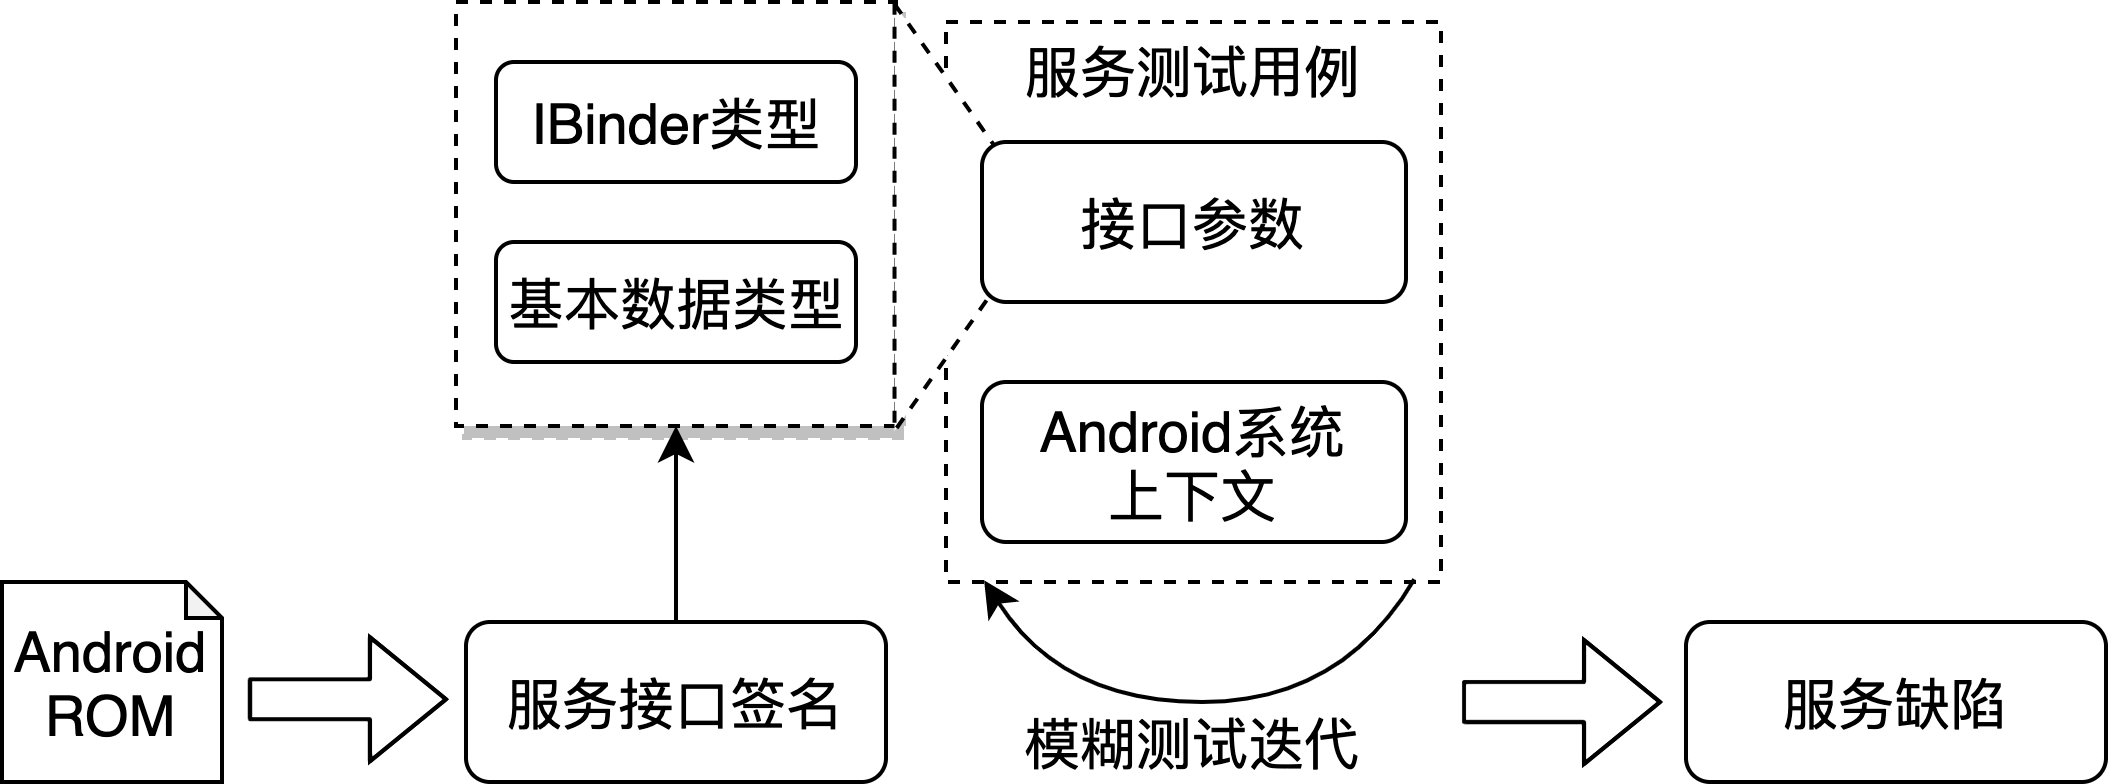
\includegraphics[width=\textwidth]{figure/overview.png}
	\caption{定制Android系统服务测试方法}
	\label{overview}
\end{figure}

本文提出的整套定制Android系统服务测试方法如图\ref{overview} 所示,研究内容主要包括:
\begin{itemize}
    \item 提出一种使用逆向工程自动化提取服务接口签名的方法,可从Java与Native服务的编译产物中,还原Binder通信序列化函数的结构特征,以推测出服务接口签名。
    \item 实现了一个服务模糊测试工具CASFuzzer:基于服务接口签名指导测试用例的生成与变异,提高模糊测试效率;通过Binder通信劫持技术,模拟影响服务执行的Android系统上下文,提高测试深度;动态地构造通用服务对象,以模拟Android中特有的IBinder类型的异常行为,更好地测试服务的边界情况。
    \item 在两个主流的定制Android系统上进行实验评估。实验结果表明,服务接口签名提取工具RevExtractor具有较高的准确性,服务模糊测试工具CASFuzzer中对Android系统上下文的模拟使得测试过程更加深入有效,测试用例中的异常IBinder类型可以触发特定的服务缺陷。
\end{itemize}



\section{本文组织结构}

本文组织如下:

第二章介绍了本文涉及到的背景知识与相关工作。首先介绍了Android系统及服务的相关背景知识;接着介绍了服务底层的Binder通信机制,包括其架构、通信流程以及通信协议;然后介绍了移动设备厂商如何定制Android系统以及这些定制化带来的安全隐患;最后介绍了Android组件间通信的相关工作。

第三章详细介绍了服务接口签名逆向提取工具RevExtractor,提取过程包含三个步骤:从Android ROM中提取服务相关编译产物;结合Android系统运行时状态,筛选出待测服务的通信序列化函数;从通信序列化函数的字节码与ARM汇编中,识别出序列化过程结构特征,以此推测出服务接口签名。

第四章详细介绍了服务模糊测试工具CASFuzzer:首先介绍测试用例中引入Android系统上下文的动机;接着介绍整体的服务模糊测试流程,包括如何启动待测服务;然后介绍测试用例生成策略,特别是对IBinder类型以及Android系统上下文这两种动态数据类型的模拟;最后介绍了如何评价测试用例,包括待测服务是否出现异常以及基本块覆盖率两个指标。

第五章是实验评估部分,对本文提出的服务接口签名逆向提取工具RevExtractor与服务模糊测试工具CASFuzzer进行了实验评估,验证了本文工作的有效性。

第六章是总结与展望,对本文工作进行简单的总结,并对未来可能的研究方向进行展望。

\chapter{背景知识}

本章首先介绍了Android系统架构,以及Android系统中的重要组成部分—服务。为了更好地理解服务的运行模式,接着介绍了服务底层的Binder通信机制,包括其架构、通信流程以及通信协议。然后介绍了第三方定制Android系统相关的背景,包括移动设备厂商如何定制Android系统以及这些定制所引入的安全问题。不少以往研究从Android组件间通信的角度对Android服务进行测试,最后介绍这个领域的相关研究进展。

\section{Android系统架构}

Android是Google公司专为移动设备开发的基于Linux内核的开源操作系统,与大多数软件系统一样,采用分层的系统架构。如图\ref{android-os-arch}
 所示,自下到上分别是Linux内核层、Android虚拟机及系统运行库、应用框架层、应用程序层,各层次的功能如下:
\begin{itemize}
	\item Android系统底层基于Linux内核,但与上游的Linux内核存在不少显著差异。由于大量性能和安全方面的改动造成的不兼容性,Google一直在Linux内核下游维护着单独的Android内核分支。Android内核中,除了包括Google引入的Binder、Ashmem、Logger等通用设备驱动以外,还包括各家移动设备厂商引入的诸如摄像机、屏幕、编解码器等定制硬件设备驱动。
	\item Android虚拟机是一个基于寄存器架构的虚拟机,运行Dalvik字节码,为应用提供运行环境并保证了不同应用间的隔离,自Android 5.0之后,原有的Dalvik虚拟机被ART虚拟机所替代,并结合AOT(Ahead Of Time)等编译技术提高运行速度;系统运行库以C/C++动态链接库的形式分发,以JNI的形式暴露给上层应用使用,负责连接应用框架层和Linux内核层。
	\item 应用框架层以Android SDK的形式提供给应用开发者一系列Java API,便于开发上层应用。
	\item 应用程序层是指手机用户日常接触到的诸如地图、相机、购物软件等移动应用程序,这些应用程序既包括手机厂商预装的系统级应用,也包括用户从第三方应用市场下载的应用。
\end{itemize}
\begin{figure}
	\centering
	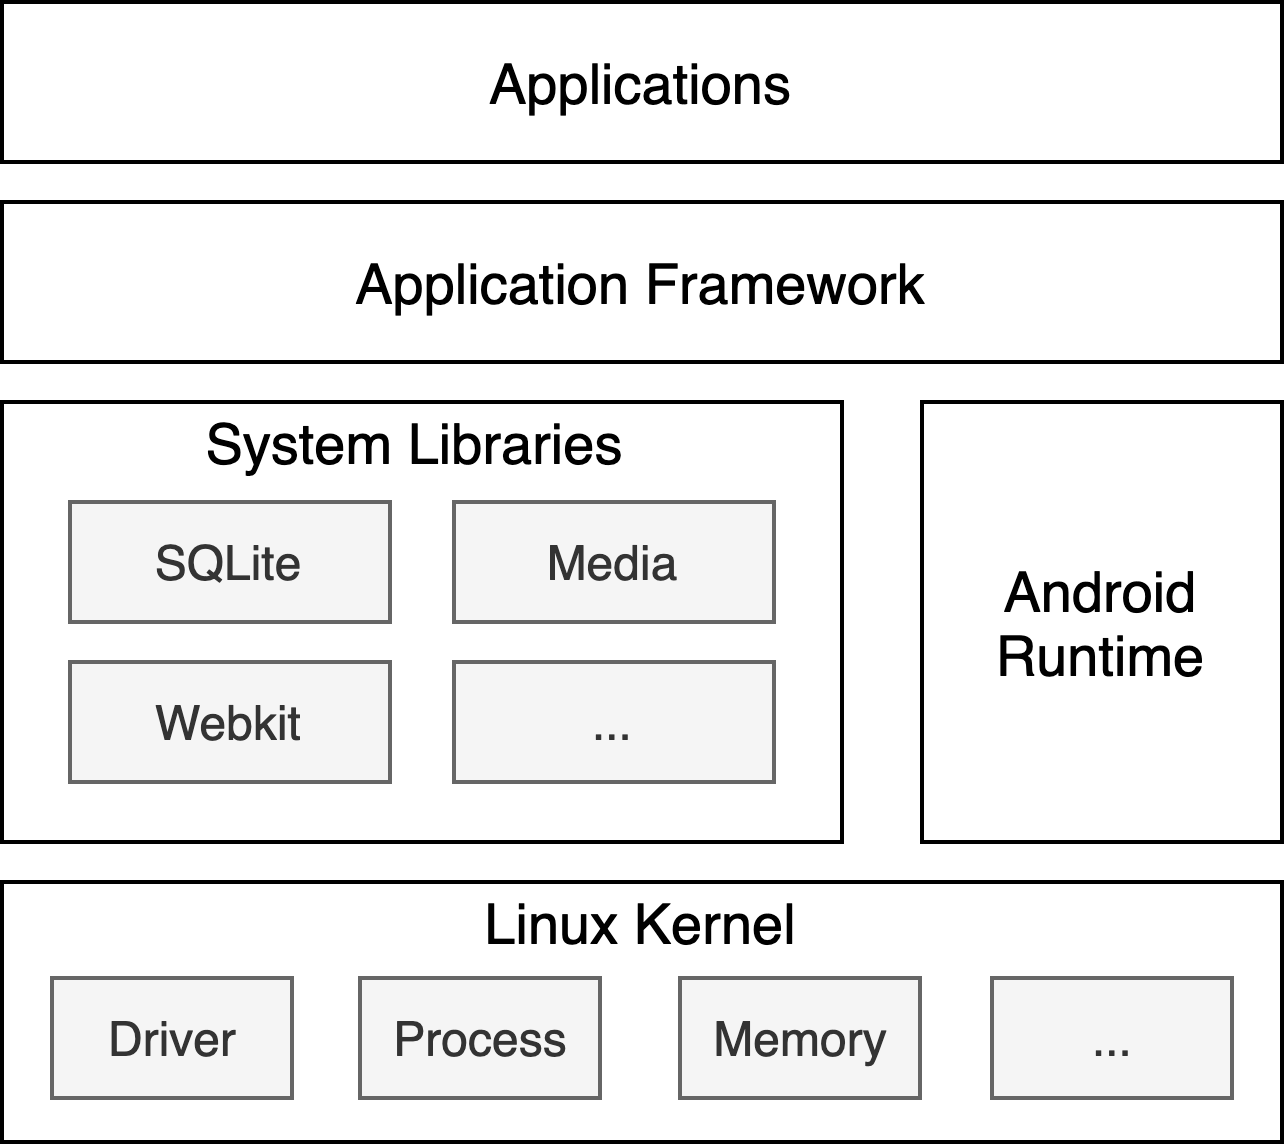
\includegraphics[width=.7\textwidth]{figure/2-background/android-os-arch.png}
	\caption{Android系统架构}
	\label{android-os-arch}
\end{figure}

Android框架定义了四大基本组件Activity,Service,BroadcastReceiver,ContentProvider:Activity负责组织图形用户界面,与用户进行交互;Service主要运行在后台,执行一些耗时逻辑,如播放音乐、执行文件I/O等等;BroadcastReceiver用来接收应用和系统发送的广播事件;ContentProvider提供不同应用间的数据共享功能。

\section{Android服务}

作为Android四大基本组件之一,服务是Android系统的核心组成部分。服务除了以组件的形式在Android应用中被广泛使用外,Android系统绝大多数的功能也是通过系统服务(System Service)的形式暴露给上层使用,如提供应用管理功能的PackageManager、提供网络连接管理功能的NetworkManagementService、管理摄像机的CameraService等等。

从服务的生命周期来看,可分为启动式服务(Started Service)和绑定式服务(Bound Service)两种类型\cite{service}。对于启动式服务来说,应用组件通过构造Intent对象,调用startService接口显式启动服务,启动式服务的生命周期独立于调用者,即使调用者被销毁,启动式服务也仍可继续运行。对于绑定式服务来说,应用组件通过bindService接口获得对应的服务IBinder对象,之后应用组件可通过该IBinder对象与绑定式服务进行交互,绑定式服务的生命周期依赖于应用组件,若应用组件被销毁,则绑定式服务也随之被Android系统所销毁。但这两者的关系也并不绝对,有些服务既可以是启动式服务,也同时提供了绑定接口,在绑定的应用组件被销毁之后,仍会继续运行。

从服务的可见性角度来看,可分为实名服务和匿名服务两类。实名服务的基本信息存储在Service Manager中,外部组件可通过服务名称从Service Manager中检索对应的服务引用,系统服务都属于实名服务;匿名服务只对调用者双方可见,服务对象存储在服务端进程的LoadApk对象之中,无法在Service Manager中检索到,例如应用中的绑定式服务就属于匿名服务。

服务底层通过Binder通信机制与其他应用组件发生交互,了解Binder通信机制有助于我们更好地分析服务的行为与运行状态。


\section{Binder通信机制}

Binder是Android系统特有的进程间通信机制,与Linux中常见的进程间通信机制(如Named Pipe、Message Queue、Signal、Share memory、Socket等方式)相比,Binder通信更为安全(支持对通信双方进行身份校验),数据传输也更为高效(只需要一次数据拷贝)。作为Android系统最基础的通信方式,Binder通信机制在Android系统的版本演化中很少变化,保证了上层应用在不同版本系统中的兼容性。


\subsection{Binder系统架构}

Binder系统架构如图\ref{binder-arch} 所示,在Binder通信系统中,所有可被访问的服务实体对应于一个内核空间中的IBinder对象,由服务端负责初始化,该对象将内部功能封装为一套自定义接口,就像类的成员函数。客户端持有这个IBinder对象的引用,通过该引用访问远程服务接口。由于IBinder对象实际存在于共享的内核空间中,打破了位于不同进程中用户态内存的隔离,使得客户端与服务端可以像对待本地对象一般,使用远程对象。

\begin{figure}
	\centering
	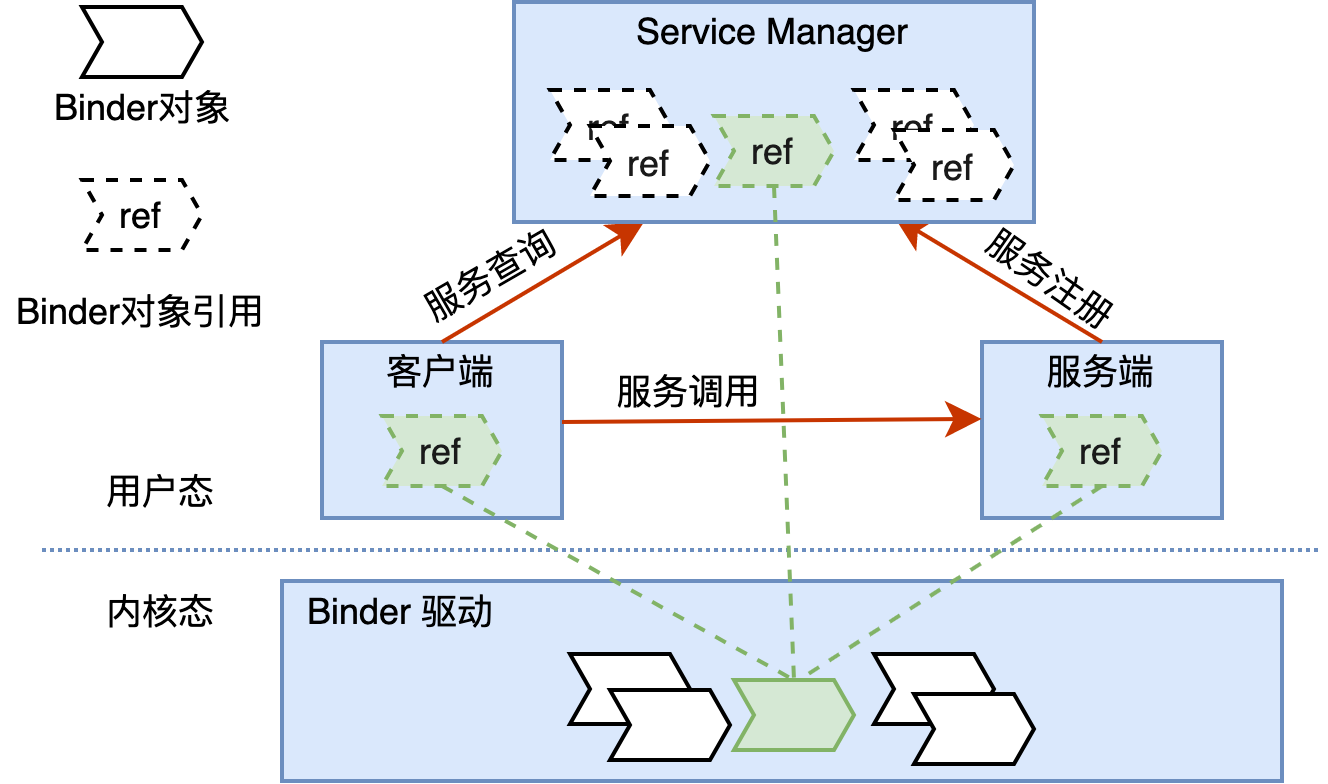
\includegraphics[width=\textwidth]{figure/2-background/binder-arch.png}
	\caption{Binder系统架构}
	\label{binder-arch}
\end{figure}

从组件的视角来看,Binder系统中除了客户端与服务端以外,还包括了管理各种服务的Service Manager,以及运行在内核态的Binder驱动。Service Manager是整个Binder系统中的管理者,对于实名服务来说,服务端初始化服务并注册到Service Manager中,客户端在通信前需要先从Service Manager中查询对应服务对象的引用。对Linux内核来说,Binder是一个特殊的字符型设备/dev/binder,内部实现遵循Linux设备驱动模型,提供open、close、mmap、ioctl系统调用,用户态的客户端、服务端与Service Manager通过上述系统调用与Binder驱动进行交互。

\subsection{AIDL接口}

为方便上层的Android应用开发者使用Binder机制进行跨进程通信,Android系统设计了一套通信接口定义语言AIDL \cite{aidl}(Android Interface Definition Language)。一个简单的AIDL接口示例如\ref{lst:aidl_example} 所示,其中IFoo服务内部包含doBar接口方法,Baz对象代表自定义Parcelable复杂结构体。

\begin{lstlisting}[caption={AIDL接口示例},label={lst:aidl_example}] 
import my.package.Baz;
interface IFoo {
    String doBar(int a, Baz obj);
}
\end{lstlisting}

Android编译工具链中包含AIDL代码生成工具,将AIDL接口定义转化为客户端与服务端均认可的编程接口(编程语言支持Java与C++),编程接口采用了经典的Proxy-Stub设计模式。应用开发者只需按照AIDL的语法规范描述服务接口,继承并实现自动生成的代理对象(Java中对应于ServiceProxy与ServiceStub对象;C++中对应于BpService与BnService对象),即可利用Binder机制实现跨进程通信。上层应用在通过AIDL接口进行通信时,就像进行本地函数调用一样方便,AIDL可以在Android任何进程之间使用,既可用于跨应用间的通信,也可用于Android系统服务间的通信。

\subsection{Binder通信流程}

\begin{figure}
	\centering
	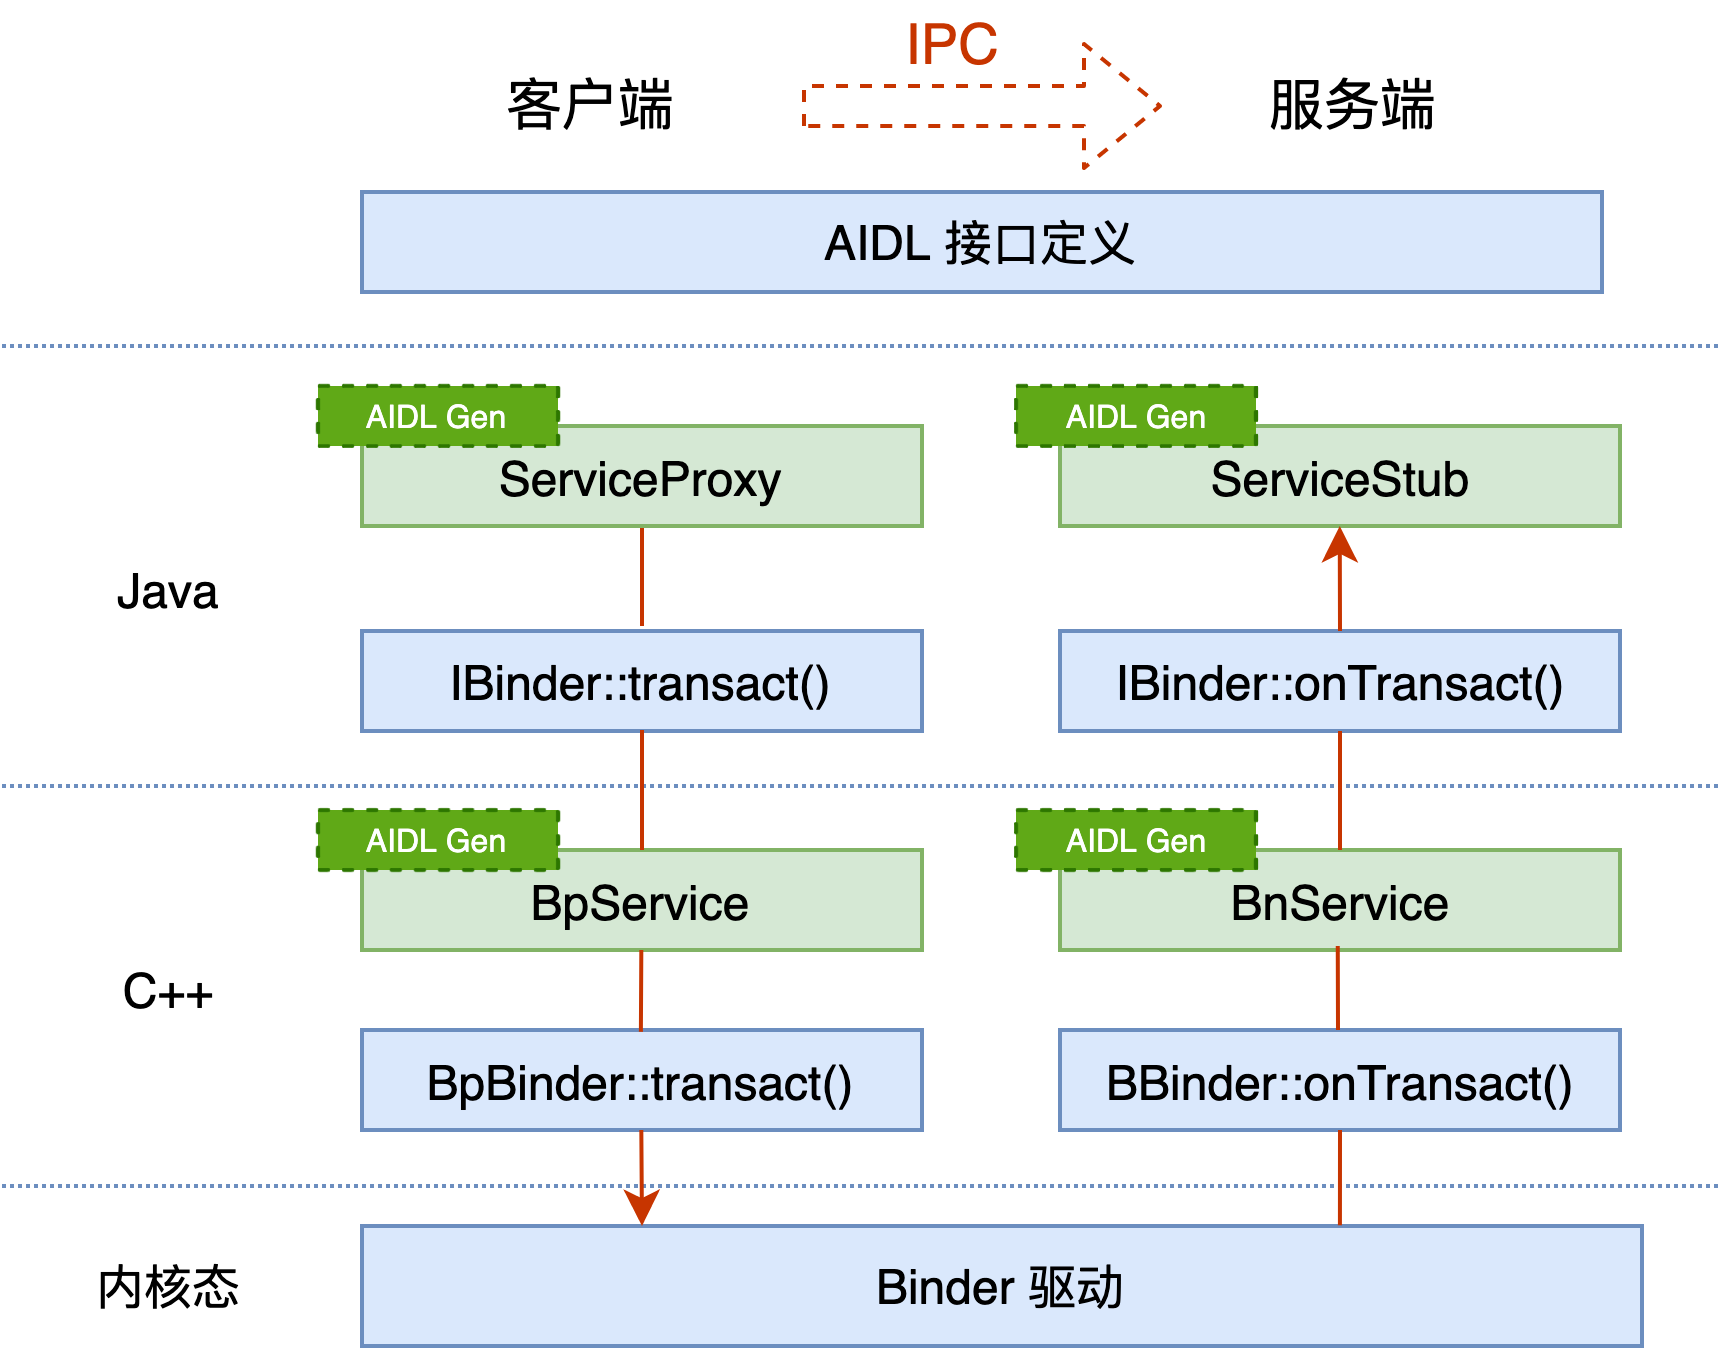
\includegraphics[width=.9\textwidth]{figure/2-background/binder-workflow.png}
	\caption{Binder通信流程}
	\label{binder-workflow}
\end{figure}

Binder通信流程如图\ref{binder-workflow} 所示:客户端的IPC请求通过Java层ServiceProxy对象与C++层的BpService对象,按照Binder通信协议序列化为Parcel数据,通过ioctl系统调用通知Binder驱动;Binder驱动根据服务对象索引,查询服务端所处进程号,通过ioctl系统调用通知服务端;服务端收到通知后,通过C++层的BnService对象与Java层的ServiceStub对象,将Parcel数据反序列化为相应接口的调用参数,调用真正的服务接口函数,函数的返回值也按照同样流程序列化并返回给客户端。

在Binder通信机制下,客户端与服务端既可以用Java实现,也可以用C++实现,不同编程语言间数据结构的兼容性由AIDL自动生成的序列化及反序列化层来保证。

\subsection{Binder通信协议}

传统的IPC方式在传输数据时,需要两次用户态与内核态间的数据拷贝:客户端将序列化的数据存放在发送缓冲区中,通过系统调用陷入内核态,内核中断处理例程使用copy\_from\_user函数将客户端进程中发送缓冲区的数据拷贝到内核空间;内核解析通信数据并查找到服务端所在进程,使用copy\_to\_user函数将内核空间的通信数据拷贝到服务端进程中的接收缓冲区。

Binder系统为提高数据传输效率,使用一种全新的策略,仅需一次用户态与内核态间的数据拷贝。Binder系统中,服务端利用mmap系统调用,从内核空间中直接映射出一片接收缓冲区,这块内存区域既可被服务端用户态进程直接访问,也被Binder内核驱动直接使用。当客户端向服务端传输数据时,Binder驱动会根据数据的大小,从映射出的缓冲区中找到大小合适的内存空间,使用copy\_from\_user函数将数据从发送缓冲区直接拷贝到接收缓冲区。

从内核驱动的角度来看,Binder客户端与服务端主要通过ioctl(fd, cmd, arg)系统调用进行交互,进一步可分为系统控制和数据传输两类交互请求:

\textbf{系统控制} \quad 对应的cmd参数为BINDER\_VERSION、BINDER\_SET\_CONTEXT\_MGR、BINDER\_SET\_MAX\_THREADS、BINDER\_THREAD\_EXIT。其交互请求的语义分别对应于:获得Binder驱动的版本号;将当前进程注册为Service Manager;服务端通过多线程的方式并发处理器客户端请求,客户端告知服务端所需的最大工作线程数,以避免资源的浪费;告知Binder驱动当前线程即将退出,Binder驱动清理内核对应的数据结构。

\textbf{数据传输} \quad 对应的cmd参数为BINDER\_WRITE\_READ。此时的arg参数指向binder\_write\_read结构体,结构体的内部格式如图\ref{binder-ioctl-data} 所示,分为两种情况:如果write\_size不为0就意为将数据写入Binder驱动;如果read\_size不为0就意为从Binder驱动读取数据。其中结构体内的write\_buffer和read\_buffer字段指向binder\_transaction\_data结构体数组,结构体中的code字段代表请求的目标服务接口编号,data.ptr.buffer字段指向Parcel序列化数据体。序列化数据体由policy传输模式、descriptor服务标识符、表示接口调用参数的flat\_binder\_object结构体数组构成。Binder驱动在用户态与内核态间拷贝flat\_binder\_object结构体时,会对结构体内部的字段进行修改,根据Binder服务端对象是否位于目标进程中,将其指向binder\_node(Binder实体)或binder\_ref(Binder引用)。

\begin{figure}
	\centering
	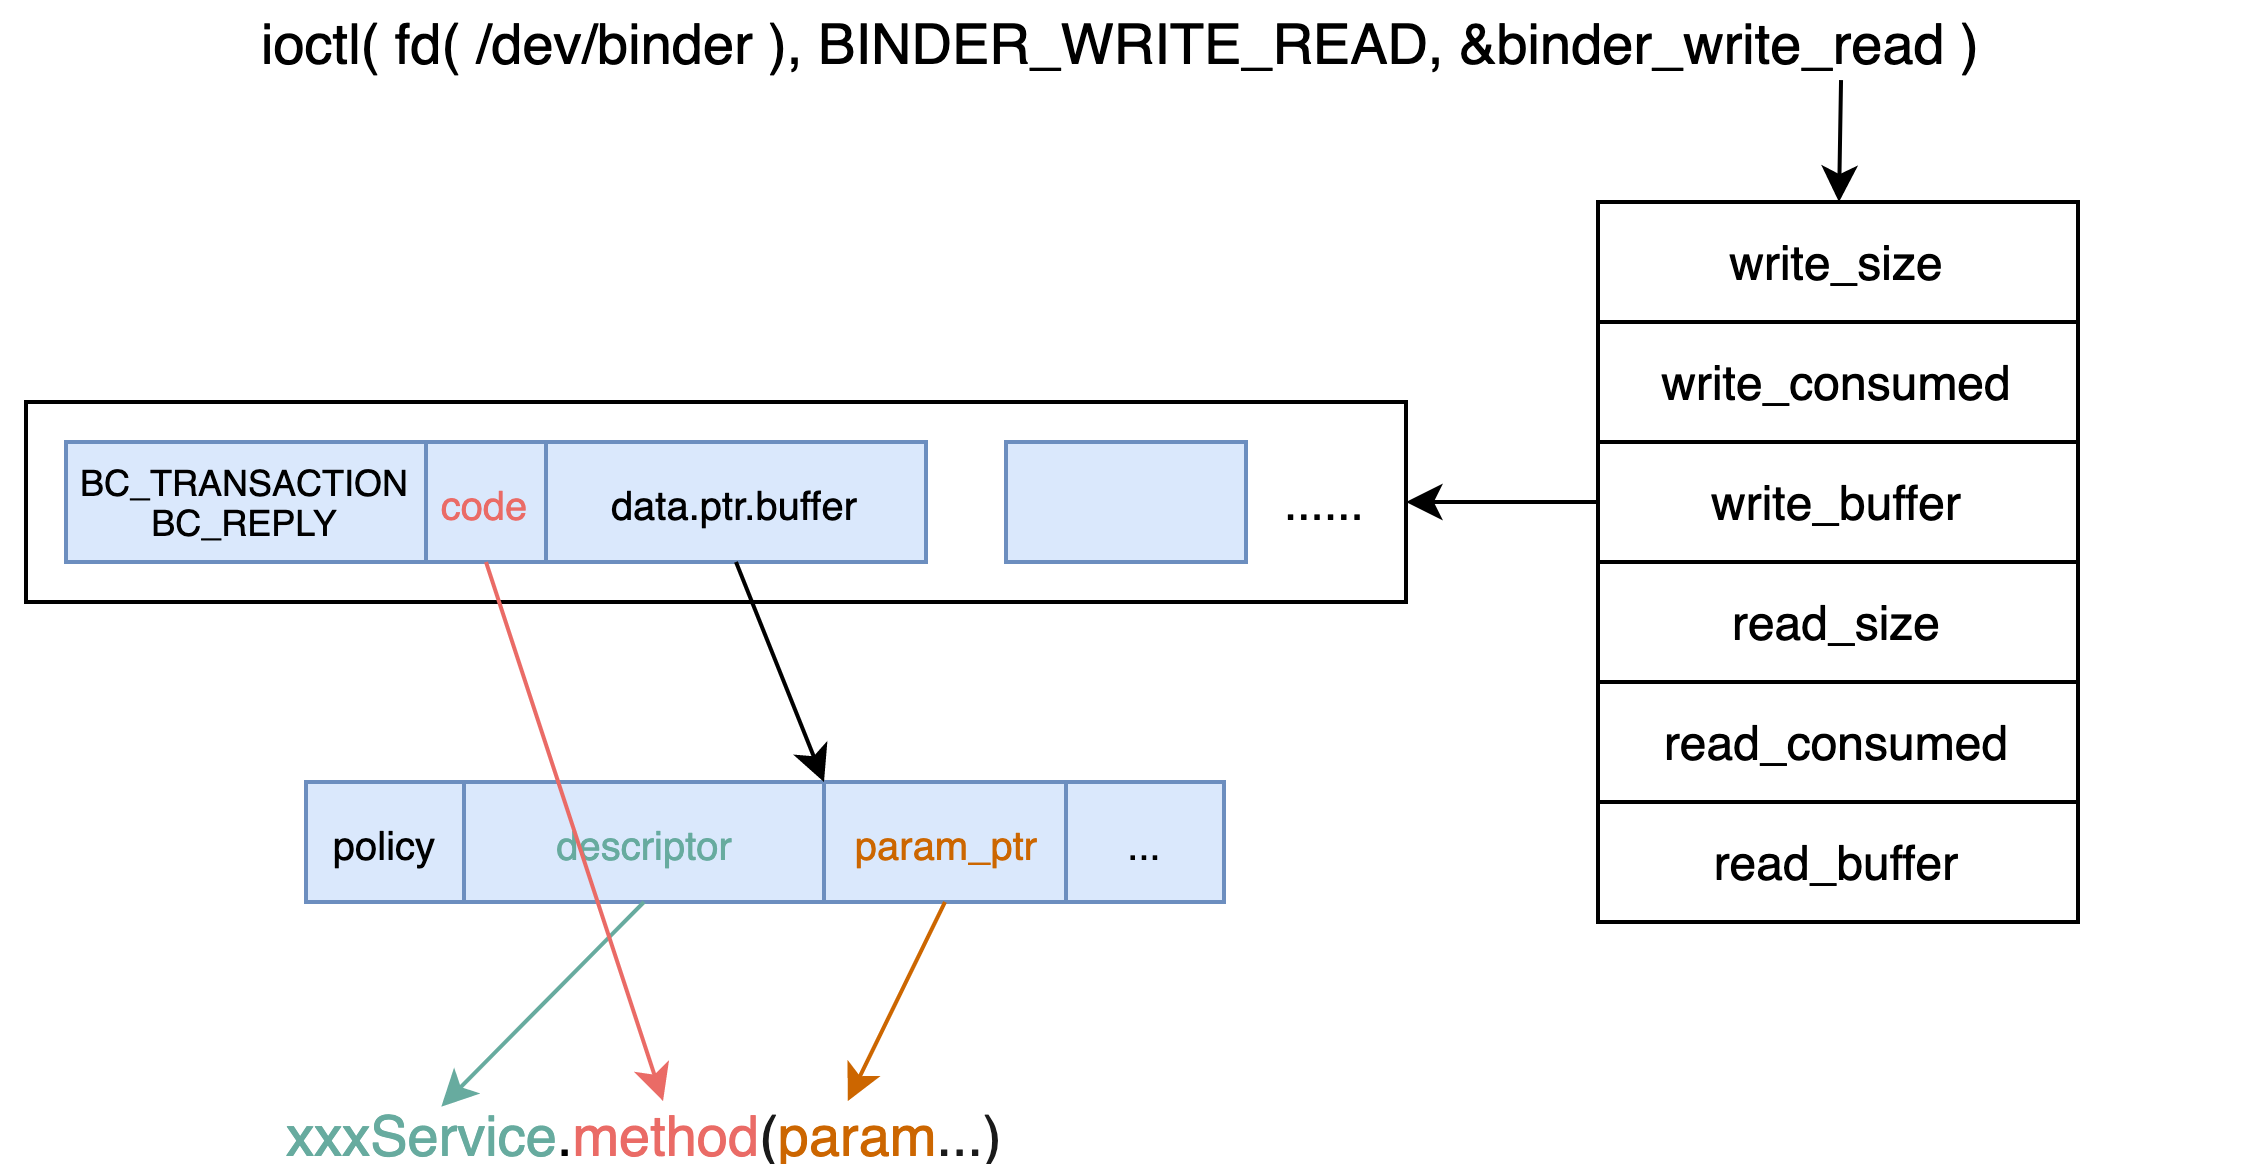
\includegraphics[width=\textwidth]{figure/2-background/binder-ioctl-data.png}
	\caption{Binder数据传输格式}
	\label{binder-ioctl-data}
\end{figure}

\section{定制Android系统}

由于Android系统的开放性,移动设备厂商往往会对Android系统进行深度的定制,以提供更丰富的功能。目前主流的移动设备厂商均推出了自己的定制Android系统,如小米的MIUI,华为的EMUI,三星的One UI等等,这些定制Android系统在设备出厂时就预装在手机上,系统的刷写包称为Android ROM。

与上游Google公司的AOSP相比,移动设备厂商对Android系统的定制化主要集中以下四个方面:

\textbf{Linux内核驱动} \quad 与PC或服务器不同,手机上的操作系统与设备自身的硬件有很强的绑定关系,上游Linux内核对硬件设备的支持不能满足移动设备快速迭代的需求。移动设备厂商为了支持更有竞争力的硬件配置(如高像素摄像机、高刷新率显示屏、AI加速处理器等),会在定制的Android内核中添加专用硬件设备驱动。

\textbf{Android应用框架} \quad Android系统在内核设备驱动之上添加了硬件抽象层,向下屏蔽驱动的实现细节,向上提供设备的统一访问接口,这些访问接口又被上层服务所组合,以AIDL接口的形式暴露给应用使用。为了适配新添加设备驱动的功能,移动设备厂商会对硬件抽象层与系统服务做修改,改变或拓展AOSP中的AIDL服务接口定义。

\textbf{权限配置} \quad Android系统在Linux基于UID与GID的安全机制之上,实现了Permission安全机制,支持更灵活的应用权限管理。Android应用框架通过系统中的配置文件(主要位于/system/etc/permissions等目录下)来完成应用权限管理系统的初始化,出于用户体验、管理便利性等方面的考虑,移动设备厂商会对这些权限配置文件进行修改。

\textbf{预装应用} \quad AOSP主要包含Android基础框架层以下的代码,Google公司将常见的应用(邮箱、地图、应用商店、浏览器等)打包成Google移动应用服务GMS单独出售。移动设备厂商基于性价比、产品竞争力、易用性等方面的考虑,往往会在定制Android系统中预装自家开发的一套系统应用,而不是选择GMS。具不完全统计\cite{gamba2020analysis},定制Android系统中80\%以上的应用来源于设备厂商或其他商业公司。


\subsection{安全隐患}

不少研究表明移动设备厂商对Android系统的定制化带来了不少额外的安全隐患:Zhou等人分析了2423个Android ROM中Linux设备驱动文件的访问权限配置,研究发现有1290个ROM中存在公开访问权限(比对应的AOSP中的文件访问权限更宽松)的设备驱动文件,并基于此成功构造了Touchscreen Keylogger、Screenshot Capture等隐私窃取攻击\cite{zhou2014peril};Yousra等人分析了591个Android ROM中对于应用权限的配置(UID/GID、应用包名、组件可见性、Permission等配置项),发现定制Android系统对这些配置项有较多的修改,并且修改后的权限配置很有可能导致安全漏洞\cite{aafer2016harvesting};Zhang等人分析了606个Android ROM中的应用卸载残留问题,通过静态分析的方式收集在应用安装与卸载过程中敏感信息的写入与删除,发现平均每个ROM中有106处应用卸载残留问题\cite{zhang2016hey}。

对于定制Android系统中的普遍存在的预装应用,Julien等人的研究\cite{gamba2020analysis}发现这些应用往往存在如下安全隐患:
\begin{itemize}
	\item 手机厂商定制的应用仅有少部分可以在公开的应用商店(如Google Play Store、Apkpure、酷安等)中获取到,使得这些定制应用被以往的安全研究工作所忽视。
	\item 相较于AOSP的权限配置,很多预装应用被赋予了过多的系统关键权限,这些应用本身的漏洞很有可能导致它们被攻击者所控制,进一步导致用户敏感信息的泄漏。
	\item 预装应用通过可暴露组件,将其资源和功能共享给其他应用使用,这些暴露组件在处理外部请求时如果没有对调用者权限进行校验,则很有可能被攻击者所利用。
	\item 这些预装应用中普遍存在收集个人隐私数据,追踪用户等行为。
\end{itemize}

\section{Android组件间通信问题研究}

Android系统及应用通过组件间通信(Inter-Component Communication,ICC)来实现组件的复用,这种机制使得Android应用趋向于低耦合高内聚的软件设计模式。由于用户往往会在设备上安装几十甚至上百个应用,在这样一个复杂的系统环境之中,恶意程序同样也可以利用组件间通信的方式,绕过Android系统的安全隔离机制,窃取用户敏感信息,执行非法指令等恶意行为。

不少研究从组件间通信的角度,对隐私泄漏、合谋攻击等漏洞进行挖掘。挖掘这类漏洞的挑战在于具有安全隐患的程序执行路径分散在各个应用之中,仅仅分析其中的一个应用无法检测出安全问题,需要从通信关键API的调用参数中还原出多个应用组件的调用关系。

已有工作主要以Intent为通信载体,研究组件间通信问题。Intent是一个由目标组件名称以及键值对形式的额外数据构成的消息对象。启动Activity、启动Service、广播消息等常见的Android应用管理功能皆是通过Intent来实现。

Chin等人第一个指出Intent存在的安全隐患,将基于Intent的攻击分为两类,Intent接受者未授权与恶意的Intent消息注入,并通过静态分析的方式检测Intent的内容是否安全\cite{chin2011analyzing}。

Intent Fuzzer \cite{sasnauskas2014intent}以Intent为测试用例,使用模糊测试的方法对手机上的预装及第三方应用组件进行测试,测试过程中触发了应用反复crash、甚至Android系统重启等漏洞。

FlowDroid \cite{arzt2014flowdroid}对单个应用利用静态分析的方式,生成虚拟的生命周期和回掉函数,以构造完整的程序调用图(CG)和过程间控制流程图(ICFG),追踪从source到sink的数据流,分析出敏感信息流的泄漏路径。

IccTA \cite{li2015iccta}利用字节码插桩技术修改应用,以构建跨应用间连续的控制流图,使用静态污点分析的方式,结合FlowDroid的方法,对跨应用的数据流进行追踪。


\chapter{服务接口签名逆向工程}

\begin{figure}
	\centering
	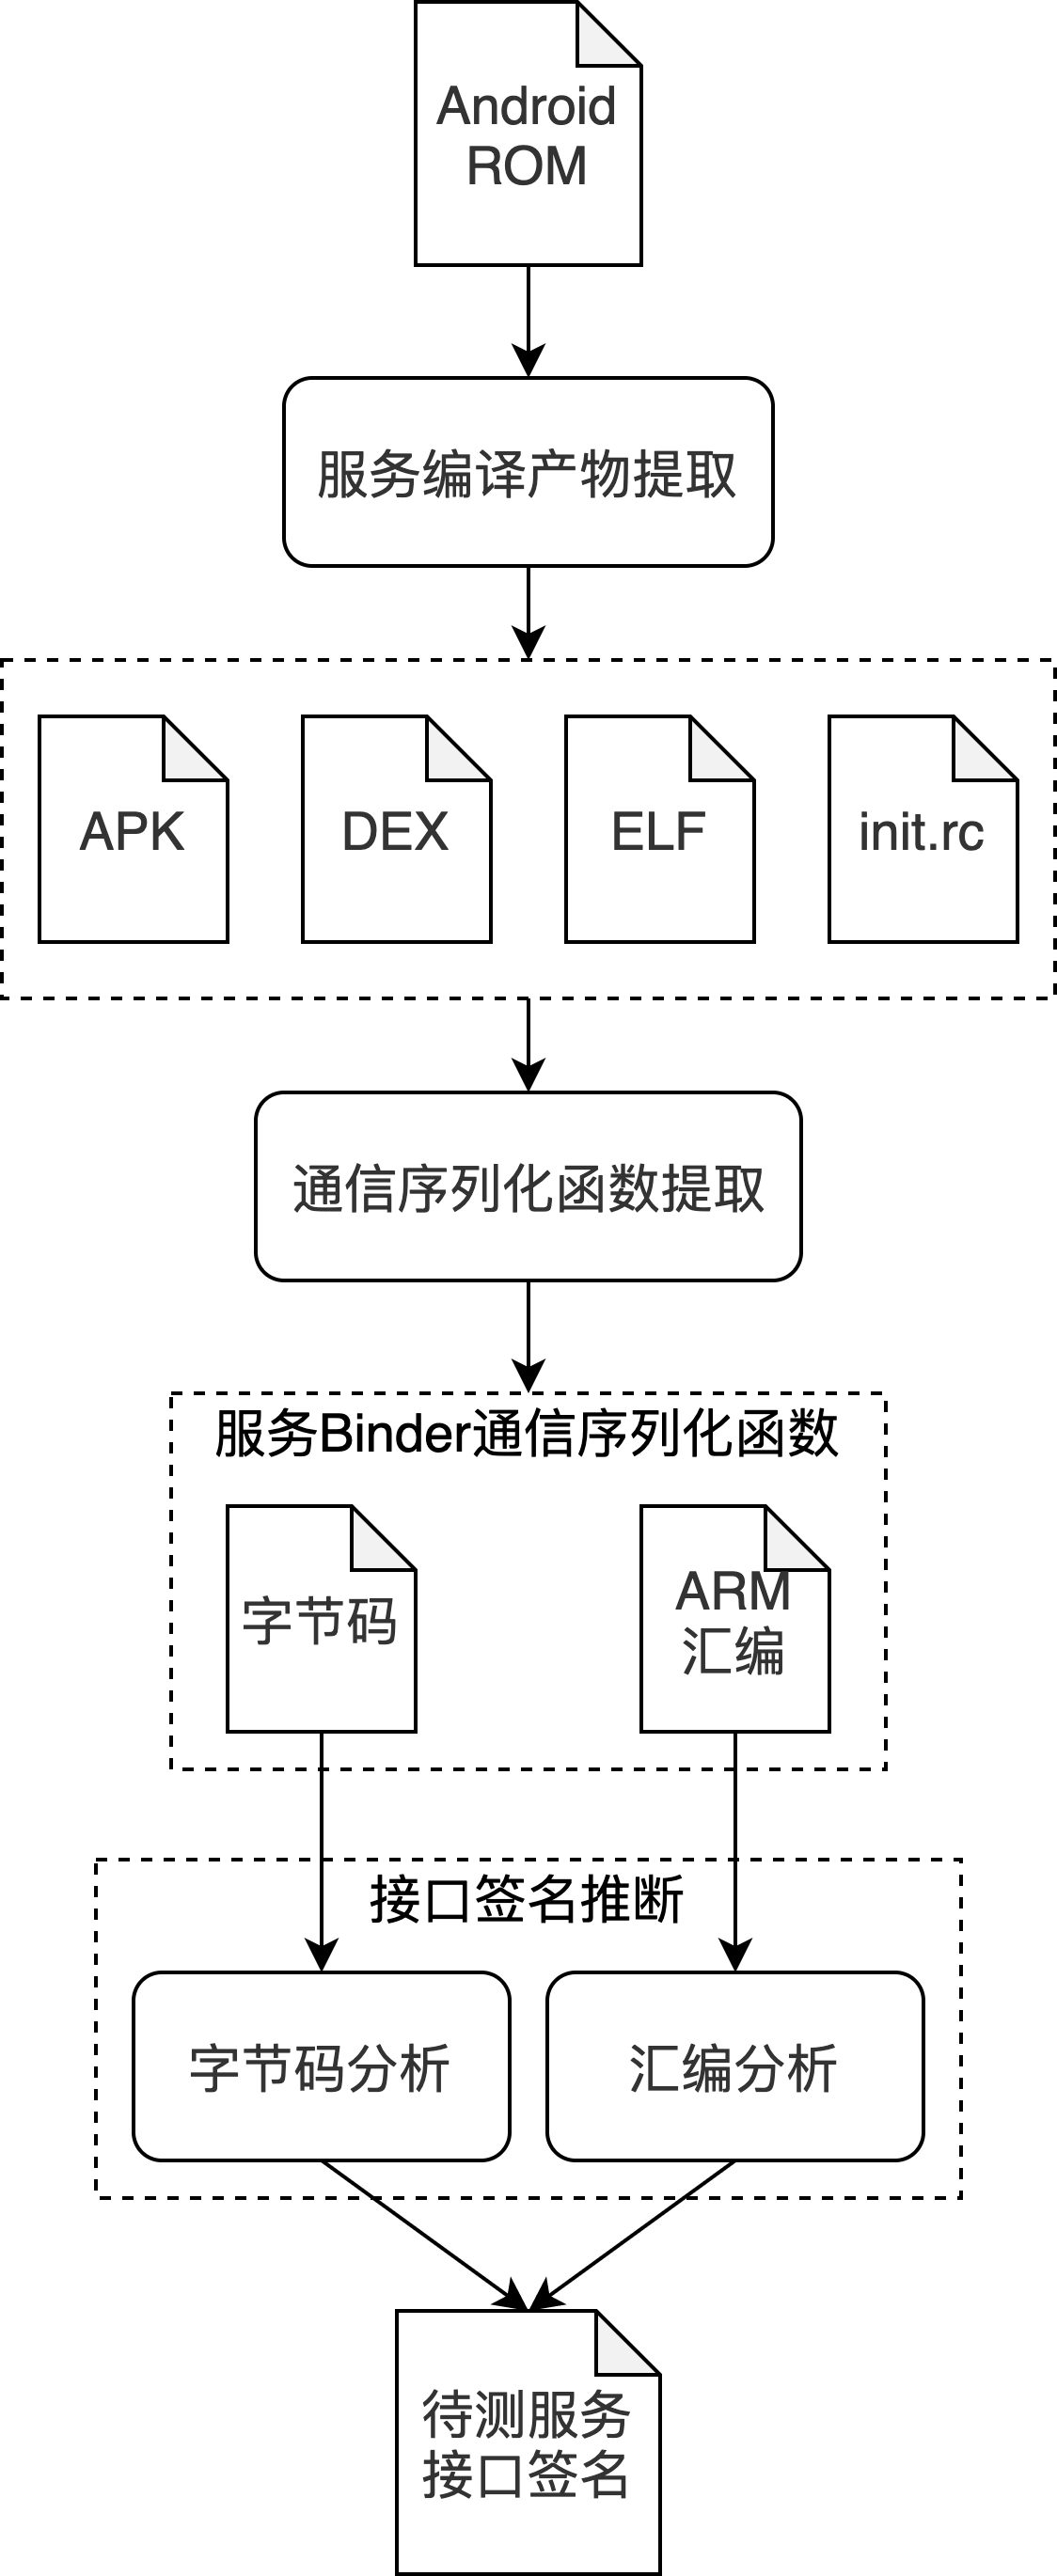
\includegraphics[width=0.5\textwidth]{figure/3-extractor/workflow-simple.png}
	\caption{闭源服务接口签名提取流程}
	\label{extractor-workflow}
\end{figure}

为了生成有效的服务接口测试用例,在对服务进行模糊测试前,我们需要先提取出服务的接口签名(包括接口编号、接口方法及返回值类型)。已有工作中对于服务接口签名的提取方法有如下三种:

\textbf{Binder通信数据监控} \quad BinderCracker \cite{feng2016bindercracker}在设备驱动的层次,收集Binder通信的底层数据,对该数据结构进行变异,重放该Binder通信数据对目标服务进行测试。属于黑盒的record-and-replay方法,测试效果很大程度依赖于预先记录通信数据的质量,容易漏过不常使用的接口,而且对通信数据的随机变异很难生成合法的服务接口调用参数,测试效率较低。

\textbf{Java反射} \quad 在Java层,通过Service Manager对象的getService方法,获取Java系统服务的类名,利用反射技术获取该Java类的方法签名。该方法效率高、实现简单且不依赖于源码,被不少灰盒测试工具\cite{iannillo2017chizpurfle}\cite{wu2017exception}所使用。但只能应用于Java服务,不能应用于不注册于Service Manager中的匿名应用服务。

\textbf{源代码静态分析} \quad 绝大多数服务的通信函数是通过AIDL代码生成工具自动生成的,Gu等人通过AOSP源码中的AIDL接口定义提取出服务接口签名\cite{gu2016exploiting}。为进一步提高接口类型模型的精度,FANS \cite{liu2020fans}通过Native服务C++源码的静态分析,根据变量类型与名称推测出不同接口间参数与返回值的依赖关系。从源码中提取的接口签名精度高,但不能应用于闭源服务之上。

上述方法要么在接口签名的提取精度上有缺陷,要么依赖于服务的源码,不能满足定制Android系统中闭源的Java与Native服务的测试需求。

我们发现服务接口签名与服务Binder通信序列化函数中的代码特征相对应,即使是在编译生成的字节码与ARM汇编代码中,这些代码结构特征也得到了一定程度的保留。只需从服务的编译产物中还原出这些代码结构特征,即可推测出服务接口签名。

对于定制Android系统中的预装应用服务、Java系统服务以及Native系统服务,这三类待测服务的接口签名提取流程如图\ref{extractor-workflow} 所示,包括服务编译产物提取、服务通信序列化函数提取、服务接口签名推断三个步骤。


\section{编译产物提取}

对不同类型服务进行逆向分析所需的编译产物不同,它们所处文件的提取规则如表\ref{tbl:service-artifact} 所示。

\begin{table}[!htbp]
	\centering
	\begin{tabular}{ccc}
		\toprule
		类型 & ROM中位置 & 文件格式 \\
		\toprule
		\multirow{4}*{应用服务} & /system/app & \multirow{4}*{APK} \\
		& /system/priv-app &  \\
		& /system/vendor &  \\
		& /system/preload & \\
		\hline
		\multirow{2}*{Java系统服务} & /system/framework & \multirow{2}*{JAR/odex/vdex} \\
		& /system/vendor/framework &  \\
		\hline
		\multirow{7}*{Native系统服务} & /system/lib & \multirow{5}*{ELF} \\
		& /system/lib64 &  \\
		& /system/vendor/lib &  \\
		& /system/vendor/lib64 &  \\
		\cline{2-3}
		& /system/etc/init & \multirow{2}*{rc}\\
		& /system/vendor/etc/init & \\
		\bottomrule
	\end{tabular}
	\caption{编译产物所处文件提取规则}
	\label{tbl:service-artifact}
\end{table}

Android ROM中预装应用的APK文件一般位于 /system/app等目录下,使用Apktool \cite{apktool}工具从中提取出包含应用配置的AndroidManifest.xml文件与包含Dalvik字节码的classes.dex文件。

Android系统为了将Java实现的系统服务暴露给其他应用使用,应用启动前会预先将依赖的Java对象加载到ART虚拟机的Class Loader中,相关的编译产物以JAR文件的形式位于 /system/framework等目录下。预加载Java对象配置信息保存在 /system/etc/preloaded-classes文件中,由Zygote孵化进程读取并加载。

\textbf{缺少DEX的情况} \quad 在Android 8.0之后,应用APK或 /system/framework下的JAR中一般不包含DEX文件,而是以odex文件(包含AOT编译过后的二进制码)与vdex文件(包含未压缩的Dalvik字节码以及加快验证速度的元信息)的形式存在,我们使用LIEF工具\cite{lief}从这些文件中还原回Dalvik字节码。

Android系统采用动态链接库的形式,将C++系统服务的接口暴露给其他程序使用,这些动态链接库文件一般位于 /system/lib等目录下,文件名形如"libxxxservice.so"。Native系统服务的配置信息则以Android初始化语言的形式记录在init.rc等文件之中,位于 /system/etc/init等目录下。

\section{通信序列化函数提取}

接下来,结合Android系统运行时状态,从上述编译产物中提取出待测服务通信序列化函数的字节码或汇编代码,分为两个步骤:
\begin{itemize}
	\item 确认待测服务,包括预装应用中暴露的绑定式服务,以及Java与Native系统服务;
	\item 根据服务的组件生命周期回调函数、序列化函数签名以及服务标识符等特征,提取待测服务的通信序列化函数。Java服务的通信序列化函数名为“Boolean onTransact(Integer code, Parcel data, Parcel reply, Integer flags)”,一般位于形如“XXXService\$Stub”的Java类中;Native服务的通信序列化函数名为“status\_t onTransact(uint32\_t code, const Parcel\& data, Parcel* reply, uint32\_t flags)”,一般位于形如“BnXXXService”的C++类中。
\end{itemize}

\subsection{应用服务}

\begin{lstlisting}[caption={应用服务的配置文件},label={lst:exorted_service},language=xml] 
<service android:name=".FooService" android:exported="true">
  <intent-filter>
    <action android:name="FOO_ACTION"/>
    <category android:name="FOO_CATEGORY"/>
  </intent-filter>
</service>
\end{lstlisting}

Android应用组件根据可见性可分为私有组件和公有组件(也叫暴露组件):私有组件只允许与同一应用中的组件,或者具有相同UID应用中的组件发生交互;暴露组件允许与其他应用程序发生交互,容易被其他恶意程序所利用,我们关注预装应用中的暴露服务组件。AndroidManifest文件中包含该应用的组件配置信息,文件格式如代码\ref{lst:exorted_service} 所示。从android:exported="true"属性即可确认为暴露服务;若该属性不存在,当存在至少一条intent-filter时则为暴露服务。


以往工作\cite{zhang2017systematically}\cite{yang2014intentfuzzer}主要关注以Intent为通信接口的启动式服务,忽略了以AIDL为通信接口的绑定式服务,我们关注预装应用中的绑定式服务。绑定式服务通过onBind(Intent)方法返回给调用者IBinder接口对象,之后调用者通过该接口对象与服务进行交互。从配置文件中的android:name属性确定服务类名,若该Java类实现了onBind方法,则为绑定式服务,通过数据流分析计算出onBind方法的返回值具体类型,服务序列化函数所在的Stub类一定是onBind方法返回值的父类。



\subsection{系统服务}

所有的系统服务都注册在Service Manager中,通过它的listService接口列举出系统服务名称与服务标识符descriptor。

每个服务必须实现一个返回值为descriptor的特殊接口,一般通过AIDL代码生成工具自动生成,因此根据服务序列化Stub类中的descriptor字符串值可确定该Stub类对应于哪一个服务。

绝大多数Java系统服务位于system\_server进程中,如BackupManagerService、PackageManagerService、PowerManagerService等等,每个服务以一个单独线程的形式运行。读取该进程的虚拟内存使用情况表 /proc/[pid]/maps,从该表的最后一列中筛选出该进程所加载的字节码文件(以jar、vdex、odex、oat为文件后缀名)。在这些字节码文件中根据序列化函数签名以及descriptor字符串两个特征,识别出该服务通信序列化函数所在的Stub类。

\begin{lstlisting}[caption={cameraserver.rc配置文件},label={lst:system_service_initrc}] 
service cameraserver /system/bin/cameraserver
  class main
  user cameraserver
  group audio camera input drmrpc
\end{lstlisting}

Native系统服务一般位于独立的守护进程之中,如cameraserver、mediaserver、audioserver等等。这些进程的启动参数以Android初始化语言(Android Init Language,AIL)的形式记录在init.rc等配置文件之中。以cameraserver为例,对应的配置文件如\ref{lst:system_service_initrc} 所示,从中可提取出进程可执行文件、UID、GID等服务启动配置信息。解析服务进程可执行文件在动态链接过程中所依赖的so库文件,在这些动态链接库文件的符号表中,先根据序列化函数签名筛选出所有服务对象的序列化函数,接着根据服务标识符descriptor在这些序列化函数的汇编代码中进行特征匹配,以确认服务与其通信序列化函数的对应关系。


我们通过拦截系统服务在Service Manager中的注册过程,以获得服务名称、所处进程PID、Binder驱动内的服务索引handle等运行时信息。Service Manager的服务端使用C/C++实现,在AOSP中服务注册过程的关键函数定义如代码\ref{lst:do_add_service} 所示。

\begin{lstlisting}[caption={服务注册函数定义},label={lst:do_add_service},language=C]
int do_add_service(struct binder_state *bs, 
                   // 服务名称
                   const uint16_t *s, size_t len, 
                   uint32_t handle, uid_t uid, 
                   int allow_isolated, pid_t spid);
\end{lstlisting}

拦截函数调用前需要知道函数在进程中的地址,由于do\_add\_service是一个内部的函数调用,它的地址并不会记录在进程可执行文件的符号表中。根据do\_add\_service函数的参数类型信息,并结合ARM中的函数调用规约(calling convention),我们可以生成出对应的汇编函数开场白(prologue)。由于定制Android系统很少对Service Manager实现进行修改,我们以汇编函数开场白为特征,扫描Service Manager服务端可执行文件,即可检索到do\_add\_service的函数地址。


\section{服务接口签名推断}

服务接口签名包括接口编号、接口方法参数以及返回值类型,这些信息都可对应于服务Binder通信序列化函数中的代码特征。即使是在编译过后的字节码与ARM汇编代码中,这些代码特征也得到了一定程度的保留,我们从编译产物中识别出这些代码特征,以推测服务接口签名。

\subsection{Binder通信序列化函数特征}

服务的Binder通信序列化onTransact函数结构如图\ref{ontransact-impl} 所示。函数的骨架是一个以code作为参数的switch-case,每个case分支实现了该服务某个接口的参数与返回值的序列化过程,code表示服务的接口编号,data表示接口请求参数的Parcel序列化数据对象,reply表示接口返回结果的Parcel序列化数据对象。switch-case代码结构中,以特殊常量0x5F4E5446为条件的分支中,将服务标识符descriptor写入reply中。通信序列化函数每个分支的序列化过程可进一步分为三段:
\begin{itemize}
	\item 从data中读取接口参数,对应于形如“readXXX”的反序列化API调用。
	\item 执行本地函数调用,若调用成功,则调用writeNoException函数标记成功,否则调用writeException函数写入异常信息,onTransact函数直接结束。
	\item 将调用结果写入reply中,对应于形如“writeXXX”的序列化API调用。
\end{itemize}

\begin{figure}
	\centering
	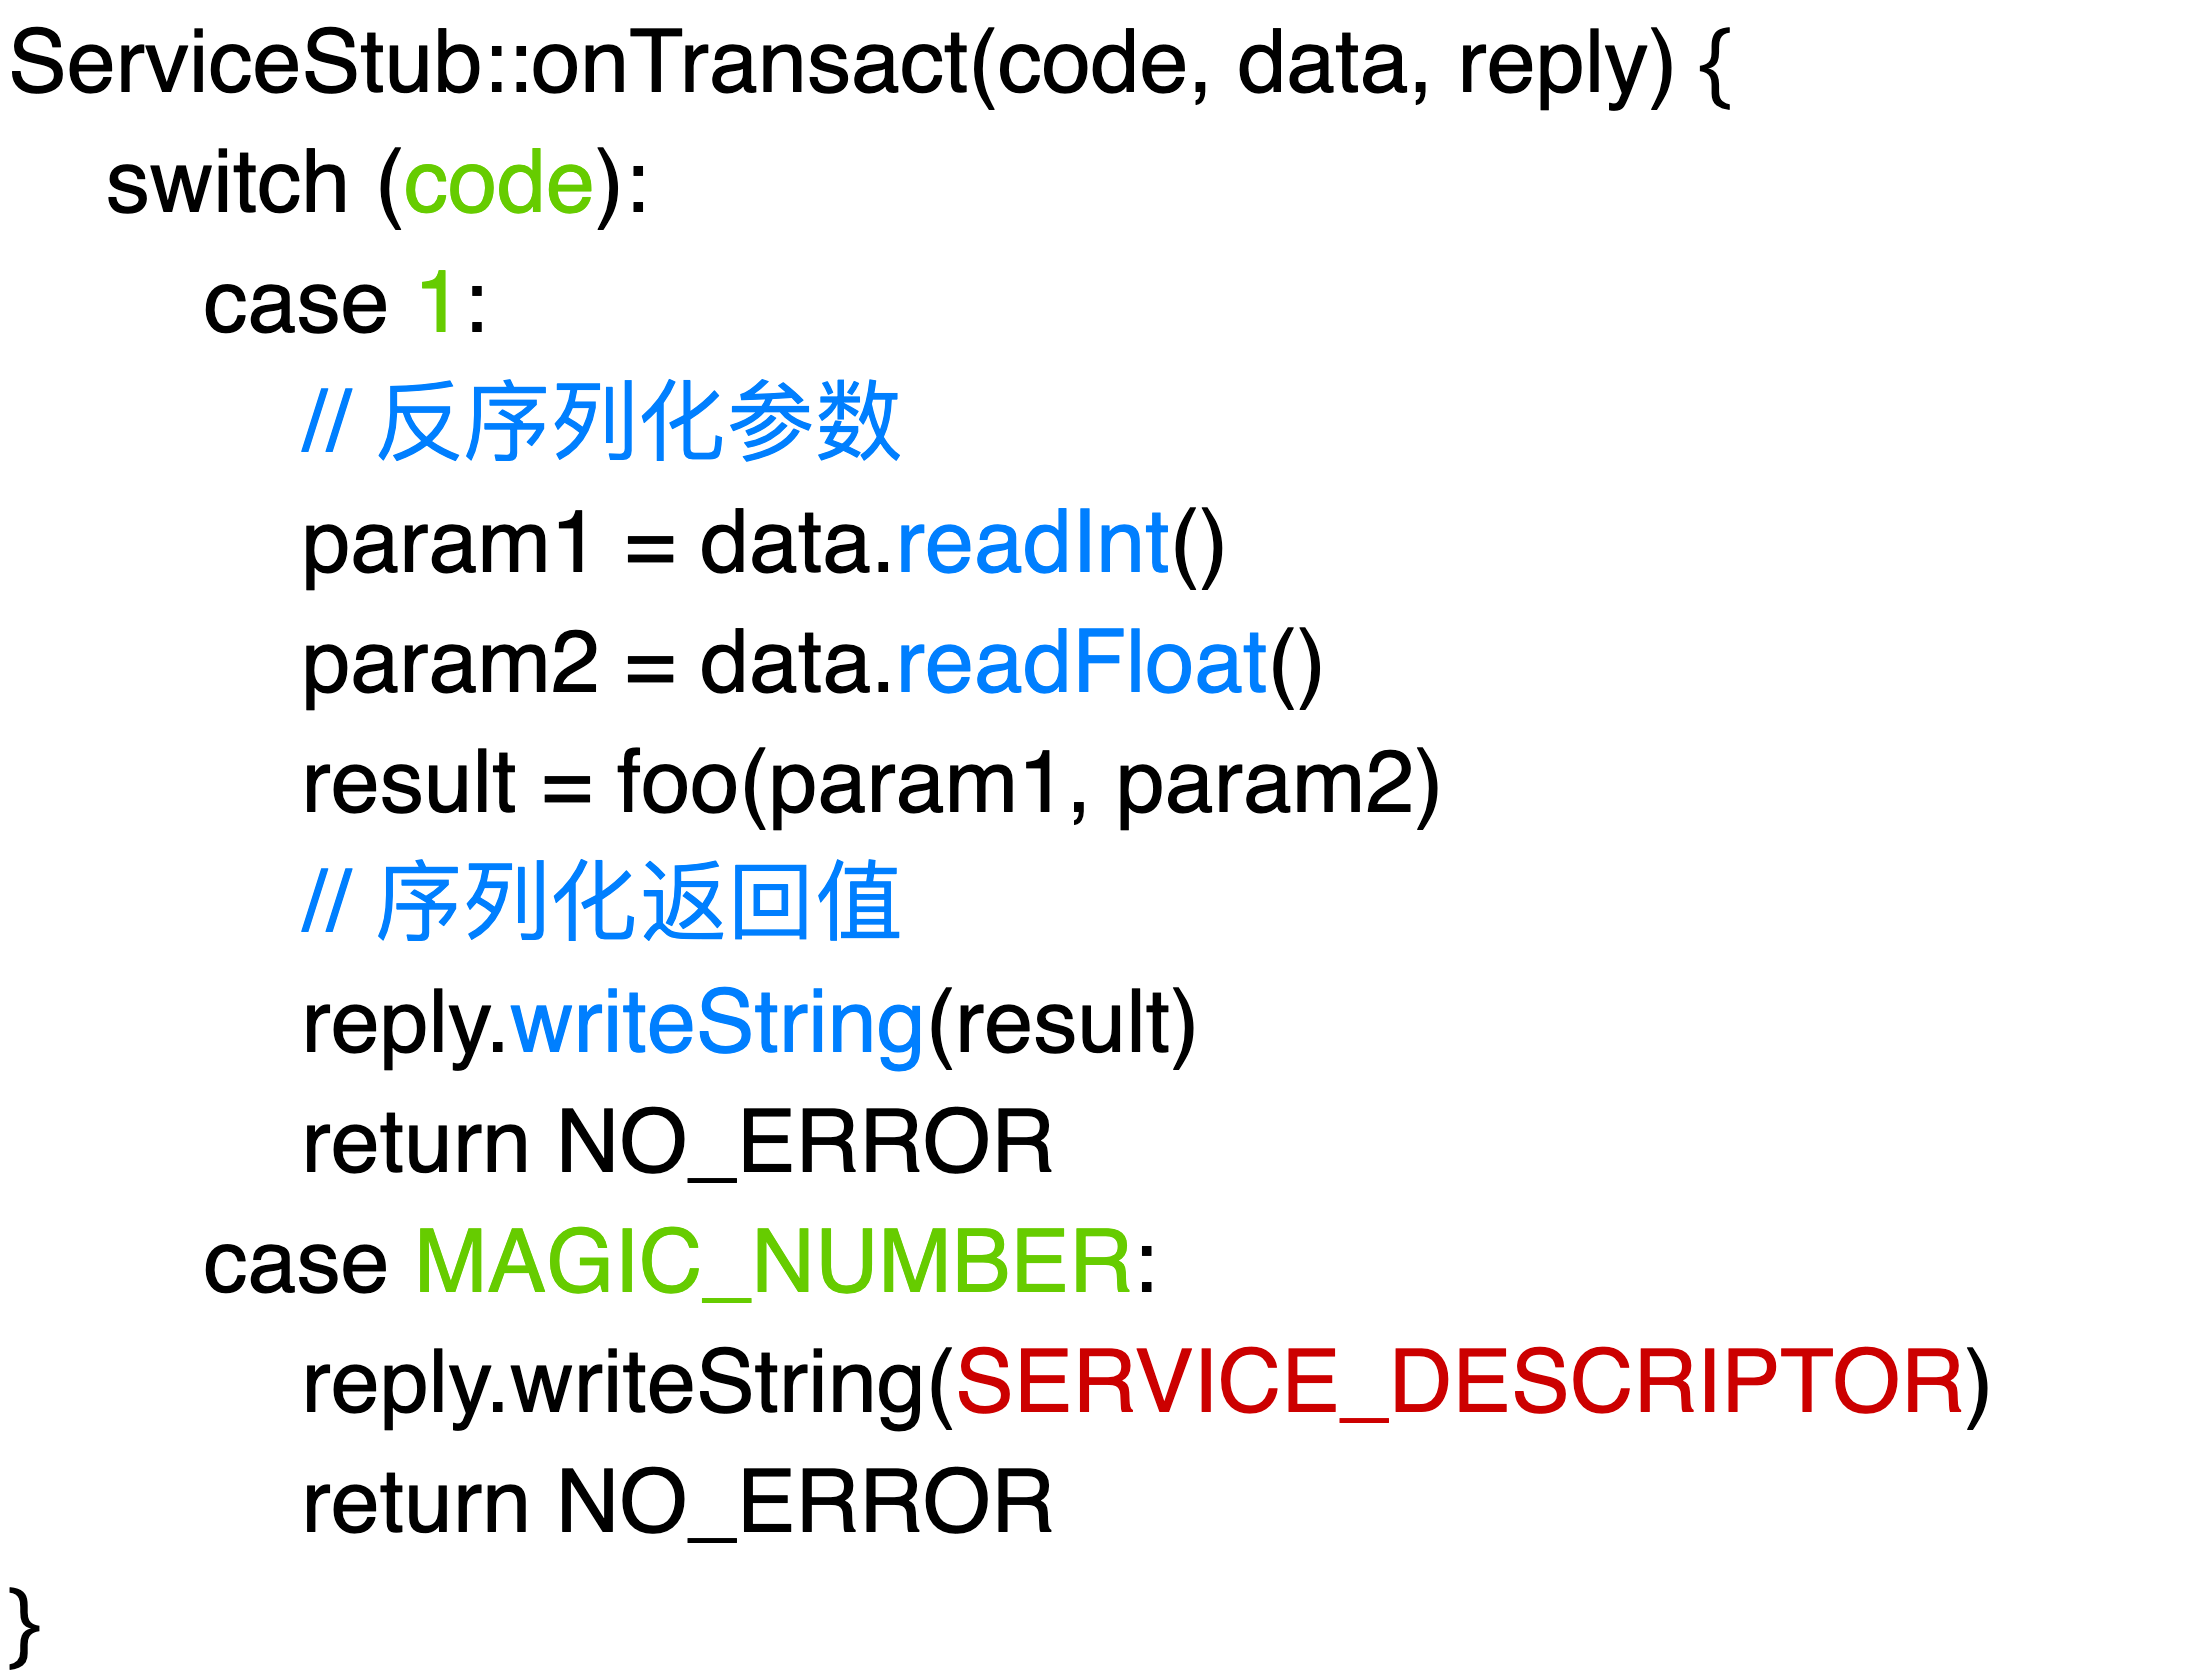
\includegraphics[width=0.7\textwidth]{figure/3-extractor/ontransact-impl.png}
	\caption{onTransact函数结构}
	\label{ontransact-impl}
\end{figure}

由于通信序列化过程代码往往由AIDL代码生成工具自动生成,结构较为稳定(事实上,即使是开发人员手工编写的通信序列化过程函数,也具有十分类似的代码结构)。即使是编译过后高度精简的二进制产物,也可从中识别出这些代码结构特征。


\if false
\begin{lstlisting}[caption={服务通信函数Java代码},label={lst:binder_transaction_java_example},language=java] 
public boolean onTransact(int code, 
                          android.os.Parcel data, 
                          android.os.Parcel reply, ...) {
  switch (code) {
    case TRANSACTION_FOO: {
      // 从Parcel中读取String,并检查descriptor是否匹配
      data.enforceInterface(descriptor);
      // 参数类型是int
      int _arg0 = data.readInt();
      java.lang.String _result = this.foo(_arg0);
      reply.writeNoException();
      // 函数调用的返回值类型为String
      reply.writeString(_result);
      return true;
    }
  }
}
\end{lstlisting}
\fi

\subsection{Parcel序列化API}

根据序列化数据类型的不同,可将Parcel序列化API分为六类:

\textbf{基本数据类型} \quad 包括readByte、readInt、readString等API。序列化数据的字节序由当前系统的处理器所决定。

\textbf{基本数据类型数组} \quad 包括readByteArray、readIntArray、readStringArray等API。Parcel序列化后的数组对象由开头表示数组大小的32位无符号整数与之后依次排列的数组项构成。为防止歧义,空对象会写入-1作为占位符。

\textbf{Bundle} \quad 包括readBundle、writeBundle等API。 Intent使用Bundle对象携带额外的信息,Bundle为键值对形式的Map,key固定为字符串类型。为防止歧义,空对象会写入-1作为占位符。

\textbf{Parcelable} \quad 包括readParcelable、createTypedArray等API。用于在进程间传输应用自定义的复杂结构体,这些复杂结构体需要实现自定义的序列化方法,Bundle对象也是一种特殊的Parcelable对象。当匹配到这类对象的序列化API时,我们需要递归地进入该对象的writeToParcel或readFromParcel函数实现中,重复以上所述的序列化API识别过程。

\textbf{FileDescriptor} \quad 包括readFileDescriptor和writeFileDescriptor这两个API。常常用于实现跨进程文件共享、套接字共享等功能,底层对应于Linux中的文件描述符。Parcel在序列化FileDescriptor对象时,将其转换为Binder内核驱动中的flat\_binder\_object对象,其定义如代码\ref{lst:flat_binder_object} 所示,并将type设置为BINDER\_TYPE\_FD,文件描述符存储在handler中。Binder驱动在传递文件描述符时,在目标进程中重新创建对应的文件描述符。

\textbf{IBinder} \quad 包括readStrongBinder、createBinderArray、createBinderList等API。IBinder对象本质是一种特殊的跨进程引用,是指向内核空间内Binder实体binder\_node的引用。Parcel在序列化IBinder对象时,将其转换为flat\_binder\_object对象,其中的type有四种可能的取值:
\begin{itemize}
	\item BINDER\_TYPE\_BINDER或BINDER\_TYPE\_WEAK\_BINDER:代表传输的是Binder实体,对应于Binder驱动内的binder\_node对象。当Binder驱动在传输flat\_binder\_object时,若发现其指向的binder\_node不存在,则在Binder驱动中创建并加入到binder\_proc所指向的红黑树之中。
	\item BINDER\_TYPE\_HANDLER或BINDER\_TYPE\_WEAK\_HANDLE:代表传输的是对Binder实体的引用,对应于Binder驱动内的binder\_ref对象。即使是指向同一个Binder实体的应用,不同进程的binder\_ref对象互相独立。因此Binder驱动在传输flat\_binder\_object时,需要修改handle以指向目标进程的binder\_ref对象,若binder\_ref对象不存在,则在目标进程中创建之。
\end{itemize}


\begin{lstlisting}[caption={flat\_binder\_object结构体定义},label={lst:flat_binder_object},language=C] 
struct binder_object_header {
  __u32 type;
};
struct flat_binder_object {
  struct binder_object_header hdr;
  __u32 flags;    // 传输方式
  union {
    __u64 binder; // 指向Binder驱动内binder_node结构对象的指针
    __u32 handle; // 指向Binder驱动内binder_ref结构对象的指针
  }
  __u64 cookie;   // 指向C++层BBinder对象的指针
};
\end{lstlisting}

\if false
\begin{table}[!htbp]
	\centering
	\begin{tabular}{ccc}
		\toprule
		AIDL类型 & Java类型 & C++类型 \\
		\toprule
		boolean & boolean & bool \\
		byte & byte & int8\_t \\
		char & char & char16\_t \\
		int & int & int32\_t \\
		long & long & int64\_t \\
		float & float & float \\
		double & double & double \\
		String & java.lang.String & android::String16 \\
		Parcelable & android.os.Parcelable & android::Parcelable \\
		IBinder & android.os.IBinder & android::IBinder \\
		T[] & T[] & std::vector<T> \\
		List<T> & java.Util.List<T> & std::vector<T> \\
		FileDescriptor & android.os.ParcelFileDescriptor & android::os::ParcelFileDescriptor \\ 
		\bottomrule
	\end{tabular}
	\caption{AIDL数据类型与不同编程语言中的对应关系}
	\label{tbl:aidl-type-mapping}
\end{table}
\fi

\subsection{从字节码中提取服务接口签名}

Java服务的编译产物为Dalvik字节码,我们借助Soot框架\cite{soot}将其转换为Jimple字节码,Jimple字节码的可读性较好,不难从中推测出服务接口签名:
\begin{itemize}
	\item Jimple字节码中通过lookupswitch指令与label标签来表示switch-case结构,lookupswitch指令中直接记录了相应分支的跳转条件。
	\item 在字节码中识别Parcel序列化API调用:对于staticinvoke、virtualinvoke方法调用指令,指令的参数直接包含目标函数签名,对应于基本数据类型及数组、Bundle、ParcelFileDescriptor、IBinder等数据的Parcel序列化API;对于interfaceinvoke接口调用指令,需要确定实现了该接口的实例对象类型,通过前向数据流分析找到该实例对象的构造函数调用,以确定实例对象的具体数据类型,对应于Parcelable复杂结构体的Parcel序列化API调用。
\end{itemize}


\if false
\begin{lstlisting}[caption={Java服务通信函数字节码},label={lst:transact_smali_example},basicstyle=\scriptsize]
.method public onTransact(ILandroid/os/Parcel;Landroid/os/Parcel;I)Z
  :sswitch_60
  // 验证descriptor
  invoke-virtual {p2, v6}, Landroid/os/Parcel;->enforceInterface(Ljava/lang/String;)V
  // 参数类型为int
  invoke-virtual/range {p2 .. p2}, Landroid/os/Parcel;->readInt()I
  
  invoke-virtual {p0, v2}, LFoo;->foo(I)Ljava/lang/String;
  move-result v3
  invoke-virtual/range {p3 .. p3}, Landroid/os/Parcel;->writeNoException()V
  
  // 返回值为String
  invoke-virtual {p3, v3}, Landroid/os/Parcel;->writeString(Ljava/lang/String;)V
  
  // return true
  const/4 v7, 0x1
  return v7

  .sparse-switch
    // 接口编码code为1
    0x1 -> :sswitch_60
  .end sparse-switch
.end method
\end{lstlisting}
\fi

\subsection{从ARM汇编中提取服务接口签名}

对于Native服务,从编译后生成的高度精简的ARM汇编中提取出上述特征有一定的挑战,即使是当前最先进的反编译工具RetDec \cite{retdec}与Hex-Rays \cite{hexrays},也仍然不能从汇编代码中完美还原回C++代码。由于汇编代码的可读性较差,推测服务接口签名的过程中有以下两点挑战:
\begin{itemize}
	\item \textbf{还原switch-case结构} \quad 服务通信序列化onTransact函数以switch-case为基本骨架,由于ARM汇编中不存在switch-case指令,分析的第一步需要将汇编代码块还原回源码中的switch-case结构。如果按传统方式将汇编函数体转化为控制流图(Control Flow Graph, CFG)来分析,会发现函数体所包含的基本块之间并不相连。
    \item \textbf{识别Parcel序列化API} \quad 在ARM汇编中,函数调用存在多种实现方式,对应于B、BL、BLR等分支跳转指令。静态函数、虚函数等不同类型的函数调用被编译后采用的寻址方式又不尽相同,这给从汇编中识别并解析出函数调用的语义带来了挑战。
\end{itemize}

\subsubsection{还原switch-case结构}

Android系统以Clang/LLVM为编译工具链,switch-case语句编译后对应于三种汇编代码结构:多重分支跳转、跳转表(jump table)、查找表(lookup table)。编译器根据分支跳转的效率以及汇编代码的大小决定生成哪种汇编代码结构。

对于通过AIDL代码生成工具生成的通信序列化onTransact函数来说,其中接口编码code为连续的枚举值。当分支跳转条件为连续的整型值时,Clang/LLVM会根据分支数量生成多重条件跳转或者
jump table汇编代码结构:分支数小于4时,生成前者,否则生成后者。

\textbf{多重分支跳转} \quad 组合多个分支跳转语句来表示switch-case的多个分支。每一个分支的开头指令满足如下特征:
\begin{itemize}
	\item 首先是CMP指令,比较接口编号code所处寄存器与常数是否相等;
    \item 接着是条件跳转指令,基于之前CMP指令的比较结果,跳转到对应分支的起始指令或下一条CMP指令,如B.EQ、B.NE等指令。
\end{itemize}

\textbf{jump table} \quad jump table实际上是一个以地址长度为宽度,以case数量为长度的数组,一般位于ELF的.rodata部分(对于ARM32指令集,会将jump table内嵌在函数体的汇编代码段中)。对于switch-case结构生成的jump table来说,其中表项存储了case分支开头指令的地址与表的基址之差,将表项与表基址相加即可计算出case分支的起始指令地址。

为了从.rodata中提取出jump table,我们还需要从汇编代码中提取出jump table的长度与基址两个属性:
\begin{itemize}
	\item switch-case结构中的default分支,对应的汇编形如代码\ref{lst:jump_table_aarch64} 的1-7行所示,由于接口编码code是从1开始递增的枚举型整数,因此default分支的判断条件为code是否大于该枚举类型的最大值,这个最大值也就是jump table的长度。
	\item 汇编通过间接寻址的方式使用jump table,如代码\ref{lst:jump_table_aarch64} 的9-16行所示,其中10-11行计算出了jump table的基址,对应计算公式为"(ADRP基址 >> 12) << 12 + 0x17000 + 0x700",0x17000代表.rodata基址相对当前代码页的偏移量,0x700代表jump table基址相对.rodata基址的偏移量。
\end{itemize}

\begin{lstlisting}[caption={AArch64汇编中对于jump table的使用},label={lst:jump_table_aarch64}] 
// W1寄存器中存储了onTransct的code参数值
SUB        W8, W1, #0x1
// 对应于switch-case中的default分支
// W8寄存器值无符号大于或等于25时,跳转到default分支
// 由此可推断出这个switch-case结构的分支数量的25
CMP        W8, #0x19
B.HI       45810
...
// X9寄存器中为jump table基址
ADRP       X9, 0x17000
ADD        X9, X9, 0x700
// X8寄存器中为对应表项的内容
LDRSW      X8, [X9, X8 LSL 0x2]
ADD        X8, X8, X9
// X8中存放了case分支的指令地址
BR         X8
\end{lstlisting}

\subsubsection{识别Parcel序列化API}

ARM汇编中,通过B、BL、BLR等分支跳转指令来表示函数调用,根据跳转指令的寻址方式,我们将函数调用分为两类:

\textbf{直接函数调用} \quad 指令的参数中包含目标函数地址,根据地址直接在符号表中查询即可知道对应的函数名。对于基本数据类型、基本数据类型数组、Bundle对象、ParcelFileDescriptor对象、IBinder对象这五类Parcel序列化API调用都属于这种情况。代码\ref{lst:identify_parcel_api_aarch64} 中的第5、20行皆属于直接函数调用。

\textbf{间接函数调用} \quad 指令的参数不直接包含目标函数地址,需要先通过运算将地址保存在寄存器中。最典型的例子就是C++中虚函数的调用,如代码\ref{lst:identify_parcel_api_aarch64} 的10-17行所示。Parcelable复杂对象的序列化接口writeToParcel与readFromParcel在基类中定义为虚函数,属于间接函数调用。识别间接函数调用的挑战在于如何计算出目标函数地址,本文参考VTint \cite{zhang2015vtint}中的方法,并将其从x86移植到ARM上,从汇编中识别虚函数调用,并确定对应的Parcel序列化API:
\begin{itemize}
	\item 识别构造函数调用;
	\item 在构造函数中,会进行虚函数表的初始化,以此特征可从构造函数中识别出该对象的虚函数表基址;
	\item 根据与虚函数表基址的偏移量计算出实际的函数调用地址;
	\item 以该地址为检索条件,从符号表中查询出目标函数签名;
\end{itemize}

\begin{lstlisting}[caption={Parcel序列化过程AArch64汇编},label={lst:identify_parcel_api_aarch64}] 
// X19寄存器里为this指针
// 将this指针转换为指向IBinder对象的指针
ADD        X1, X19, 8
MOV        X0, X21
BL         0x3b5f8 // android::Parcel::checkInterface
// 若checkInterface返回值为0,则跳转到onTransact函数结束
TBZ        W0, 0, 0x45dd4

// X8寄存器里为虚函数表的地址
LDR        X8, [X19]
MOV        X0, X19
// 将虚函数表中的表项值保存到X9寄存器
// X9寄存器实际指向了同一类下的成员函数地址
LDR        X9, [X8, 0xc0]
ADD        X8, SP, 8
BLR        X9
ADD        X1, SP, 8

MOV        X0, X20
BL         0x3b658 // android::Parcel::writeString8
\end{lstlisting}

由于Parcel序列化API的实现统一位于动态链接库libbinder中,为了实现运行时的动态链接,所以编译时一定会保留这些函数的符号信息。

\section{工具实现}

按照上述方法实现了服务接口签名逆向提取工具RevExtractor。工具中包含文件提取、字节码分析、汇编逆向分析、运行时配置信息提取四个主要模块:

\textbf{文件提取} \quad 使用Python代码实现。所有的服务相关文件都位于system分区下,对应于Android ROM中的system.img,可能会以两种形式存在:完整的ext4分区镜像,直接使用mount命令挂载即可;稀疏镜像(sparse image \cite{sparse_img}),是Android中特有的稀疏表示的分区镜像,镜像中去除了为零的填充数据,使用simg2img工具将其转化为完整的ext4分区镜像。

\textbf{字节码分析} \quad 先使用dex2jar \cite{dex2jar}工具,将dex文件转换为Jar文件,之后借助Soot框架\cite{soot}将Dalvik字节码转换为Jimple字节码进行分析,主要以Java代码实现。

\textbf{汇编逆向分析} \quad 借助Miasm框架\cite{miasm}以Python代码实现,由于Android系统可同时支持ARM32与ARM64两种指令集,对于这两种情况需要分别进行处理。

\textbf{运行时配置信息提取} \quad 其中的函数调用拦截部分借助Frida框架\cite{frida}以Javascript代码实现,其余以Python代码实现。

\section{本章小结}

本章介绍了服务接口签名逆向提取方法。首先介绍了已有工作中提取服务接口签名的方法,以及这些方法为何不适用于闭源的Java与Native服务。然后介绍了服务接口签名逆向工程的基本思路及工作流程,包括三个步骤:APK、DEX、ELF等服务编译产物的提取;结合Android系统运行时状态,根据服务配置、服务标识符等特征,提取出服务的通信序列化函数;从服务的编译产物中,识别出switch-case、序列化API调用等代码特征,以此推测出服务接口签名。最后综合以上方法,实现了服务接口签名逆向提取工具RevExtractor。


\chapter{系统上下文感知的服务模糊测试工具}

观察Android服务的内部实现逻辑,我们可以发现如下特征,如代码\ref{lst:service_api_impl_example} 所示:在执行真正的业务逻辑之前,需要对调用者权限、系统能耗模式等Android系统上下文进行检查,如果检查不通过,服务接口调用就提前结束。

\begin{lstlisting}[caption={服务实现中对Android系统上下文的检查},label={lst:service_api_impl_example},language=java,basicstyle=\footnotesize]
// 检查调用者是否有权限,PMS代表PackageManagerService
if(PMS.checkUidPermission(...) != PERMISSION_GRANTED) {
  return false;
}
// 检查调用者是否活跃,USS代表UsageStatsService
if (USS.isAppInactive(...)) {
  return false;
}
// 检查节能模式下是否允许执行,DIC代表DeviceIdleController
if (!DIC.isPowerSaveWhitelistApp(...)) {
  return false;
}

BUG();
\end{lstlisting}

然而,这些Android系统上下文往往与接口的输入参数无关,如果这些检查不通过的话,那么无论怎么生成输入参数,这个接口的测试深度都不会有太大变化,无法测试到真正有问题的代码。因此,对于服务接口的测试中,除了生成接口输入参数以外,还需要考虑Android系统的上下文。

实际上,这些对Android系统上下文的检查往往都是通过外部服务的接口调用来实现的,可以对这些接口调用进行劫持以模拟Android系统上下文。我们在Binder IPC层面统一地对这些外部服务接口调用进行劫持,以模拟Android系统上下文。

我们基于Binder IPC劫持、动态二进制插桩等技术,以服务接口签名指导测试用例的生成与变异,实现了一个系统上下文感知的Android服务模糊测试工具CASFuzzer(Context-Aware Service Fuzzer)。


\section{服务模糊测试流程}


\begin{figure}
	\centering
	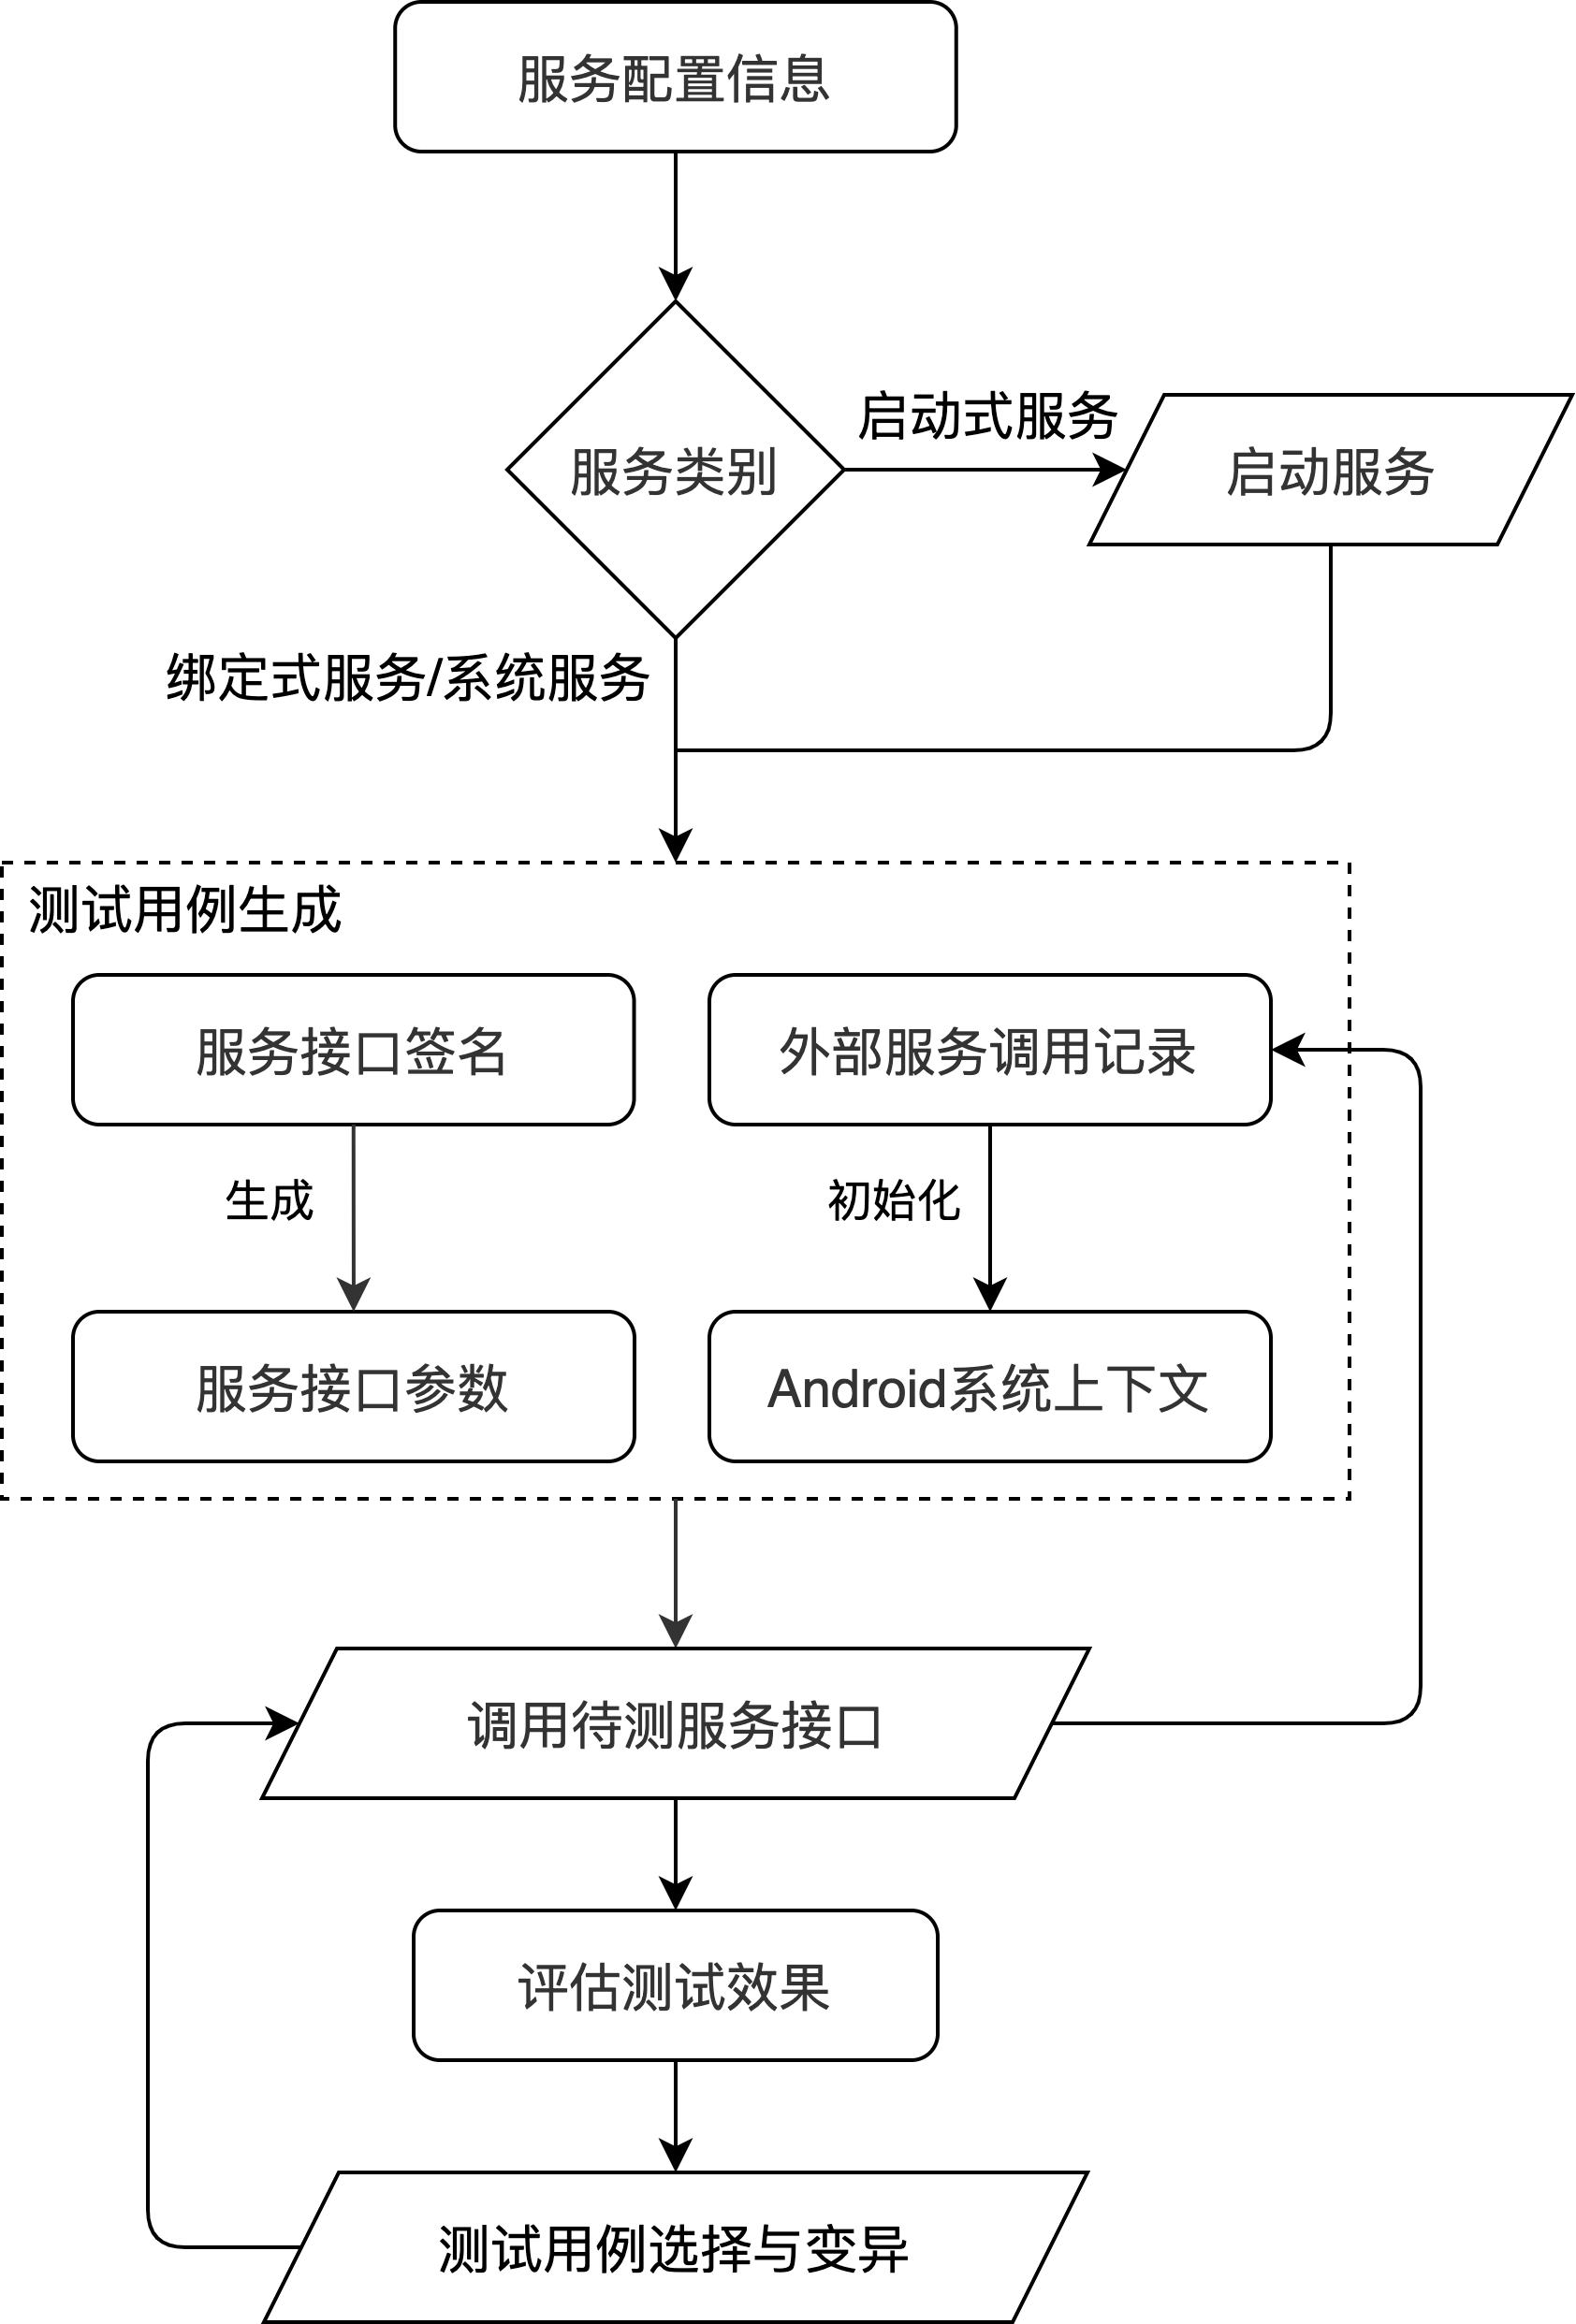
\includegraphics[width=.7\textwidth]{figure/4-fuzzer/workflow.png}
	\caption{模糊测试迭代过程}
	\label{workflow}
\end{figure}

CASFuzzer定义的服务测试用例包含待测服务标识符descriptor、接口编码code、服务接口参数parameters以及Android系统上下文MockDroidContext四个维度的参数,基于服务接口签名对这些参数进行生成与变异,通过基本块覆盖率来评估测试用例的效果,以指导模糊测试过程的迭代。

服务模糊测试的工作流程如图\ref{workflow} 所示:
\begin{itemize}
	\item 选择待测服务接口,根据服务类型及配置启动待测服务;
	\item 基于服务接口签名生成接口输入参数;
	\item 随着测试的迭代,收集外部服务调用记录,以初始化Android系统上下文;
	\item 装载Android系统上下文,调用待测待测服务接口;
	\item 根据测试效果,外部服务调用值与接口参数一起进行选择与变异。
\end{itemize}

\subsection{启动待测服务}

\textbf{系统服务} \quad 对于位于system\_server、mediaserver、cameraserver等守护进程中的系统服务来说,每个服务以线程的形式运行,只要同一进程中任意服务出错,进程中的WatchDog模块会监测到这一异常并退出整个进程。这些守护进程的启动参数记录在init.rc配置文件中,由Android系统中的init根进程所管理,一旦某个服务进程退出则会被init根进程自动重启。因此,在测试开始前只需等待对应系统服务自动运行即可,无需手动构造服务启动参数。

\textbf{应用服务} \quad 根据Android系统对服务生命周期管理方式的不同,可分为启动式服务与绑定式服务两类,判断的标准是服务是否实现了onStartCommand接口,启动式服务需要手动构造启动参数,绑定式服务则无需手动启动:
\begin{itemize}
	\item 对于启动式服务来说,关键是构造有效的启动Intent,我们沿用已有工作\cite{zhang2017systematically}\cite{yang2014intentfuzzer}中的Intent构造方法,对待测服务的onStartCommand函数进行轻量的静态分析,提取出Intent中component、action、category等属性的约束条件,使用约束求解器计算出对应的值,以此构造启动Intent。
	\item 对于绑定式服务来说,它的生命周期由Android框架来管理:当第一个客户端绑定服务时,该服务会被Android框架自动启动;当所有客户端均与服务取消绑定后,Android框架会自动销毁该服务。Android框架会检查绑定客户端的应用权限,为提高启动服务的成功率,需要将客户端应用置于system用户下。Android系统通过签名机制来保证敏感应用不会被篡改,所有system用户下的应用必须被厂商私钥签名,因此我们无法将应用添加到system用户下。为了绕过这一限制,我们拦截待测服务进程中IPCThreadState::getCallingUid函数调用,当服务绑定请求来自于客户端应用时,返回system用户的UID。
\end{itemize}

应用服务启动成功后,它的配置信息由ActivityManagerService维护在ServiceRecord对象中。通过ActivityManagerService服务的dump接口,即可获得所有应用服务的配置信息,从中提取出应用的PID、UID等字段,以便在后续的测试中追踪待测服务的运行时状态。

\subsection{模拟Android系统上下文}

模拟Android系统上下文MockDroidContext由一组对Binder IPC的劫持规则构成,包括Binder IPC匹配规则BinderIPCFilter以及接口的模拟返回值reply。BinderIPCFilter包含请求的外部服务标识descriptor、外部服务接口编码code以及请求参数匹配规则,匹配规则较为简单,直接对Parcel对象逐字节进行比较即可。

用户空间内的客户端进程一般通过IPCThreadState与Binder驱动进行交互。由于libbinder.so导出了IPCThreadState::transact函数符号,所有使用Binder通信机制的进程一定会链接libbinder动态连接库。因此通过hook目标进程中libbinder动态链接库的IPCThreadState::transact函数,即可拦截目标进程的所有Binder通信请求。

\begin{lstlisting}[caption={hook目标函数签名},label={lst:ipcthreadstate_transact},language=C++,basicstyle=\footnotesize]
status_t IPCThreadState::transact(int32_t handle, 
                                  uint32_t code, const Parcel& data,
                                  Parcel* reply, uint32_t flags);
\end{lstlisting}

该函数的签名如代码\ref{lst:ipcthreadstate_transact} 所示,在transact函数执行结束后,执行hook逻辑,根据作为函数参数的code以及data,以及可从data对象开头提取出的服务标识descriptor,我们即可对BinderIPCFilter规则逐个进行匹配,一旦满足条件,则将reply对象内容替换为mock返回值。

\begin{algorithm}[htbp]
	\caption{MockDroidContext迭代更新算法}
	\label{alg:state_update}
	\begin{algorithmic}[1]
		\REQUIRE $ctx$代表MockDroidContext的劫持规则集合,$max\_mut$最大变异次数,$s\_len$劫持规则数量限制
		\STATE $better$ $\gets$ 0
		\WHILE{$better$ < Min($max\_mut$, Len(ctx))}
		\STATE <$filter$, $reply$> $\gets$ RandomSelect($ctx$)
		\STATE $mut\_ctx$ $\gets$ $ctx$ $\cup$ $\{$<$filter$, Mutate($reply$)>$\}$
		\IF{ Fuzzing($mut\_ctx$).cov > Fuzzing($ctx$).cov }
		\STATE $ctx$ $\gets$ $mut\_ctx$
		\STATE $better$ $\gets$ $better$ + 1
		\ENDIF
		\ENDWHILE
		\STATE $record$ $\gets$ 更新外部服务接口访问记录
		\FOR{$r$ $\in$ $record$}
		\IF{<$r$.descriptor, $r$.code> $\in$ $ctx$} 
		\STATE $ctx$.Update($r$)
		\ELSE
		\STATE $ctx$.Append($r$)
		\ENDIF
		\ENDFOR
		\IF{Len($ctx$) > $s\_len$}
		\STATE $ctx$ $\gets$ LRU($ctx$,$s\_len$)
		\ENDIF
	\end{algorithmic}
\end{algorithm}

MockDroidContext的迭代更新算法如\ref{alg:state_update} 所示。测试工具一开始执行时,MockDroidContext为空,在测试迭代一段时间后,查询外部服务接口访问记录,以此为种子初始化劫持规则集合。测试迭代过程中,随机选择劫持规则,对其返回值进行变异,若测试反馈效果好,则更新MockDroidContext。当劫持规则集合的变异次数达到一定上限时,查询获得最新的外部服务接口访问记录,对劫持规则集合进行更新。过于复杂的劫持规则会导致过多Hook被加载到待测服务进程上,影响待测服务的执行效率,因此使用LRU策略淘汰长时间没有匹配成功的劫持规则。

\section{总体框架设计}

\begin{figure}
	\centering
	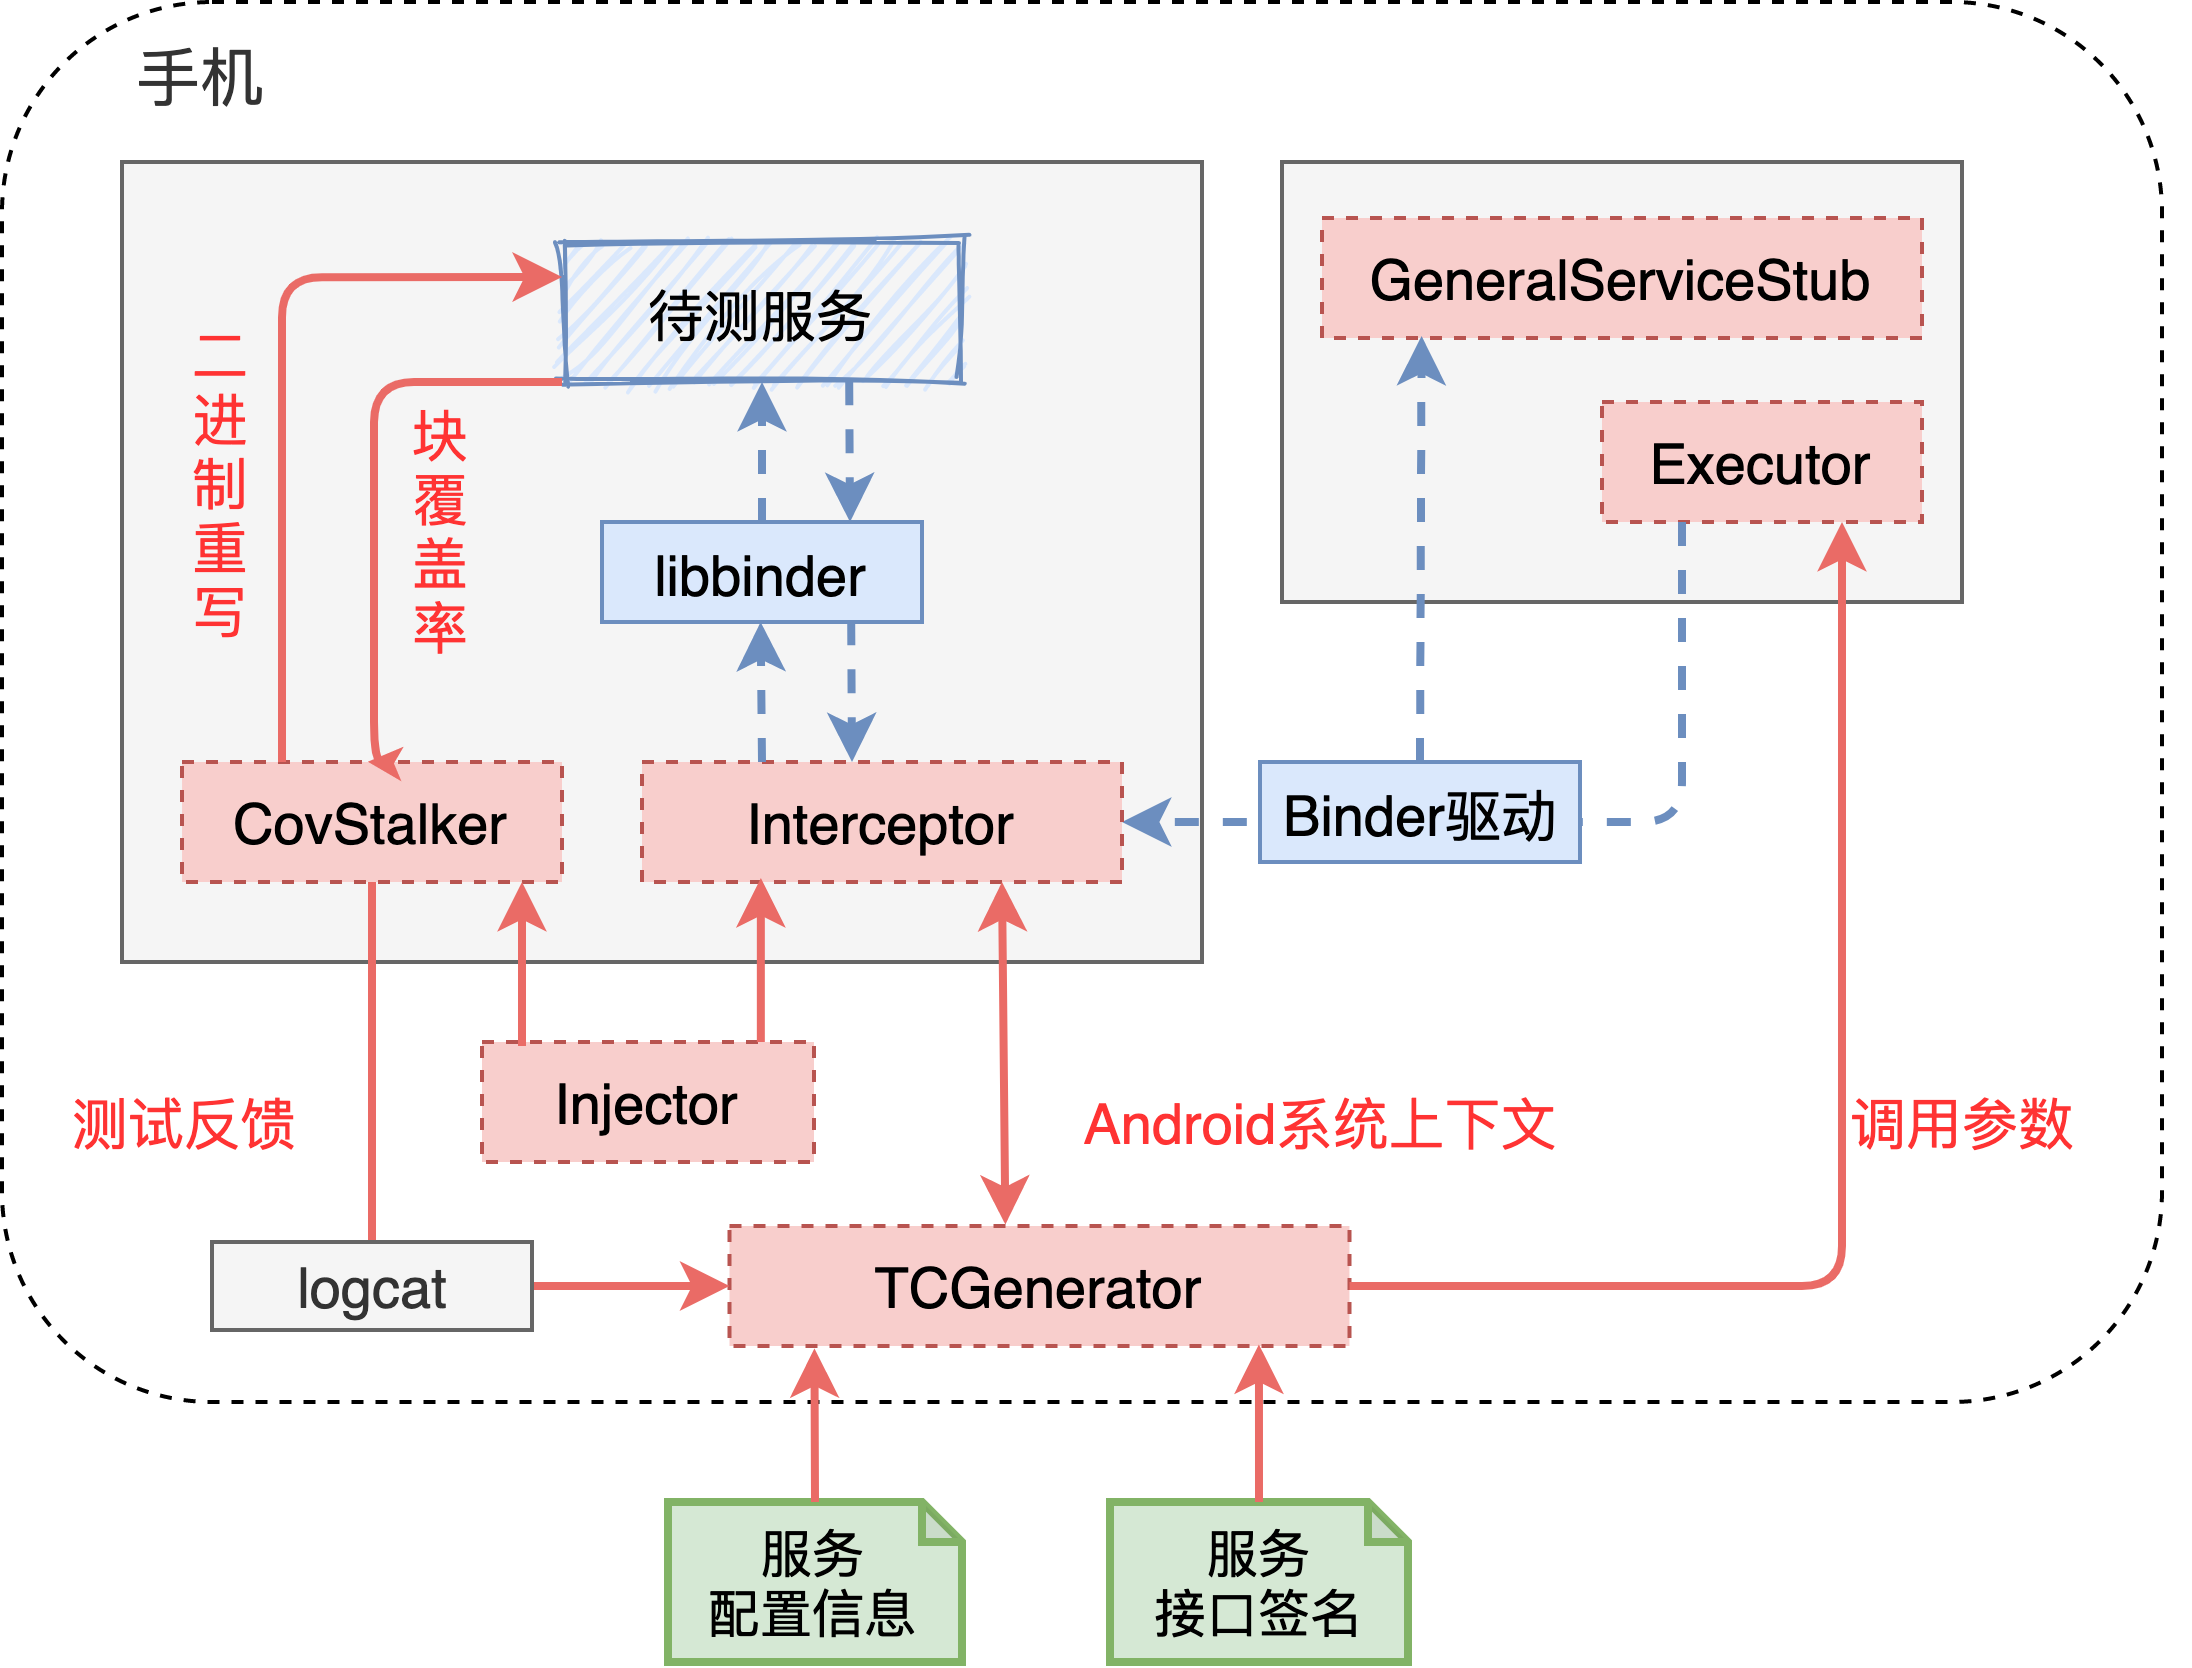
\includegraphics[width=.9\textwidth]{figure/4-fuzzer/arch.png}
	\caption{总体框架}
	\label{fuzzer-client}
\end{figure}

服务模糊测试工具CASFuzzer主要有以下几个核心模块,其各部分的实现情况如表\ref{tbl:loc} 所示:

\begin{table}[!htbp]
	\centering
	\begin{tabular}{cccc}
		\toprule
		模块名称 & 编程语言 & 编程框架 & LoC \\
		\midrule
		Injector & C++ & Frida & 620 \\
		CovStalker \& Interceptor & C++ & Frida & 3412 \\
		Ececutor \& GeneralServiceStub & Java & Android & 1528 \\
		TCGenerator & Java & \ & 5659\\
		\hline
		总计 & & &11219 \\
		\bottomrule
	\end{tabular}
	\caption{CASFuzzer模糊测试工具各模块实现情况}
	\label{tbl:loc}
\end{table}

其中Frida \cite{frida}是一款基于动态插桩技术实现的Hook框架,支持Android、iOS、Windows、Linux、MacOS等各种主流平台,兼容x86、ARM等多种指令集,提供Javascript、Python、C++等多种语言的交互接口。

\textbf{TCGenerator} \quad 是整个工具的核心模块,首先根据配置信息启动待测服务,读取服务接口签名以生成测试用例,确保mock的Android系统上下文已被Interceptor模块所装载后,让Executor模块调用待测服务,从CovStalker模块和logcat中获取测试结果反馈,改进测试用例并重复以上步骤。以单独Java进程的形式运行,将执行中间结果保存在SQLite本地数据库中。

\textbf{Injector} \quad 负责将CovStalker和Interceptor模块注入到待测服务进程之中,当待测服务重启后,模块会被重新注入。

\textbf{CovStalker} \quad 被注入到待测服务进程之中,通过动态二进制插桩(dynamic binary instrumentation)的方法修改目标进程的控制流,以记录基本块的访问情况,计算出基本块覆盖率,以Unix Domain Socket的形式提供给TCGenerator模块覆盖率查询接口。

\textbf{Interceptor} \quad 被注入到待测服务进程之中,在Binder IPC层面记录并劫持服务接口调用。TCGenerator模块会定期向Interceptor模块查询外部服务接口调用记录,以指导生成MockDroidContext。
Interceptor模块会记录下大量的外部服务接口调用记录,然而系统上下文不是一成不变的,随着测试的执行,对于同一服务接口的调用记录会覆盖旧有记录。由于Interceptor模块是以一个线程的模式运行在待测服务进程之中,当待测服务进程退出时,模块内保存的调用记录也会随之清空。

\textbf{Executor} \quad 以Android应用的形式存在,从TCGenerator模块获取服务参数,根据服务标识符descriptor从Service Manager或ActivityManagerService获取待测服务的IBinder对象,手动完成Parcel对象的序列化,调用IBinder对象的transact方法以完成接口调用。

\textbf{GeneralServiceStub} \quad 以Executor应用中的一个Service组件的形式存在,负责模拟IBinder类型对象,按照该对象的接口签名响应onTransact请求。


\section{测试用例生成策略}

我们将测试用例中涉及到的数据类型分为静态和动态两类,其中静态数据类型通过事先约定的规则即可生成,而动态数据类型需要结合程序运行时上下文才可确定。对于AIDL接口支持的六类数据类型中:基本数据类型、基本数据类型数组、Bundle类型、Parcelable类型、FileDescriptor类型属于静态数据类型;IBinder属于动态数据类型。虽然FileDescriptor类型代表的是进程中打开的文件描述符,只有在程序运行时才能生成,但决定文件特征的文件名、权限、内容等属性依然是可以按照静态的规则预先生成,因此我们还是将FileDescriptor类型归为静态数据类型。

\subsection{原始数据类型}

byte、int、float等原始数据类型的生成及变异策略如表\ref{tbl:primitive_type_generation} 所示。值得一提的是,int变量常常用于存储UID/PID等值,因此将待测服务或者Executor模块的UID/PID作为候选值之一。

\begin{table}[!htbp]
	\centering
	\begin{tabular}{ccc}
		\toprule
		AIDL数据类型 & 候选值 & 变异策略 \\
		\toprule
		boolean & true,false & 取反 \\
		\hline
		byte & 0, 1, -1, -128, -127 & 字节反转、加上随机值 \\
		\hline
		char & 0, 0xffff, ASCII & 字节反转、加上随机值 \\
		\hline
		\multirow{3}*{int} & 0, 1, -1, $2^{31} - 1$, $-2^{31}$ & 取负、加上随机值 \\
		\cline{2-3}
		& 待测服务 PID/UID & \multirow{2}*{无} \\
		& Executor模块 PID/UID & \\
		\hline
		long & 0, 1, -1, $2^{63} - 1$, $-2^{63}$ & 取负、加上随机值 \\
		\hline
		float & 0, 0x7fc00000, 0x1, 0x7f7fffff & 取负、加上随机值 \\
		\hline
		\multirow{2}*{double} & 0, 0x7ff8000000000000 & \multirow{2}*{取负、加上随机值} \\
		& 0x1, 0x7fefffffffffffff &  \\
		\bottomrule
	\end{tabular}
	\caption{基本数据类型的生成策略}
	\label{tbl:primitive_type_generation}
\end{table}

\subsection{String类型} 

String类型变量有三类取值:应用包名、应用权限permission、其他常量字符串。应用包名的候选值来自于待测ROM中所有的预装应用。对于permission的候选值,从对应Android系统版本的文档中可提取出system-permission,从预装应用AndroidManifest可提取出custom-permission。对于常量字符串的候选值,从DEX和ELF这两种编译产物中提取常量字符串:

\textbf{DEX中字符串} \quad 按照DEX的文件格式定义\cite{dex_format},string\_ids段以数组的格式存储了所有字符串在data数据段中的偏移量。根据偏移量从data读取到的数据中,第一个字节代表字符串长度,之后内容为字符串的值。

\textbf{ELF中字符串} \quad ELF中把常量字符串的索引保存在.strtab字符串表中,如果字符串表不存在,则遍历.rodata从中提取出所有合法的ASCII码字符串。

\subsection{Bundle类型} 

Bundle类型本质上是一个键值对形式的Map,key为String类型,value有多种类型可选:bool、int、long、double、String、上述类型的数组以及嵌套的Bundle对象。Bundle被用于Intent中用于携带额外的信息。有三个维度的变量需要考虑:内部Map的大小、key字符串的值、value的类型及具体值。

\subsection{Parcelable类型} 

Parcelable类型代表的是一个可通过Binder通信机制传输的复杂结构体。序列化数据由其内部成员变量的序列化数据依次拼接而成,前文所述的Parcel序列化API识别方法在遇到Parcelable类型时,会从该对象的writeToParcel方法中识别出其内部成员变量的类型及序列化顺序。

除此之外,若Parcelable对象可在Class Loader中用反射机制检索到对应的Java层对象,可以直接调用其构造函数生成,通过反射枚举出对象内部的成员变量,随机挑选变量进行变异,最后调用该对象的writeToParcel序列化方法即可。

\subsection{FileDescriptor类型}

代表的是客户端进程中一个合法的文件描述符,这个文件描述符不一定指向的是文件,也有可能指向Socket(如IConnectivityManager的establishVpn接口返回值为FileDescriptor,代表了服务端建立的VPN连接,由于这种情况并不常见,我们暂且不考虑文件描述符指向Socket的情况)。为使FileDescriptor指向的是一个合法的文件,我们使用Jimfs \cite{jimfs}在客户端进程内按照Android的目录命名规则构建一个虚拟的文件系统,文件有四个维度的变量需要考虑:

\textbf{文件名及所处目录结构} \quad 有两种目录格式:"/data/data/<package>/files/<name>"和"/mnt/sdcard/Android/data/<package>/files/<name>",对于应用服务来说,package为其所在的应用包名,对于系统服务来说,package可为系统上任何已安装应用的包名。

\textbf{UID/GID} \quad Android系统中使用UID/GID来管理应用程序的权限,在应用安装时由系统进行分配,之后不会再改变,应用私有目录的owner与应用的UID/GID一致。我们只考虑待测服务是否有权限访问文件这两种情况即可,对应于待测服务UID与AID\_NOBODY(9999)两个候选值。

\textbf{POSIX文件权限} \quad 由Owner权限、Group权限、Other权限三个整型数构成,整型数共有八种候选值。

\textbf{文件内容} \quad 简单起见,只考虑纯文本文件,沿用上述的String类型的生成方法即可,随机选用GBK、UTF-8、UTF-16三种编码方式。


\subsection{IBinder类型}

\begin{lstlisting}[caption={IBinder类型AIDL接口定义},label={lst:ibinder_type_example}]
interface IFoo {
  void foo(IFooCallback callback);
}
interface IFooCallback {
  bool action(int num);
}
\end{lstlisting}

如代码\ref{lst:ibinder_type_example} 所示,IBinder类型常常被用作在服务接口调用时传递回调函数或其他服务对象引用。对于待测服务接口IFoo.foo,需要构造实现了IFooCallback AIDL接口的IBinder服务对象。


已有的测试工作\cite{feng2016understanding}\cite{iannillo2017chizpurfle}\cite{liu2020fans}中,有两种IBinder类型构造方法:

\textbf{构造函数} \quad 将其作为一般的Object对象,通过Java反射调用构造函数生成。

\textbf{依赖重放} \quad 解析IBinder类型间的依赖,IBinder类型可作为其他接口的返回值,递归地调用其他接口,直到接口的参数只包含静态数据类型,将整条接口依赖链重放以生成目标IBinder类型。原理如图\ref{ibinder-dependency} 所示,待测服务为IFoo.method,需要IBinder型参数IBar,前序遍历依赖,发现IQux.method方法可返回IBar型对象,并且所有的参数都为静态类型,则构造接口参数调用IQux.method方法以生成IBar对象。

\begin{figure}
	\centering
	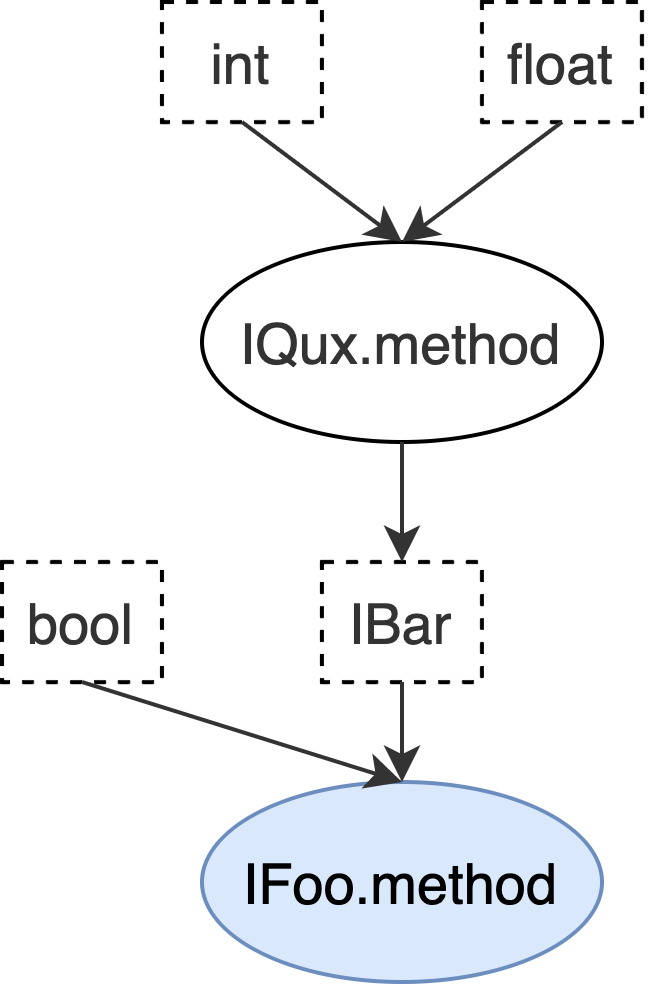
\includegraphics[width=.3\textwidth]{figure/4-fuzzer/ibinder-dependency.png}
	\caption{使用依赖重放的方法生成IBinder类型}
	\label{ibinder-dependency}
\end{figure}

这两种IBinder类型生成方法,都不能保证生成的成功率,而且由于生成的都是行为合法的IBinder类型,也不利于对待测服务的边界条件进行探索。

为了克服上述两点不足,受动态类型语言中“鸭子类型”的启发,我们在客户端进程中构造一个通用服务对象GeneralServiceStub,将所有作为参数的IBinder类型代理到GeneralServiceStub中,根据之前提取出的IBinder类型的内部服务接口签名,模拟其行为,还可生成行为异常(抛出异常、长时间阻塞等行为)的IBinder类型。



IBinder类型是指向其他服务(包括实名服务与匿名服务)的引用。构造IBinder类型的关键在于,对其所指向服务的行为进行模拟,它的行为可分为四种情况:

\textbf{服务正常处理请求} \quad 按照服务接口签名,返回类型合法的返回值。

\textbf{接口调用抛出异常} \quad Binder IPC中,服务端所抛出的RuntimeException会被传播到客户端。当异常的IBinder类型被作为参数传入待测服务接口时,待测服务接口对异常IBinder类型的使用可能会导致uncaught exception类型的crash。对应于代码\ref{lst:ibinder_type_example} 中的action函数调用抛出异常这种情况。

\textbf{接口调用阻塞} \quad 将调用阻塞的IBinder类型传入待测服务时,若对其接口的调用使得待测服务长时间持有某些资源锁,那么有可能会被系统中的watchdog机制判断超时,导致孵化进程zygote的重启,一般也称之为软重启。对应于\ref{lst:ibinder_type_example} 中的action函数阻塞这种情况。

\textbf{服务被销毁} \quad 当已被销毁的服务引用被传入待测服务时,对服务引用的调用会导致底层的Binder驱动出错并抛出异常,有可能导致uncaught exception类型的crash。对应代码于\ref{lst:ibinder_type_example} 中IFooCallback服务对象已被客户端Executor应用所销毁这种情况,对其的调用会导致Binder驱动报错。



\subsubsection{IBinder类型生成}

对于前三种服务行为,使用一个通用服务对象GeneralServiceStub来统一处理请求,所有测试用例中的模拟IBinder类型都是对GeneralServiceStub的引用。GeneralServiceStub对象的实现逻辑如代码\ref{lst:generalservicestub_impl} 所示。

\textbf{服务正常处理请求} \quad 由于我们只有服务的接口签名,并不知道服务接口的内部语义,只能按照接口签名的类型信息模拟合法的服务接口返回值,例如接口签名显示返回值为String类型,返回一个固定的字符串即可。

\begin{lstlisting}[caption={GeneralServiceStub实现逻辑伪代码},label={lst:generalservicestub_impl}]
class ServiceType {
  string                descriptor;
  Map<int, MethodType>  methods;
}
class MethodType {
  List<VarType>         parameters;
  VarType               reply;
}
Map<string, ServiceType>  typeModel;
class GeneralServiceStub {
  onTransact(code, request, reply) {
    // request的头部包含目标服务标识符descriptor
    descriptor = parse(request);
    serviceSig = typeModel.find(descriptor);
    methodSig = serviceSig.methods.find(code);
    // 检查调用参数类型是否匹配
    if(checkType(request, methodSig.parameters)) {
      // 按照前文所述的方法根据类型生成返回值
      reply = generateValue(methodSig.reply);
    }
  }
}
\end{lstlisting}

\textbf{接口调用阻塞} \quad onTransact函数在响应请求时阻塞住即可。

\textbf{接口调用抛出异常} \quad 当服务端抛出异常时,会将异常转换为错误码与对应的文本描述写入Parcel对象开头。值得一提的是,并不是所有的RuntimeException都会被传播,Android 8.1中只支持传播SecurityException、BadParcelableException、IllegalArgumentException、NullPointerException、IllegalStateException、NetworkOnMainThreadException、UnsupportedOperationException、ServiceSpecificException 9种异常,对应的错误码从-1到-9。onTransact函数只需往返回值reply对象中写入错误码即可。

\textbf{服务被销毁} \quad 从Binder驱动的角度来看,IBinder对象对应于指向binder\_ref结构的索引,若索引不合法,则Binder驱动会向上抛出异常。通过Interceptor模块修改Parcel对象中对应flat\_binder\_object对象的handle索引字段即可。

除了通过GeneralServiceStub来生成IBinder对象类型以外,还有一种策略是在运行时记录其他服务接口的返回值,若返回值是同一类型的IBinder对象,使用该返回值即可。但通过这种方法获得的IBinder对象,我们很难去修改它的行为,不容易探索到待测服务的边界值与异常情况。

\section{测试用例评估}

我们从待测服务或系统是否出现异常、基本块覆盖率是否提高两个指标来评价单个测试用例的执行效果,以此作为反馈来指导测试用例的迭代。

\subsection{异常日志监控}

通过Android系统的logcat工具监控系统日志中ERROR与FATAL级别的条目来判断待测服务是否抛出异常,同时为了监控Native服务进程的异常,还需监控 /data/tombstones目录下的核心转储coredump文件。

需要注意的是,由于服务之间普遍存在的依赖关系,单个服务的崩溃很有可能会导致大量服务的连锁崩溃(如system\_server中任一服务的崩溃会导致整个进程重启,致使系统中几乎所有的Java服务抛出异常)。从一系列异常日志中很难自动识别出根本原因,因此我们将所有异常日志先持久化到SQLite数据库中,后续由人工进行分析。

\subsection{基本块覆盖率}

主流的以覆盖率为指导的模糊测试工具中,AFL \cite{afl}与libFuzzer \cite{libfuzzer}在程序编译期间修改待测程序的中间代码表示,在基本块结尾插入覆盖率收集代码,kAFL \cite{schumilo2017kafl}在hypervisor层面利用Intel PT机制使用硬件记录程序执行的trace,以计算覆盖率信息。

以往针对Android应用的测试工具,大多只考虑了Java代码的覆盖率,通过字节码插桩\cite{acvtool}、类加载时插桩(load-time instrumentation)\cite{sun2017adrenalin}等技术实现。这些技术都属于侵入式的方法,需要对应用APK或者ART虚拟机进行修改。对于不能在模拟器环境下运行的闭源Android ROM来说,这些覆盖率收集方法并不适用。我们参考Chizpurfle中的方法,借助Frida框架提供的动态二进制插桩能力,修改待测程序控制流,以记录基本块的访问情况。

\begin{figure}
	\centering
	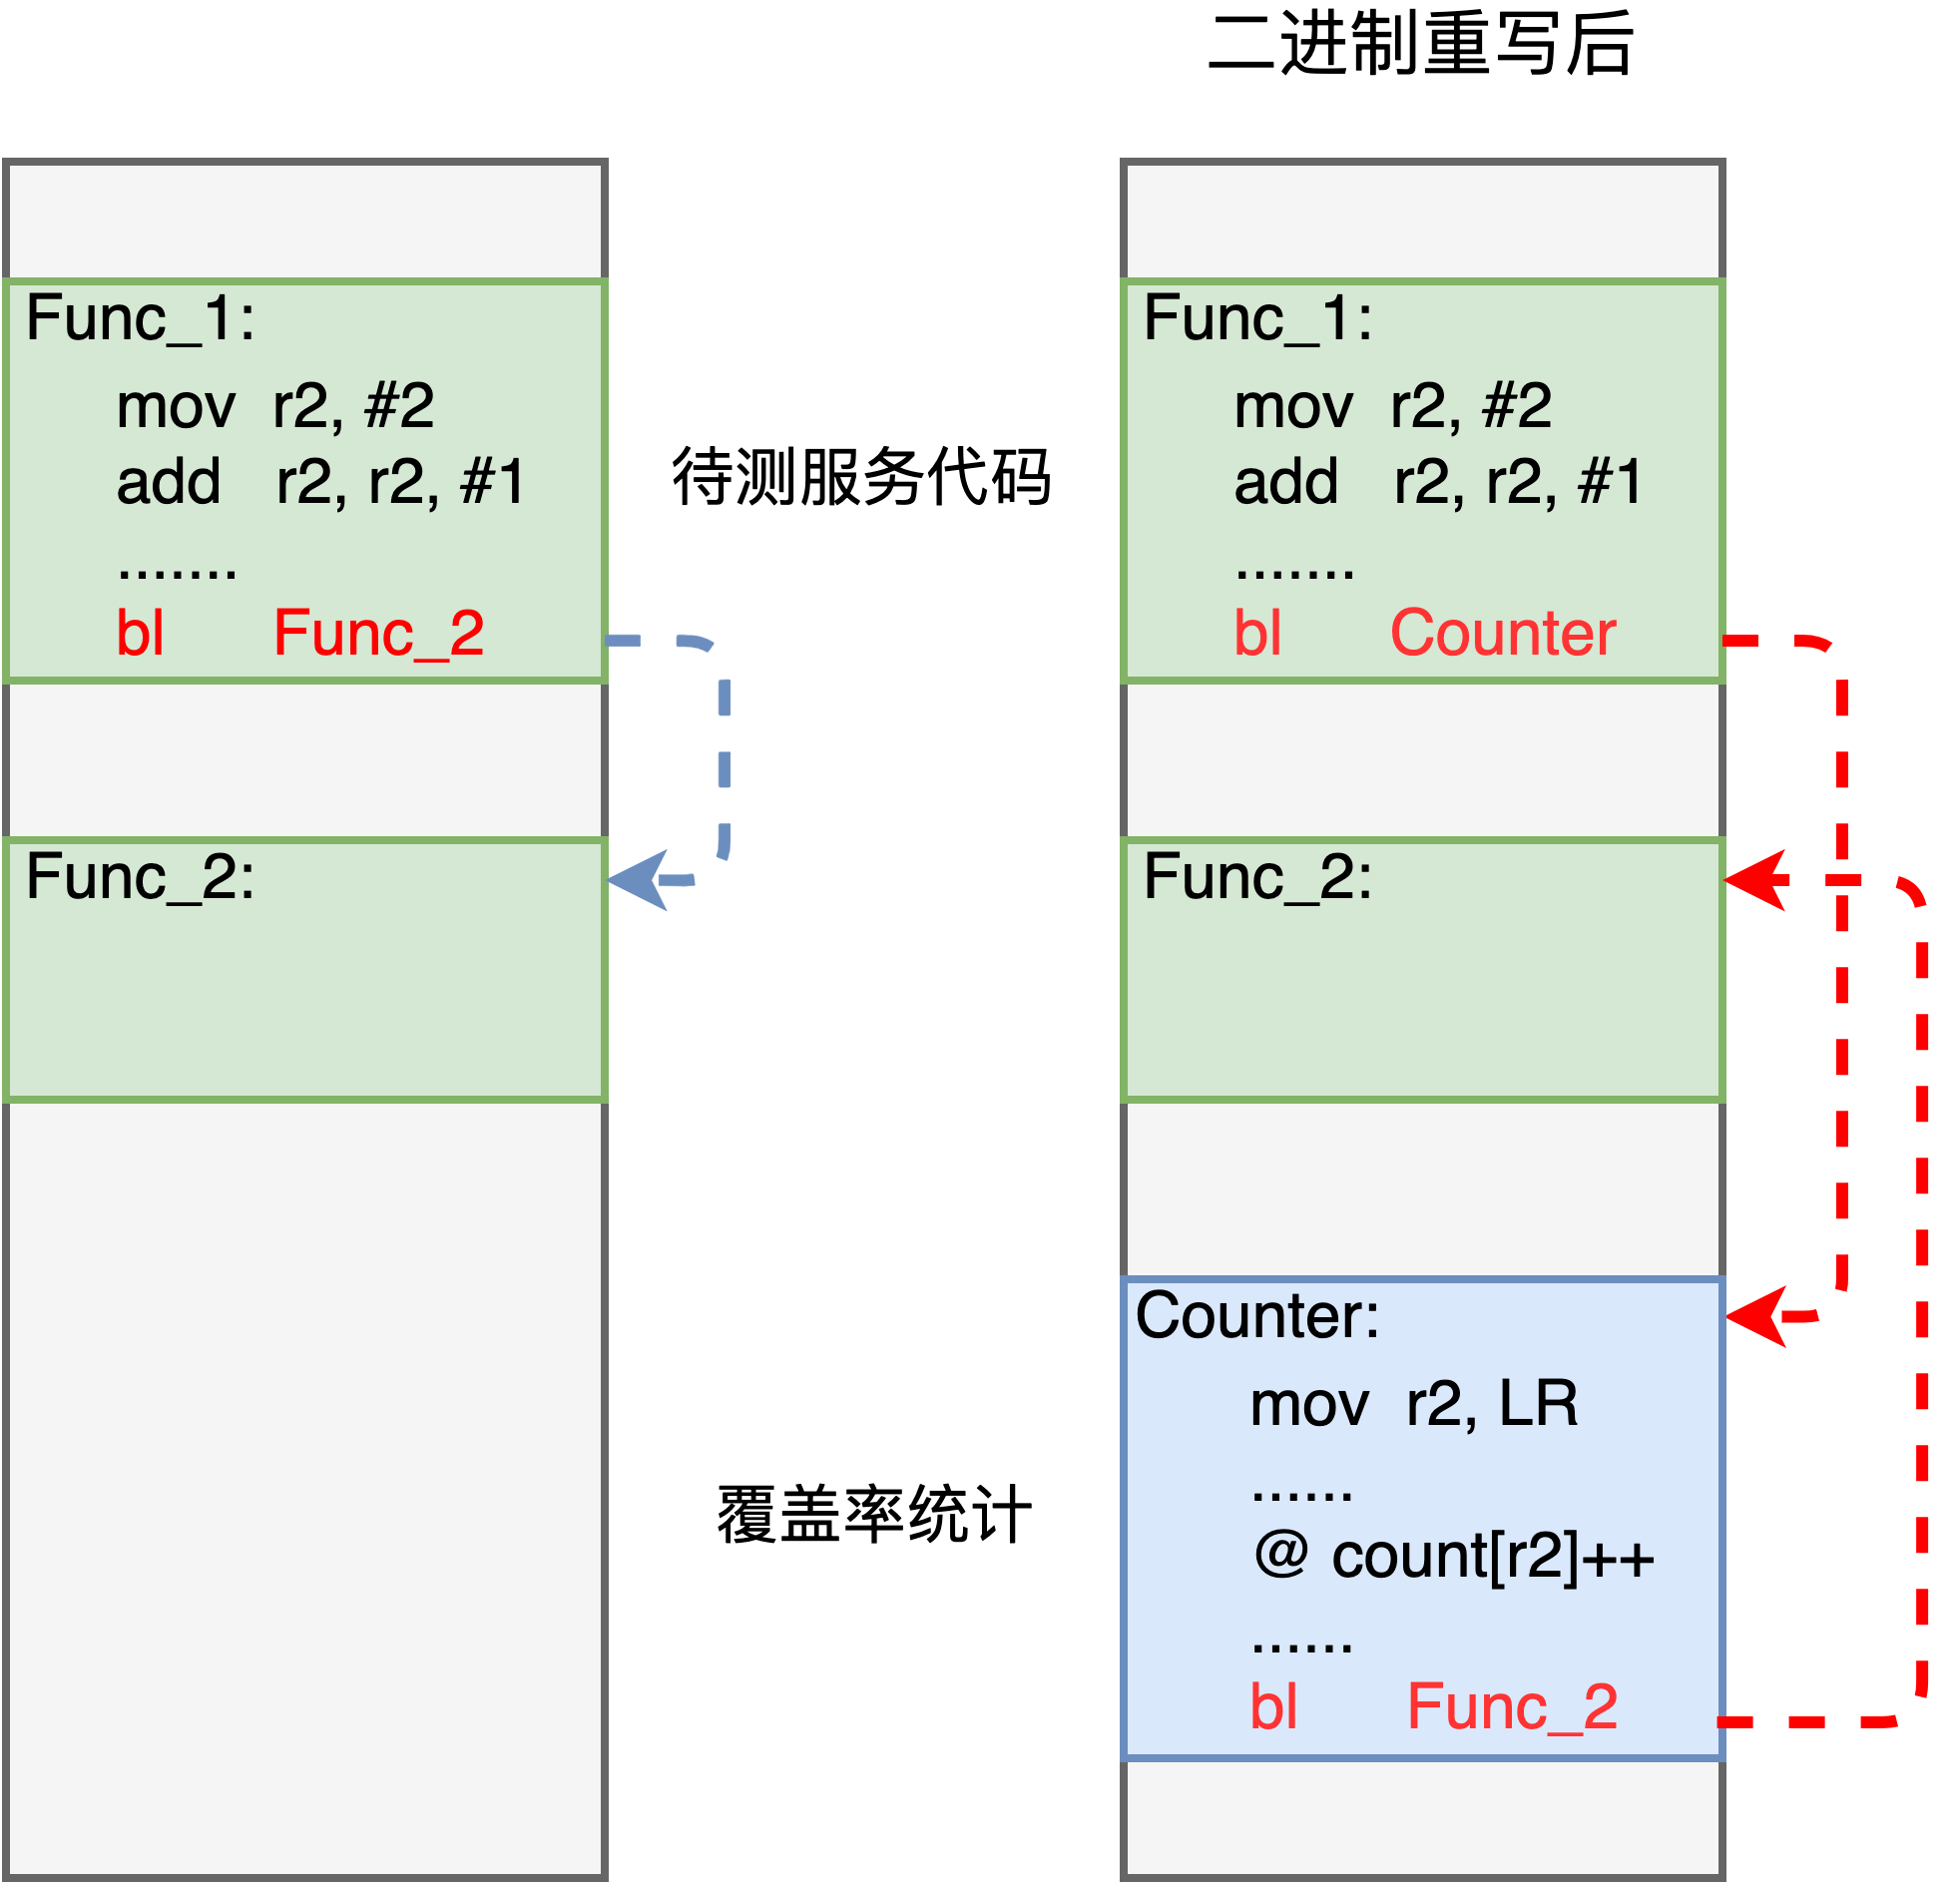
\includegraphics[width=.7\textwidth]{figure/4-fuzzer/bbcov-impl.png}
	\caption{基于动态二进制插桩的基本块覆盖率统计方法}
	\label{bbcov-impl}
\end{figure}

实现原理如图\ref{bbcov-impl} 所示,可分为如下六个步骤:
\begin{itemize}
	\item 挂起待测服务所处进程;
	\item 从当前程序寄存器所指代码位置开始,向后匹配分支跳转指令;
	\item 修改分支跳转指令的目标地址为Counter计数器代码段的首地址,并将跳转指令原本的目标地址保存到事先约定的内存地址中;
	\item 恢复待测服务进程执行;
	\item 当程序执行到二进制重写过后的基本块结尾跳转指令时,跳转到Counter计数器代码段;
	\item 从LR寄存器中读取先前基本块的末尾指令地址,以此为索引标记基本块被覆盖,在Counter计数器代码段的结尾,从事先约定的内存地址中读取指令在二进制重写前的跳转目标地址,跳回待测代码段,重复以上步骤;
\end{itemize}

基于上述方法实现了覆盖率收集模块CovStalker,以单个线程的形式运行在待测服务进程中,将每个线程的覆盖信息存储在对应的线程局部存储TLS(Thread-local Storage)中,以减少覆盖率计数器在线程切换时的运行开销。

需要注意的是,在Android系统中,单个进程中往往会运行若干个服务,每个服务以单独线程的形式运行,这些线程共享内存空间。因此很难单独计算出某个特定服务所对应的基本块总数,只能以整个进程地址空间所包含的基本块数量来近似计算基本块覆盖率。

\section{本章小结}

本章首先介绍了在测试用例中引入Android系统上下文的动机,然后介绍了如何使用Binder通信劫持的方式模拟Android系统上下文。基于此,我们设计了Android系统上下文感知的服务模糊测试工具CASFuzzer。接着介绍了CASFuzzer的基本框架,主要组件的功能以及模糊测试任务的执行流程。

然后介绍了CASFuzzer中的测试用例生成策略,包括静态数据类型和动态数据类型两类。静态数据类型的生成与其他模糊测试方法类似,主要通过预先定义的规则生成。动态数据类型包含IBinder类型,通过一个通用服务对象GeneralServiceStub将对IBinder类型对象的调用代理到本地的服务对象上,以模拟出接口调用异常、接口执行阻塞等异常行为。

最后介绍了如何收集测试结果反馈,包括异常日志的监控以及基于动态二进制插桩对基本块覆盖率的获取。

\chapter{实验评估}

\section{研究问题}

为了评估服务接口签名逆向工具RevExtractor对于不同类型服务的接口签名提取精度,我们以FANS和Chizpurfle中的服务接口签名提取方法为比较基准,在两个主流的定制Android系统以及两个版本的AOSP系统上进行实验评估;同时为了评估我们的服务模糊测试工具CASFuzzer的测试效果,我们在MIUI系统下进行实验评估。通过对实验结果的分析来回答如下问题:

\begin{itemize}
	\item 与FANS中基于C++源码静态分析的提取方法,以及Chizpurfle中基于运行时Java反射的提取方法相比,RevExtractor服务接口签名逆向工程的提取精度如何?
	\item CASFuzzer模拟的Android系统上下文,是否提高了模糊测试的效率?
	\item CASFuzzer生成的异常IBinder类型是否能发现特有的服务异常?
\end{itemize}

\section{实验配置}

\begin{table}[!htbp]
	\centering
	\begin{tabular}{cc}
		\toprule
		设备 & Android系统 \\
		\midrule
		小米手机5 & MIUI 10.8.11.22(基于Android 8.0)\\
		三星Galaxy C5 pro & Samsung Experience 9.0(基于Android 8.0)\\
		/ & AOSP 8.0.0\_r51(aosp\_arm64-user)\\
		/ & AOSP 9.0.0\_r61(aosp\_arm64-user)\\
		\bottomrule
	\end{tabular}
	\caption{测试设备配置}
	\label{tbl:device_list}
\end{table}

实验中使用到的测试设备以及Android系统如表\ref{tbl:device_list} 所示,包括MIUI与Samsung两款定制Android系统与两个版本的开源AOSP系统。小米与三星手机均使用该设备能兼容的最新版本的ROM\footnote{https://bigota.d.miui.com/8.11.22/miui\_MI5\_8.11.22\_f9ead04910\_8.0.zip}\footnote{https://samfw.com/firmware/SM-C5010/CHC/C5010ZCU2CRK1}进行刷机并ROOT。除此之外,我们在工作站上运行RevExtractor与FANS的静态分析组件,工作站配置如下:
\begin{itemize}
    \item 处理器:Intel(R) Xeon(R) CPU E3-1265L @ 2.40GHz
    \item 内存:16G
    \item 存储:500G SSD硬盘
    \item 操作系统:Ubuntu Server 18.04.5
\end{itemize}


\section{实验设计}

\subsection{服务接口签名提取}

从原理上来看,RevExtractor与FANS均使用静态分析的方法提取服务接口签名,而Chizpurfle在系统运行时通过Java反射提取服务接口签名。由于FANS的方法依赖于完整的Android系统源码,不能应用于闭源的定制Android系统之上,我们只能在开源的AOSP上比较RevExtractor与FANS针对Native服务的接口签名提取精度。为了评估RevExtractor对于Java服务接口签名的提取精度,我们与Chizpurfle在MIUI与Samsung Experience这两个定制Android系统上进行比较。

\subsection{模糊测试}

我们以小米手机5为测试设备,输入RevExtractor从MIUI ROM中提取出的服务接口签名,运行模糊测试工具CASFuzzer,进行实验评估。

为了理解Android系统上下文对服务运行的影响,我们将Interceptor模块装载到MIUI系统中的CameraService与AudioService进程中(这两种Native服务也往往会被移动设备厂商深度定制,并与Android系统硬件进行频繁地交互,具有一定的代表性),统计Interceptor模块拦截到的Binder IPC请求。为了模拟这两种服务的真实运行负载,在统计服务发出的Binder IPC请求的过程中,在前台运行相关应用(对于CameraService,运行相机应用;对于AudioService,运行音频播放器应用),并使用Monkey工具\cite{monkey}生成随机的GUI输入以模拟应用的使用。

为了评估模拟Android系统上下文对测试覆盖率的提升,我们以C++实现的CameraService与Java实现的SysoptService(MIUI新引入的服务,负责管理后台同步设置)为待测服务,分别在是否模拟Android系统上下文两种情况下,运行模糊测试工具15分钟,统计待测服务的基本块覆盖情况。

\section{结果分析}

\subsection{服务接口签名提取精度}

\begin{table}[!htbp]
	\centering
	\begin{tabular}{ccc|cc|cc|cc|c}
		\toprule{}
		工具 & Android系统 & \multicolumn{2}{c}{系统服务} & \multicolumn{2}{c}{服务接口} & \multicolumn{2}{c}{内部服务} & \multicolumn{2}{c}{接口准确性} \\
		& & $N_j$ & $N_n$ & $N_j$ & $N_n$ & $N_j$ & $N_n$ & $A_j$ & $A_n$\\
		\midrule
		RevExtractor & MIUI               & 134& 22 &3662&592 &488 &365&99.6\%&/     \\
		Chizpurfle   & MIUI               & 116& 40 &3099& /  &330 & / &基准   &/     \\
		RevExtractor & Samsung            & 174& 34 &5316&641 &616 &482&99.4\%&/     \\
		Chizpurfle   & Samsung            & 159& 52 &4875& /  &551 & / &基准   &/     \\
		RevExtractor & AOSP 8.0           & 111& 36 &2532&505 &157 &255& /    &84.2\%\\
		FANS         & AOSP 8.0           & /  & 36 & /  &505 & /  &260& /    &基准   \\
        RevExtractor & AOSP 9.0           & 124& 42 &2677&518 &160 &255& /    &86.5\%\\
        FANS         & AOSP 9.0           & /  & 42 & /  &518 & /  &266& /    &基准   \\
		\bottomrule
	\end{tabular}
	\caption{系统服务接口签名提取结果}
	\label{tbl:extractor_comp}
\end{table}

\if false
\begin{table}[!htbp]
	\centering
	\begin{tabular}{ccc|cc|cc}
		\toprule{}
		定制Android系统 & 工具 & \multicolumn{2}{c}{系统服务} & \multicolumn{2}{c}{服务接口} & 接口签名准确性 \\
		& & $N_j$ & $N_n$ & $N_j$ & $N_n$ & $A_j$ \\
		\midrule
		MIUI 10.8              & RevExtractor & 134& 22 &3662&592 &99.6\%     \\
		MIUI 10.8              & Chizpurfle   & 116& 40 &3099& /  &基准        \\
		Samsung Experience 9.0 & RevExtractor & 174& 37 &5316&641 &99.4\%     \\
		Samsung Experience 9.0 & Chizpurfle   & 159& 52 &4875& /  &基准        \\
		\bottomrule
	\end{tabular}
	\caption{服务类型信息提取结果}
	\label{tbl:extractor_comp}
\end{table}

\begin{table}[!htbp]
	\centering
	\begin{tabular}{ccc|cc|cc}
		\toprule{}
		AOSP系统版本 & 工具 & \multicolumn{2}{c}{系统服务} & \multicolumn{2}{c}{服务接口} & 接口签名准确性 \\
		& & $N_j$ & $N_n$ & $N_j$ & $N_n$ & $A_n$\\
		\midrule
		8.0.0\_r51 & RevExtractor & 111& 36 &2532&505 &84.2\%\\
		8.0.0\_r51 & FANS         & /  & 36 & /  &505 &基准   \\
		9.0.0\_r61 & RevExtractor & 124& 42 &2677&518 &86.5\%\\
		9.0.0\_r61 & FANS         & /  & 42 & /  &518 &基准   \\
		\bottomrule
	\end{tabular}
	\caption{服务类型信息提取结果}
	\label{tbl:extractor_comp}
\end{table}
\fi

在四种Android系统上的服务接口签名提取结果如表\ref{tbl:extractor_comp} 所示。其中内部服务表示不能直接通过Service Manager检索到的匿名服务对象,对应于各种IBinder类型所指向的服务对象。$N_j$与$N_n$分别表示系统服务数量、内部服务数量、服务接口数量这三个指标在Java与C++层面的数量。$A_j$与$A_n$表示在Java与C++层面上暴露服务以及内部服务所包含接口的准确性,判断标准为接口编号、输入参数及返回值类型是否匹配,判断数据类型是否匹配时:
\begin{itemize}
	\item 若为原始数据类型、Bundle类型以及FileDescriptor类型,则类型名称匹配即可;
	\item 若为Parcelable类型,则需递归地比较其内部成员的数据类型及序列化顺序是否匹配;
	\item 若为IBinder类型,则需递归地比较它对应的具体服务对象接口签名是否匹配;
\end{itemize}

从提取出的服务及接口数量指标来看:

\textbf{Java层面} \quad RevExtractor比Chizpurfle可以获取到更多的服务对象与接口。这是因为有的Java系统服务是由预装应用所初始化的,这些Java对象不会被预加载到Zygote的Class Loader中,因此Chizpurfle不能通过反射获取到对象。

\textbf{C++层面} \quad 与FANS相比,RevExtractor可以提取出所有服务对象,可以提取出94.6\%的服务接口。这是因为有些服务的实现不是由AIDL自动生成的(如SurfaceFlinger等),这些服务的通信序列化函数并不是以switch-case结构组织。


从提取的接口签名准确性指标来看:

\textbf{Java层面} \quad Chizpurfle通过调用Service Manager的接口以获取服务在Java层的对象,并通过反射获得对象内部方法的签名。显然这样获得的类型信息一定是准确的,因此我们以Chizpurfle为比较基准,评估RevExtractor从字节码中逆向提取Java服务类型信息的精度。对于Chizpurfle不能获得的Java服务,我们通过DexClassLoader将应用APK手动加载到Class Loader中,反射获取类型信息,作为比较的基准。结果显示在MIUI与Samsung两种定制Android系统上,RevExtractor提取的Java服务接口签名的准确性为99.6\%与99.4\%,具有很高的精度。

\textbf{C++层面} \quad FANS的类型提取方法借助于Clang/LLVM的插件,重新编译Android系统以生成服务相关代码的抽象语法树,指导之后的静态分析过程。FANS基于源码的方式,提取的类型信息准确度很高。我们以FANS提取的接口签名为比较基准,评估RevExtractor从汇编中逆向提取Native服务接口签名的精度。结果显示在AOSP 8.0与9.0两个版本上,RevExtractor提取的Native服务接口签名的准确性为84.2\%与86.5\%,这是因为在代码编译过程中,会丢失很多类型信息。例如:对于read(dst, sizeof(Type))这个Parcel序列化API调用,sizeof运算符在编译期被常量展开,从汇编中无法推断出Type对应的具体类型;虚函数调用可能会被编译器优化为直接跳转指令。

\begin{table}[!htbp]
	\centering
	\begin{tabular}{ccccc}
		\toprule{}
		Android系统 & 预装应用数及UID分布 & 暴露服务数 & 内部服务数 & 服务接口数 \\
		           & ($U_s$ / $U_p$ / $U_m$ / $U_o$) &&& \\
		\midrule
		MIUI            & 216(19 / 7 / 0 / 190)& 243 & 116 & 2316 \\
		Samsung         & 276(47 / 10 / 2 / 217)& 319 & 252 & 5515 \\
		AOSP 8.0        & 78(5 / 2 / 2 / 69)& 97  & 32  & 1615 \\
		AOSP 9.0        & 79(5 / 2 / 2 / 70)& 99  & 32  & 1626 \\
		\bottomrule
	\end{tabular}
	\caption{预装应用服务接口提取结果}
	\label{tbl:extractor_preinstall_apps}
\end{table}

RevExtractor不仅考虑了系统服务,还对ROM中预装应用服务的接口签名进行了提取,结果如表\ref{tbl:extractor_preinstall_apps} 所示,其中$U_s$、$U_p$、$U_m$与$U_o$分别表示应用属于android.uid.system、android.uid.phone、android.media与其他用户。可以看出定制Android ROM中引入了大量的预装应用以及服务,这些服务组件有很多都属于暴露服务,容易被攻击者所利用。不仅如此,这些预装应用有不少位于system等系统用户下,具有很多敏感的应用权限,而以往研究很少关注于这类应用,我们将预装应用中的服务组件也纳入到测试对象中。

\begin{figure}
	\centering
	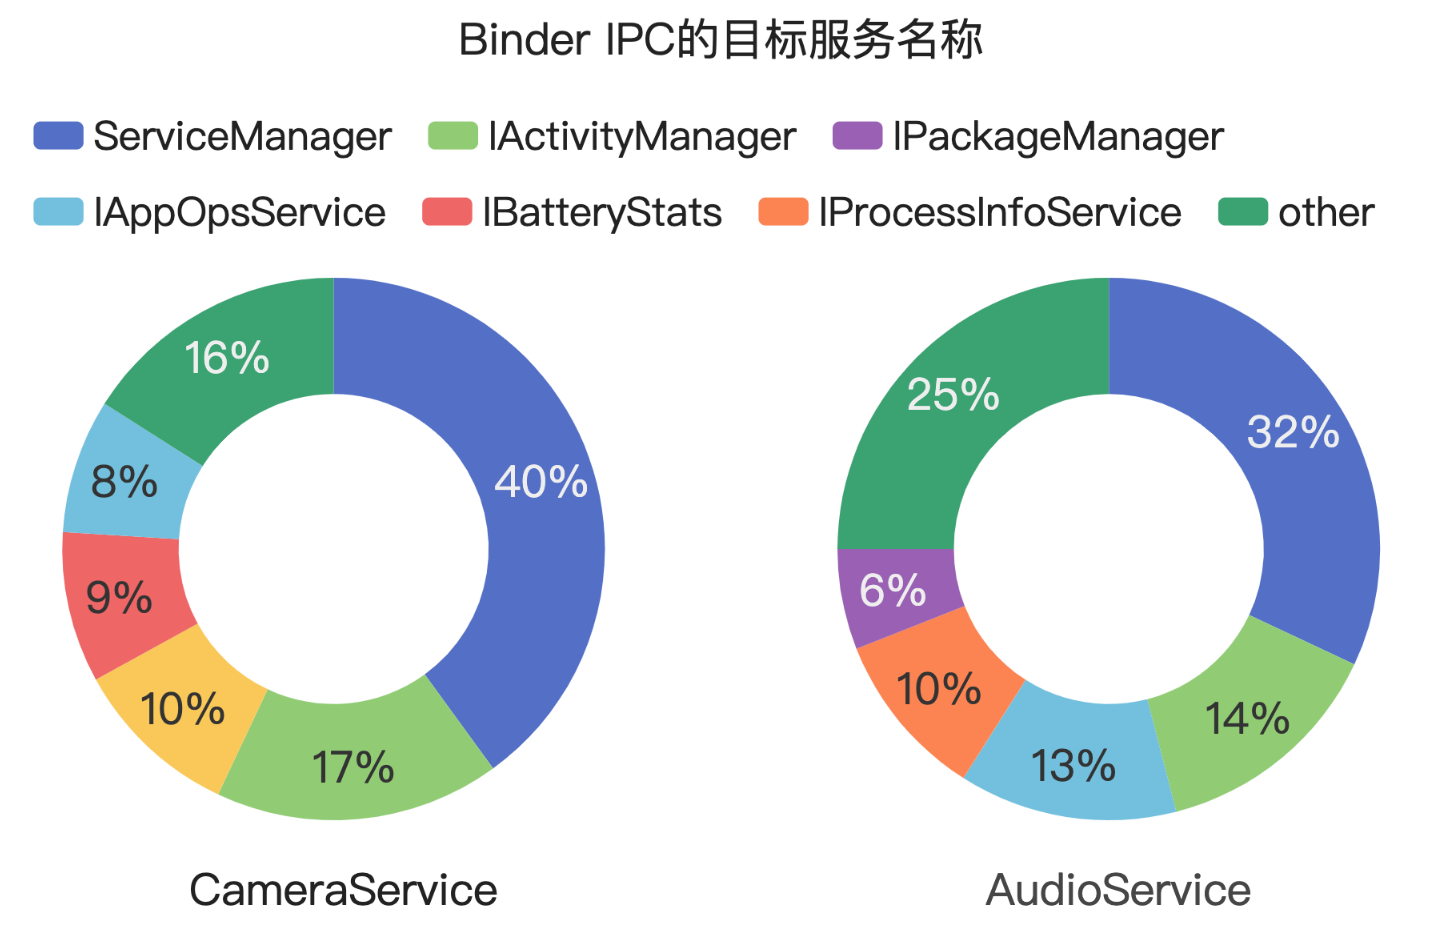
\includegraphics[width=\textwidth]{figure/5-experiment/binder-ipc-record.png}
	\caption{不同服务拦截到的Binder IPC分布}
	\label{binder_ipc_stats}
\end{figure}

\subsection{服务模糊测试效果}

\subsubsection{模拟Android系统上下文对测试效果的提升}

\begin{figure}
	\centering
	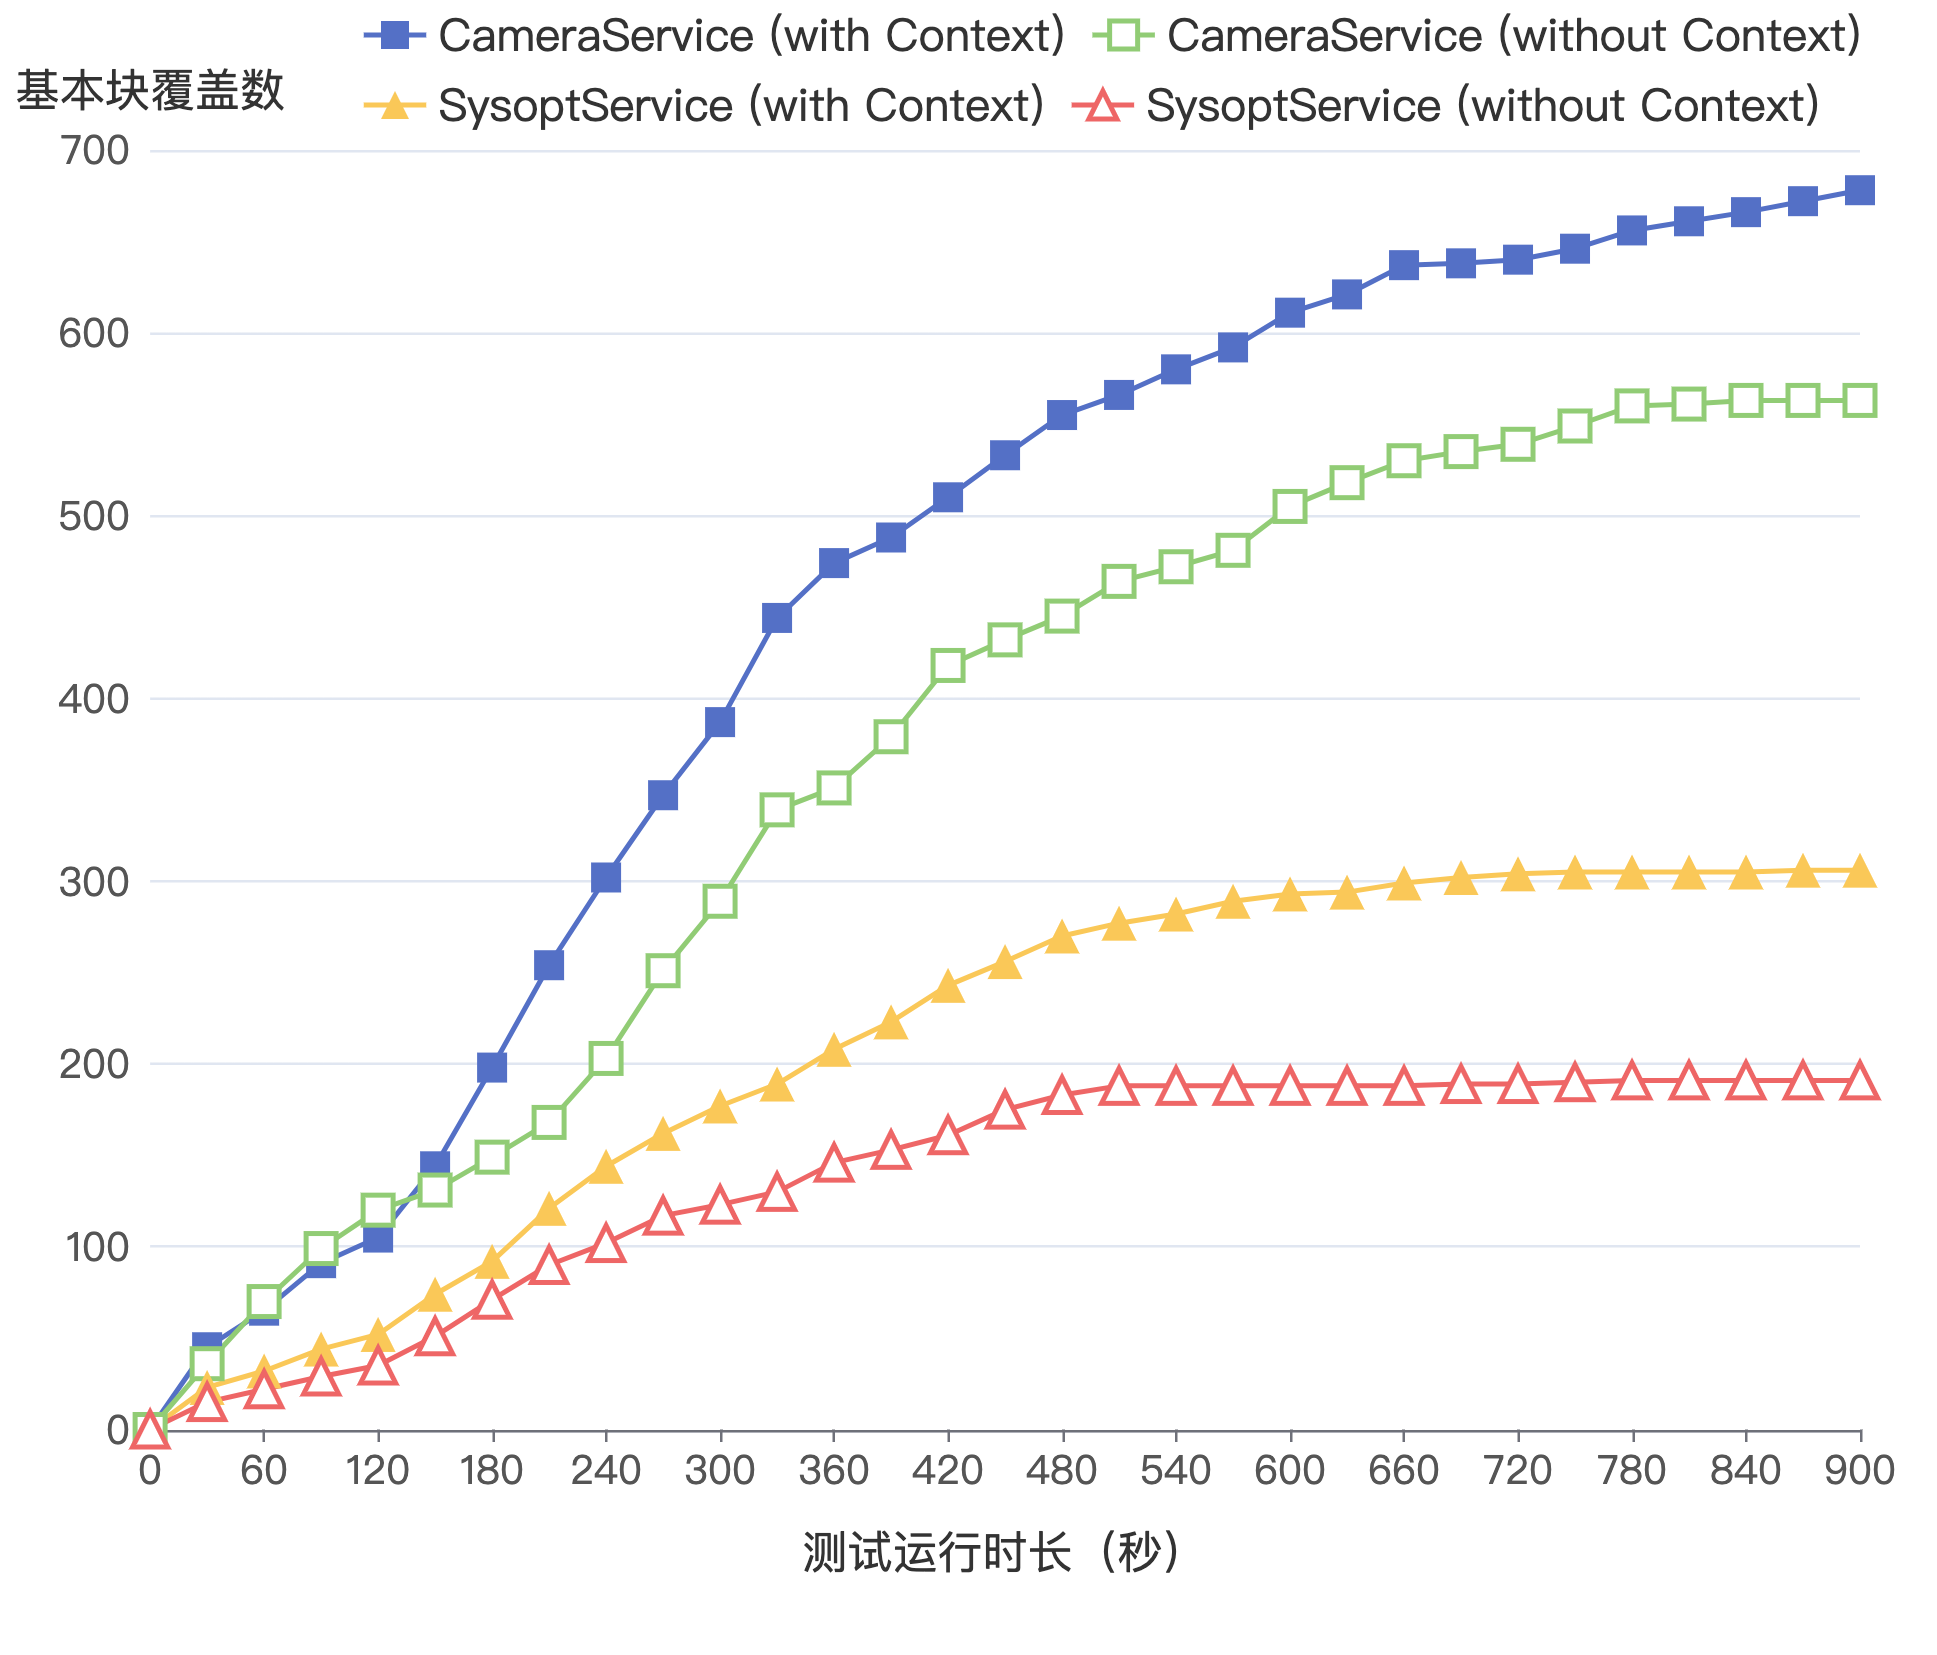
\includegraphics[width=\textwidth]{figure/5-experiment/cov-inc-with-context.png}
	\caption{模拟Android系统上下文对测试覆盖率的提升}
	\label{coverage_with_context}
\end{figure}

对于MIUI系统中的CameraService与AudioService服务,提取Interceptor模块拦截到的Binder IPC请求中包含的目标服务名称,其分布情况如图\ref{binder_ipc_stats} 所示。

拦截到的Binder IPC请求中,对Service Mangnager的访问请求占比最大,这是因为Service Manager是所有服务的注册中心,需要先从中获取到其他服务的IBinder引用,才可使用这些外部服务接口,对于这类Binder IPC请求我们不进行拦截,以便待测服务能继续执行。

除此之外,其他服务请求的对象主要包括ActivityManager、PackageManager以及AppOpsService等与应用权限管理有关的服务,PowerManager等与能耗管理有关的服务,ProcessInfoService等系统状态有关的监控服务。对于权限管理服务请求的劫持,可以在不同应用权限配置情况下,测试待测服务的行为是否异常。对于PowerManager服务的请求主要集中在acquireWakeLock、acquireWakeLockWithUid这几个接口,如果劫持这些接口请求并模拟调用异常,则待测服务往往会直接退出。


对于以C++实现的CameraService与Java实现的SysoptService,在是否模拟Android系统上下文两种情况下,15分钟的模糊测试过程中基本块覆盖率情况如图\ref{coverage_with_context} 所示。实验结果显示,对于Java与Native服务,模拟的Android系统上下文,可以使得模糊测试过程更快地探索到待测服务新的基本块,还可以提高最终的服务测试深度。

\subsubsection{异常IBinder类型触发的服务异常}

\begin{table}[!htbp]
	\centering
	\begin{tabular}{cccc}
		\toprule
		类别 & 异常类型 & 数量 & 异常IBinder类型触发\\
		\hline
		\multirow{6}{*}{Java} & java.lang.NullPointerException & 28 & 2 \\
		& java.lang.IllegalStateException & 19 & 0 \\
		& android.os.DeadObjectException & 15 & 14 \\
		& java.lang.SecurityException & 7 & 0 \\
		& java.io.InterruptedIOException & 6 & 6 \\
		& android.os.TransactionTooLargeException & 3 & 0 \\
		\hline
		Native & SIGSEGV & 16 & 1 \\
		\midrule
		合计    &         & 94 & 23 \\
		\bottomrule
	\end{tabular}
	\caption{测试中发现的异常}
	\label{tbl:fuzzer_exception_list}
\end{table}

截止到目前的测试,我们在小米手机5的MIUI 10.8中发现的异常如表\ref{tbl:fuzzer_exception_list} 所示,总计触发了78次Java异常,16次原生代码奔溃。为了确定这些服务异常是否由异常IBinder类型所触发,相应的测试用例需要满足两个条件:服务接口参数中包含异常IBinder类型;将异常IBinder类型替换为正常值,服务异常不能被重现。结果显示,DeadObjectException与InterruptedIOException主要都是由异常IBinder类型触发的,而其他服务测试工具并没有发现这类特殊的服务异常。

需要注意的是,由于待测服务内部状态的不同,同一个测试用例并不一定能100\%触发服务异常,由于缺乏待测服务源码,并不能确定某个服务异常一定是由某种异常IBinder类型所触发。

在测试过程中发现,对于Native服务的模糊测试也可能会触发Java层面的Exception,反之亦然,这表明Java与Native服务之间存在复杂的依赖关系,这也导致我们在没有源码的情况下很难定位异常的根本原因。值得一提的是,有的原生代码崩溃会导致整个系统反复重启,必须人工重新刷机来修复,这不利于自动化测试的进行,并且会丢失CASFuzzer模块在设备本地使用SQLite保存下的所有中间结果,后续考虑切换到其他外部数据库来保存测试中间结果。


\section{本章小结}

首先为了评估服务接口签名逆向工具RevExtractor的有效性, 我们在MIUI、Samsung Experience、AOSP三种Android系统上,与FANS、Chizpurfle中的接口签名提取方法进行比较。实验结果显示,对于Java服务,RevExtractror有很高的准确度,对于Native服务,RevExtractror从高度精简的ARM汇编中依然可以提取出较为准确的类型信息。

接着我们使用服务模糊测试工具CASFuzzer对MIUI中的服务进行实验评估。实验结果显示,CASFuzzer对Android系统上下文的模拟使得测试过程更加深入有效,测试用例中模拟的异常IBinder类型可以触发特定的服务缺陷。

到目前为止,我们使用服务模糊测试工具CASFuzzer在MIUI 10.8中发现了94个服务异常。

\chapter{总结与展望}
\section{工作总结}

本文在Android服务测试相关研究工作的基础上,针对定制Android系统中的预装应用服务、Java系统服务与Native系统服务,提出包括服务接口签名提取、测试用例生成、测试结果反馈、测试用例迭代的整套自动化服务模糊测试方法。

实现了服务接口签名逆向提取工具RevExtractor,以逆向工程的方式,从服务的编译产物中推测出接口签名,具体来说包含三个步骤:从Android ROM中提取服务相关编译产物;结合Android系统运行时状态,筛选出待测服务的通信序列化函数;从通信序列化函数的字节码与ARM汇编中,识别出序列化过程结构特征,以此推测出服务接口签名。

基于生成式策略,实现了服务模糊测试工具CASFuzzer:通过Binder通信劫持技术,模拟影响服务执行的Android系统上下文,提高测试深度;通过模拟Android系统中特有的IBinder类型的异常行为,更好地探索待测服务的边界情况;基于动态二进制插桩收集被测服务的基本块覆盖率,使得模糊测试过程迭代更为高效。

经实验分析证实,在不同定制Android ROM中,RevExtractor工具可以逆向提取出较为精确的服务接口签名信息,并使用CASFuzzer模糊测试工具发现了MIUI 10.8中的90多处服务异常。

\section{研究展望}

我们下一步的研究内容可能从以下两方面着手:

\textbf{提取服务接口间的依赖} \quad Android系统中的服务往往都是有状态的,同一个服务不同接口调用间有隐含的依赖关系,甚至服务之间也会存在依赖关系,若接口调用顺序出错,服务会忽略该请求。例如ICameraService服务中调用removeListener接口前需要先调用addListener接口、IMediaBrowserService服务中调用disconnect接口前要先调用connect接口等。我们可以在Android系统运行时,收集服务接口调用记录,从这些历史记录中推测接口之间的依赖关系。

\textbf{高效地统计覆盖率} \quad 通过动态二进制插桩的方式会大大提高目标程序的运行开销(例如Valgrind内存分析框架在SPEC CPU 2006数据集上,运行速度平均慢4.3倍\cite{nethercote2007valgrind}),动态二进制插桩下的Android服务程序,运行开销至多可达10倍以上。通过CPU提供的硬件级别的程序执行追踪机制(如Intel的Branch Trace Store、ARM的CoreSight STM),以硬件辅助的方式高效地收集待测程序的覆盖率。



%%%%%%%%%%%%%%%%%%%%%%%%%%%%%%%%%%%%%%%%%%%%%%%%%%%%%%%%%%%%%%%%%%%%%%%%%%%%%%%
% 致谢,应放在《结论》之后


\begin{acknowledgement}

三年硕士生涯即将结束,在学位论文即将完成之际,我要向所有在此期间支持、帮助过我的人表达诚挚的感谢。

首先,感谢我的指导老师曹春教授。当初保研时,有幸能得到导师的认可,让我能够跨专业进入计算机系攻读研究生。进入实验室以来,曹老师不仅提供了大量项目实践的机会,也引领我走进了软件工程研究领域的大门,他在为人处事上的淳淳教诲也让我收益匪浅。文本从选题、实验设计、论文撰写都离不开曹老师的指导,使我的毕业论文能够顺利完成。

感谢南京大学计算机系的各位老师,是你们精彩的课程吸引我进入计算机领域,也帮助我掌握了扎实的专业技能。感谢软件所各位老师和同学对我的关心和帮助,让我的研究生生活更加充实。

感谢葛红军、邓靖师兄对我Android自动化测试研究领域的引导,感谢陈洁、李青坪师兄对我云计算研究领域的引导。感谢实验室的师兄师弟们以及舍友们,在你们的陪伴下,度过了三年的难忘时光。

感谢我的家人们,在外求学期间,你们的关心和挂念,帮助我跨越求学路上的坎坷。

最后,感谢南京大学,提供了开放的学习氛围与优越的生活环境,伴我度过了愉快的七年求学时光。

此致,感谢!

\end{acknowledgement}


%%%%%%%%%%%%%%%%%%%%%%%%%%%%%%%%%%%%%%%%%%%%%%%%%%%%%%%%%%%%%%%%%%%%%%%%%%%%%%%




% 参考文献。应放在\backmatter之前。
% 推荐使用BibTeX,若不使用BibTeX时注释掉下面一句。
%\nocite{*}
\bibliography{sample}


% 附录,必须放在参考文献后,backmatter前

%%%%%%%%%%%%%%%%%%%%%%%%%%%%%%%%%%%%%%%%%%%%%%%%%%%%%%%%%%%%%%%%%%%%%%%%%%%%%%%
% 书籍附件
\backmatter
%%%%%%%%%%%%%%%%%%%%%%%%%%%%%%%%%%%%%%%%%%%%%%%%%%%%%%%%%%%%%%%%%%%%%%%%%%%%%%%
% 作者简历与科研成果页,应放在backmatter之后

\begin{resume}
% 论文作者身份简介,一句话即可。
\begin{authorinfo}
\noindent 廖祥森,男,汉族,1996年8月出生,江西赣州人。
\end{authorinfo}
% 论文作者教育经历列表,按日期从近到远排列,不包括将要申请的学位。
\begin{education}
\item[2018年9月 --- 2021年6月] 南京大学计算机科学与技术系 \hfill 工学硕士
\item[2014年9月 --- 2018年6月] 南京大学地理与海洋科学学院 \hfill 理学学士
\end{education}
% 论文作者在攻读学位期间所发表的文章的列表,按发表日期从近到远排列。
\begin{publications}
\item 发明专利:一种基于系统调用代理的安卓虚拟化方法及系统(专利号:202110557154.0)
\item 发明专利:一种基于逆向工程的安卓闭源服务类型信息提取方法(专利号:202110557657.8)
\item 软件著作权:软件SDK自动化测试云平台V1.0(登记号:2021SR0675157)
\end{publications}
% 论文作者在攻读学位期间参与的科研课题的列表,按照日期从近到远排列。
\begin{projects}
\item 国家重点研发计划:软件定义的人机物融合云计算支撑技术与平台(2018YFB1004805),2018年5月—2021年4月,负责云计算支撑平台的设计与实现。
\end{projects}
\end{resume}

%%%%%%%%%%%%%%%%%%%%%%%%%%%%%%%%%%%%%%%%%%%%%%%%%%%%%%%%%%%%%%%%%%%%%%%%%%%%%%%
% 生成《学位论文出版授权书》页面,应放在最后一页
\makelicense

%%%%%%%%%%%%%%%%%%%%%%%%%%%%%%%%%%%%%%%%%%%%%%%%%%%%%%%%%%%%%%%%%%%%%%%%%%%%%%%
\end{document}
